\documentclass{thesis}

\usepackage{biblatex}

\newcommand{\wydzial}{Wydzia\l{} Informatyki}
\newcommand{\katedra}{Katedra System\'ow Inteligentnych i Data Science}
\newcommand{\specjalizacja}{Data Science}
\newcommand{\imienazwisko}{Micha\l{} Chojna}
\newcommand{\nralbumu}{Nr albumu: s29758}
\newcommand{\tytulpracy}{Analiza efektywno\'sci r\'o\.znych architektur wieloagentowych w analizie dokument\'ow ubezpieczeniowych}
\newcommand{\rodzajpracy}{Praca magisterska}
\newcommand{\promotor}{dr hab.\ Andrzej Wodecki, prof.\ PJATK}
\newcommand{\miejscedata}{Warszawa, czerwiec 2026}

\renewcommand{\maketitle}{%
  \begin{alwayssingle}
    \thispagestyle{empty}

    \begin{center}
      \vspace*{-1cm}
      
\includegraphics[width=0.95\textwidth]{PJATK_PL_poziom_1}
    \end{center}

    \vspace{2cm}

    \begin{center}
      {\fontsize{14}{17}\bfseries \wydzial} \\[1.2cm]
      {\large\bfseries \katedra} \\[0.4cm]
      {\large \specjalizacja}
    \end{center}

    \vspace{1.8cm}

    \begin{center}
      {\large\bfseries \imienazwisko} \\[0.2cm]
      {\large \nralbumu}
    \end{center}

    \vspace{1.8cm}

    \begin{center}
      {\LARGE\bfseries \tytulpracy}
    \end{center}

    \vspace{2cm}

    \hfill
    \begin{minipage}{0.50\textwidth}
      \begin{flushleft}
        \rodzajpracy \\ [0.4cm]
        \promotor
      \end{flushleft}
    \end{minipage}

    \vfill

    \begin{center}
      \miejscedata
    \end{center}

  \end{alwayssingle}
}

\addbibresource{references.bib}

\begin{document}

\setcounter{secnumdepth}{3}
\setcounter{tocdepth}{3}

\maketitle

\begin{romanpages}
  \begin{abstract}
  W pracy zbadano wpływ topologii systemów agentowych na jakość odpowiedzi
  na pytania wymagające analizy dokumentów ubezpieczeniowych -- Ogólnych Warunków
  Ubezpieczenia (OWU) oraz dokumentów zawierających informacje o~produkcie
  ubezpieczeniowym (IPID).  Środowisko testowe wybrano ze względu na jego złożoność: specjalistyczny
  język prawniczo-ubezpieczeniowy łączy się z~wielopoziomową strukturą warunków
  i~wyłączeń rozproszonych w~wielu paragrafach. Wymagało to od badanych
  architektur skutecznego wykorzystania mechanizmów wyszukiwania i~wnioskowania.

  Porównano sześć architektur opartych na dużych modelach językowych
  (\textit{ang.}~\textit{Large Language Models}, LLM): deterministyczną,
  planer--wykonawca, router--specjalista, tablicową, hierarchiczną oraz ReAct.
  Bazę wiedzy systemu stanowiły 22 polskie dokumenty ubezpieczeniowe pochodzące
  od trzech głównych towarzystw ubezpieczeniowych. Opracowano autorski zestaw 90
  pytań w~czterech poziomach trudności: bardzo łatwym, łatwym, trudnym i~bardzo
  trudnym -- każde pytanie wymagało odniesienia się do treści zgromadzonych
  dokumentów. Łącznie przeprowadzono 540 uruchomień, które oceniono według
  wspólnego protokołu ewaluacyjnego uwzględniającego wierność, poprawność,
  zwięzłość, trafność pobieranych dokumentów, opóźnienie oraz zużycie tokenów.

  Wyniki wskazują, że większa złożoność orkiestracji nie gwarantuje wyższej
  jakości odpowiedzi. Architektura router--specjalista osiąga najwyższą średnią
  wierność (0{,}811), a~deterministyczna -- najwyższą średnią poprawność
  (0{,}716), obie przy koszcie porównywalnym z~najprostszymi układami.
  Architektury hierarchiczna i~ReAct zużywają kilkukrotnie więcej tokenów bez
  proporcjonalnego przyrostu jakości -- analiza jakościowa wskazuje, że dłuższe
  ścieżki przetwarzania prowadzą do utraty kontroli nad kontekstem i~propagacji
  błędu między modułami. Sformułowano wnioski praktyczne dotyczące doboru
  architektury do przypadku użycia, opłacalności złożoności orkiestracji oraz
  roli przygotowania danych jako czynnika warunkującego skuteczność systemu
  niezależnie od topologii.

  \bigskip
  \noindent\textbf{Słowa kluczowe:} architektury agentowe, duże modele językowe, ewaluacja systemów, generowanie wspomagane wyszukiwaniem, systemy wieloagentowe
\end{abstract}

  \begin{alwayssingle}
  \thispagestyle{empty}
  \vspace*{\fill}
  \begin{center}
    % TODO: wpisz tekst dedykacji
    \textit{[Tekst dedykacji]}
  \end{center}
  \vspace{\fill}
\end{alwayssingle}

  \begin{alwayssingle}
  \thispagestyle{plain}
  \begin{center}
    \vspace*{1.5cm}
    {\large\bfseries Podziękowania}
  \end{center}
  \vspace{0.5cm}
  \begin{quote}
    % TODO: wpisz tekst podziękowań
    [Tekst podziękowań]
  \end{quote}
\end{alwayssingle}

  \tableofcontents
\end{romanpages}

\chapter{Wprowadzenie}\label{chap:wprowadzenie}

W~ostatnich latach badania w~dziedzinie sztucznej inteligencji przesunęły się
z~analizy pojedynczych modeli na złożone systemy. Duże modele językowe
(ang.~\textit{Large Language Models}, LLM) oparte na architekturze Transformer
osiągają wysoką skuteczność w~generowaniu tekstu na podstawie ogólnej
wiedzy~\cite{vaswani2017attention}, jednakże w~złożonych zadaniach wymagających
wieloetapowego wnioskowania i~wiedzy dziedzinowej generacja tekstu jest
niewystarczająca~\cite{brown2020language}. Rozwiązanie takich zadań wymaga
wyszukiwania i~integracji informacji oraz formułowania wniosków na podstawie
pobranych źródeł. Zmiana paradygmatu ukształtowała dziedzinę architektur
agentowych, wykorzystywania zewnętrznych narzędzi~\cite{schick2023toolformer},
generowania wspomaganego wyszukiwaniem (ang.~\textit{Retrieval-Augmented
Generation}, RAG)~\cite{lewis2020retrieval} oraz protokołów
orkiestracji~\cite{wang2024survey}. W~literaturze brakuje jednak kontrolowanych
porównań wskazujących, kiedy dana architektura orkiestracji poprawia jakość
wyników, a~kiedy generuje jedynie dodatkowy narzut obliczeniowy i~koszty
operacyjne.

\section{Motywacja i~problem badawczy}\label{sec:motywacja-i-problem-badawczy}

Projektowanie systemów agentowych opartych na dużych modelach językowych do
odpowiadania na pytania na podstawie obszernych zbiorów dokumentów pozostaje
otwartym problemem badawczym. Modele wykazują wyższą skuteczność po wyposażeniu
w~odpowiednie narzędzia i~ustrukturyzowany schemat
wnioskowania~\cite{wang2024survey}.

W~architekturze ReAct zaobserwowano, że przeplatanie etapów wnioskowania
(ang.~\textit{reasoning traces}) z~wywołaniami narzędzi (ang.~\textit{tool
calls}) zmniejsza liczbę halucynacji i~zwiększa skuteczność w~porównaniu do
podejścia łańcucha myśli (ang.~\textit{chain-of-thought})~\cite{yao2022react}.
Systemy wieloagentowe, takie jak AutoGen, udowodniły skuteczność podziału
zadań~\cite{wu2024autogen}, natomiast system MetaGPT potwierdził wpływ
specjalizacji ról na wyniki w~złożonych zadaniach~\cite{hong2023metagpt}.

Architektury te rzadko podlegają jednak bezpośrednim porównaniom. Nowe
rozwiązania zazwyczaj zestawia się z~modelem bazowym -- wyposażonym w~prostą
instrukcję systemową (ang.~\textit{system prompt}) lub w~architekturze
jednoprzebiegowego systemu RAG (ang.~\textit{single-pass RAG}). Podejście to
uniemożliwia obiektywną ocenę struktur agentowych w~identycznych warunkach --
przy wykorzystaniu tego samego modelu bazowego, zestawu narzędzi, korpusu
danych i~metryk ewaluacyjnych.

Brak ujednoliconych testów utrudnia syntezę wiedzy naukowej oraz projektowanie
systemów produkcyjnych. Według Wang i~in. porównawcza ewaluacja topologii
agentów w~stałych warunkach pozostaje problemem otwartym~\cite{wang2024survey}.
Xi i~in. wskazują, że niespójność zadań, modeli bazowych i~metryk uniemożliwia
porównywanie wyników pomiędzy publikacjami~\cite{xi2025rise}.

Niniejsza praca podejmuje problem braku kontrolowanego porównania izolującego
wpływ struktury agenta na poprawność odpowiedzi oraz koszty operacyjne podczas
analizy ustrukturyzowanych dokumentów regulacyjnych. Badaniu poddano zależność
między złożonością systemów wieloagentowych a~jakością uzyskiwanych odpowiedzi
w~kontrolowanym środowisku testowym.

Jako środowisko testowe wybrano polską dokumentację ubezpieczeniową. Ogólne
Warunki Ubezpieczenia (OWU) oraz dokumenty zawierające informacje o~produkcie
ubezpieczeniowym (IPID) stanowią trudną klasę tekstów dla systemów pytań
i~odpowiedzi (ang.~\textit{Question Answering}, QA). Dokumenty te
charakteryzują się specjalistycznym językiem prawniczo-ubezpieczeniowym,
zawierają rozbudowane struktury warunków i~wyłączeń, a~kluczowe informacje są
w~nich rozproszone. Wymusza to stosowanie mechanizmów wyszukiwania
wieloskokowego i~wnioskowania warunkowego, co pozwala na miarodajne
zróżnicowanie badanych architektur agentowych.

Rysunek~\ref{fig:projekt-eksperymentu} przedstawia główne założenie
eksperymentu: jedyną zmienną niezależną jest topologia agenta, podczas gdy
model, narzędzia, korpus i~warstwa ewaluacyjna pozostają wspólne dla wszystkich
wariantów.

\begin{figure}[H]
  \caption{Projekt eksperymentu}\label{fig:projekt-eksperymentu}
  \centering
  \begin{adjustbox}{max width=\textwidth}
    \begin{tikzpicture}[
        node distance=0.4cm and 0.25cm,
        archbox/.style={
          rectangle, draw, rounded corners=3pt,
          text width=2.0cm, minimum height=1.25cm,
          align=center, font=\small,
          fill=violet!8, draw=violet!50
        },
        grouplabel/.style={
          font=\small\bfseries,
          fill=white, inner xsep=6pt, inner ysep=2pt
        },
        groupbox/.style={
          rectangle, draw=gray!50, dashed,
          rounded corners=5pt, inner sep=8pt
        },
        midbox/.style={
          rectangle, draw, rounded corners=4pt,
          inner sep=9pt, align=center, font=\small
        },
        arrow/.style={->, >=stealth, draw=gray!60}
      ]

      \node[archbox] (arch1) {Determi-\\nistyczna};
      \node[archbox, right=of arch1] (arch2) {Planer--\\wykonawca};
      \node[archbox, right=of arch2] (arch3) {Router--\\specjalista};
      \node[archbox, right=of arch3] (arch4) {Tablicowa};
      \node[archbox, right=of arch4] (arch5) {Hierar-\\chiczna};
      \node[archbox, right=of arch5] (arch6) {ReAct};

      \node[groupbox, fit=(arch1)(arch6)] (var_group) {};
      \node[grouplabel] at (var_group.north)
      {Zmienna niezależna: topologia systemu};

      \node[midbox, fill=gray!7, draw=gray!40,
      below=0.9cm of var_group] (baseline) {%
        \textbf{Punkt odniesienia}\\[3pt]
        Stały model bazowy \(\cdot\)
        Stały zestaw narzędzi\\[2pt]
        Stały indeks wektorowy\(\cdot\)
        Stały zestaw testowy pytań
      };

      \node[midbox, fill=teal!7, draw=teal!40,
      below=0.9cm of baseline] (eval) {%
        \textbf{Warstwa ewaluacji}\\[3pt]
        Wierność \(\cdot\)
        Poprawność \(\cdot\)
        Zwięzłość  \(\cdot\)
        Trafność pobranych dokumentu\\[2pt]
        Opóźnienie \(\cdot\)
        Zużycie tokenów
      };

      \draw[arrow] (var_group.south) -- (baseline.north);
      \draw[arrow] (baseline.south) -- (eval.north);

    \end{tikzpicture}
  \end{adjustbox}
  \zrodlo{opracowanie własne}
\end{figure}

\clearpage{}

\section{Pytania badawcze}\label{sec:pytania-badawcze}

Pytania badawcze wynikają bezpośrednio z~luki opisanej
w~\hyperref[sec:motywacja-i-problem-badawczy]{sekcji~\ref*{sec:motywacja-i-problem-badawczy}}
i~odpowiadają czterem obszarom porównania: jakości odpowiedzi, stosunkowi
kosztu do jakości, wpływowi strategii rozwiązywania pytań trudnych oraz
charakterystyce błędów.

\begin{description}
  \item[Pytanie badawcze 1 (PB1):] W~jakim stopniu poszczególne architektury różnią się
    pod względem wierności źródeł? Weryfikacji poddano poprawność merytoryczną
    i~trafność pobieranych dokumentów w~kontrolowanym środowisku ze stałym modelem,
    zestawem narzędzi, korpusem i~metrykami.

  \item[Pytanie badawcze 2 (PB2):] Która topologia agentowa wykazuje optymalny stosunek
    jakości do kosztów operacyjnych? Koszty operacyjne wyrażono poprzez opóźnienie
    oraz zużycie tokenów. Analizie poddano również zmiany tego stosunku
    w~zależności od stopnia trudności zadanego pytania.

  \item[Pytanie badawcze 3 (PB3):] Jak mechanizmy planowania, trasowania
    (ang.~\textit{routing}) i~podziału zadań wpływają na rozwiązywanie złożonych
    problemów, w~tym na zestawianie warunków ochrony z~wyjątkami w~dokumentach?
    Skuteczność mechanizmów porównano z~układami realizującymi wnioskowanie
    w~pojedynczej ścieżce.

  \item[Pytanie badawcze 4 (PB4):] Jakie rodzaje błędów wykazują poszczególne struktury
    podczas analizy tekstów ustrukturyzowanych? Określono potencjalne źródła tych
    błędów, w~tym ograniczenia okna kontekstowego, zakłócenia komunikacji między
    modułami oraz kaskadową propagację błędów.
\end{description}

Tabela~\ref{tab:zestawienie-pytan-badawczych-hipotez-i-zrodel-danych} zestawia
każde pytanie badawcze z~odpowiadającą mu hipotezą oraz wskazuje sekcje,
w~których zgromadzono dane niezbędne do jej weryfikacji.

\begin{table}[H]
  \caption{Zestawienie pytań badawczych, hipotez i źródeł danych}\label{tab:zestawienie-pytan-badawczych-hipotez-i-zrodel-danych}
  \centering
  \small
  \renewcommand{\arraystretch}{1.3}
  \begin{tabularx}{\textwidth}{@{} l X X @{}}
    \toprule
    \textbf{Pytanie} & \textbf{Hipoteza}                                                         & \textbf{Źródło dowodów} \\
    \midrule
    PB1
    & Bardziej złożone topologie zapewniają wyższą wierność odpowiedzi
    w~porównaniu do prostych układów jednoagentowych
    & Oceny jakościowe i~ilościowe, przekroje według trudności pytań
    --- \hyperref[sec:wyniki-jakosciowe]{sekcja~\ref*{sec:wyniki-jakosciowe}}                                              \\
    PB2
    & Wzrost kosztów operacyjnych w~systemach wieloagentowych nie przekłada się
    proporcjonalnie na przyrost jakości odpowiedzi
    & Analiza zużycia tokenów i~opóźnień, oceny jakościowe
    --- \hyperref[sec:wyniki-operacyjne]{sekcja~\ref*{sec:wyniki-operacyjne}},
    \hyperref[sec:wyniki-jakosciowe]{\ref*{sec:wyniki-jakosciowe}}                                                         \\
    PB3
    & Dekompozycja zadań w~różnym stopniu poprawia skuteczność poszczególnych
    architektur w~pytaniach wieloskokowych
    & Przekroje według trudności pytań, analiza jakościowa przebiegów
    --- \hyperref[sec:wyniki-jakosciowe]{sekcja~\ref*{sec:wyniki-jakosciowe}}                                              \\
    PB4
    & Różne architektury agentowe wykazują odmienne charakterystyki błędów
    przy identycznych zadaniach
    & Analiza jakościowa przebiegów, klasyfikacja niepowodzeń
    --- \hyperref[subsec:charakterystyka-niepowodzen]{sekcja~\ref*{subsec:charakterystyka-niepowodzen}}                    \\
    \bottomrule
  \end{tabularx}
  \zrodlo{opracowanie własne}
\end{table}

\section{Cele badawcze}\label{sec:cele-badawcze}

Odpowiedź na postawione pytania badawcze wymagała zrealizowania czterech
szczegółowych celów.

\begin{description}
  \item[Cel badawczy 1 (CB1):] Opracowano środowisko orkiestracji oparte na frameworku
    LangGraph i~platformie ewaluacyjnej Arize Phoenix, w~którym zaimplementowano
    sześć architektur agentowych. Umożliwiło to izolację topologii systemu jako
    jedynej zmiennej niezależnej w~badaniu.

  \item[Cel badawczy 2 (CB2):] Skonstruowano zestaw testowy dla branży
    ubezpieczeniowej, składający się z~90 pytań opartych na dokumentach OWU i~IPID,
    odzwierciedlających rzeczywiste zapytania użytkowników.

  \item[Cel badawczy 3 (CB3):] Przeprowadzono ewaluację wszystkich wariantów przy
    użyciu jednolitych metryk jakościowych (wierność, poprawność) i~operacyjnych.

  \item[Cel badawczy 4 (CB4):] Przeanalizowano uzyskane dane w~celu identyfikacji cech
    charakterystycznych badanych struktur oraz sformułowania rekomendacji dla
    projektantów systemów produkcyjnych.
\end{description}

\section{Zakres i~ograniczenia}\label{sec:zakres}

Eksperyment przeprowadzono w~zamkniętym środowisku testowym. Bazę wiedzy
stanowiły 22~polskojęzyczne dokumenty ubezpieczeniowe, podzielone na 5108
fragmentów tekstowych (ang.~\textit{chunks}). Architektury generowały
odpowiedzi wyłącznie na podstawie tej bazy, bez dostępu do internetu
i~zewnętrznych źródeł, co zagwarantowało izolację topologii agenta jako
zmiennej niezależnej. Procedura testowa objęła zestaw 90~pytań oraz sześć
architektur agentowych. Wszystkie systemy korzystały z~tego samego modelu
językowego, identycznych narzędzi oraz identycznej bazy wektorowej,
a~instrukcje systemowe zdefiniowano w~języku angielskim.

Wyniki eksperymentu poddano analizie z~trzech perspektyw. Pierwsza obejmuje
pomiary ilościowe (wierność, poprawność, zwięzłość, trafność pobieranych
dokumentów oraz koszty operacyjne) dla wszystkich architektur. Druga
perspektywa dotyczy analizy jakościowej przebiegów: sposobu konstrukcji
odpowiedzi, utraty spójności kontekstu oraz charakterystycznych wzorców błędów.
Trzecia perspektywa obejmuje rekomendacje praktyczne dotyczące doboru
architektury, progu opłacalności orkiestracji oraz roli przygotowania danych
w~zapewnieniu skuteczności systemu.

W~badaniu oddzielono celowe decyzje projektowe od obiektywnych ograniczeń.
Wybór jednego modelu bazowego i~stałego zestawu narzędzi stanowił warunek
konieczny do izolacji wpływu struktury agentowej. Z~tego powodu zrezygnowano
z~dostrajania modeli (ang.~\textit{fine-tuning}), obsługi wielu języków,
indeksowania w~czasie rzeczywistym oraz testów z~udziałem użytkowników
końcowych.

Badanie ma trzy główne ograniczenia. Po pierwsze, zestaw 90~pytań nie
wyczerpuje pełnego zakresu zapytań w~środowisku produkcyjnym. Po drugie, każdą
architekturę uruchomiono jednokrotnie dla każdego pytania. Wszystkie wywołania
(540 przebiegów agentowych i~ewaluacja metodą \textit{LLM-as-a-judge})
zrealizowano przez płatne API OpenAI, co przy ograniczonym budżecie wykluczyło
powtórzenia. Użycie modeli open-source lokalnie odrzucono ze względu na
wymagania sprzętowe (infrastruktura GPU) dla dużych modeli oraz
niewystarczającą jakość analizy polskich tekstów prawniczych przez modele
mniejsze. Ustawienie temperatury modelu na zero oraz powtarzalny potok
wyszukiwania miały na celu minimalizację wpływu losowości. Trzecim
ograniczeniem jest automatyczna ewaluacja z~użyciem modelu jako sędziego
(ang.~\textit{LLM-as-a-judge}), co wprowadza ryzyko błędów poznawczych modelu
i~nie zastępuje weryfikacji eksperckiej. Wyników nie należy uogólniać na inne
dziedziny bez dodatkowych badań.

\section{Struktura pracy}\label{sec:struktura-pracy}

Układ rozdziałów odpowiada kolejnym fazom badań.

\begin{description}
  \item[\Cref{chap:podstawy} -- Podstawy teoretyczne:] Omawia kluczowe pojęcia z~zakresu architektur agentowych i~systemów generowania wspomaganego wyszukiwaniem oraz charakteryzuje polską dokumentację ubezpieczeniową jako dziedzinę badawczą.

  \item[\Cref{chap:metodologia} -- Metodologia:] Przedstawia założenia eksperymentu, sposób budowy korpusu i~zestawu testowego, przyjęte kryteria i~metryki oceny oraz warunki zapewniające porównywalność wyników między architekturami.

  \item[\Cref{chap:implementacja} -- Implementacja:] Opisuje sposób realizacji sześciu architektur agentowych, zastosowane narzędzia, budowę bazy wektorowej oraz protokół ewaluacji przyjęty na potrzeby eksperymentu.

  \item[\Cref{chap:eksperyment-i-wyniki} -- Eksperyment i wyniki:] Prezentuje wyniki 540~uruchomień z~podziałem na poziomy trudności pytań wraz z~analizą kosztów operacyjnych i~zestawieniem zaobserwowanych zachowań architektur.

  \item[\Cref{chap:wnioski-i-zakonczenie} -- Wnioski i zakończenie:] Odpowiada na postawione pytania badawcze, formułuje rekomendacje dla praktyków projektujących systemy agentowe oraz wskazuje kierunki dalszych badań.
\end{description}

\chapter{Podstawy teoretyczne}\label{chap:podstawy}

W rozdziale omówiono trzy obszary wiedzy stanowiące podstawę teoretyczną dla
dalszej części pracy: ewolucję systemów agentowych, mechanizmy generowania
wspomaganego wyszukiwaniem oraz specyfikę dokumentów prawnych ze szczególnym
uwzględnieniem polskich dokumentów ubezpieczeniowych jako środowiska
ewaluacyjnego.

\section{Systemy agentowe}\label{sec:systemy-agentowe}

Systemy oparte na dużych modelach językowych przeszły ewolucję od potoków
przetwarzających proste zapytania do autonomicznych systemów realizujących
złożone cele. Kolejne podrozdziały porządkują tę dziedzinę -- punktem wyjścia
jest definicja agenta, po której następuje przegląd wariantów
architektonicznych, od układów pojedynczych po złożone topologie rozproszone.

\subsection{Pojęcie agenta}\label{subsec:pojecie-agenta}

Pojęcie agenta pochodzi z~wczesnych badań nad sztuczną inteligencją i~wyprzedza
powstanie dużych modeli językowych. Wooldridge i~Jennings określili go jako byt
obliczeniowy osadzony w~środowisku, który potrafi realizować założone cele bez
nadzoru. Definicja ta zakłada cztery główne cechy: autonomię, zdolność
społeczną, reaktywność i~proaktywność~\cite{wooldridge1995intelligent}. System
operuje bez ciągłej ingerencji operatora, komunikuje się z~innymi podmiotami,
reaguje na zmiany otoczenia i~inicjuje działania celowe. Kryteria te,
sformułowane pierwotnie z~myślą o~systemach robotycznych i~symulacjach
wieloagentowych, pozostają aktualne w~kontekście współczesnych agentów
językowych -- zmianie podlega tylko środowisko, które nie jest już przestrzenią
fizyczną, lecz cyfrową: interfejsy programistyczne, repozytoria dokumentów,
bazy wiedzy.

Wang i~in. wyodrębnili cztery współpracujące elementy agenta: profil, pamięć,
planowanie oraz działanie~\cite{wang2024survey}. Profil nadaje systemowi
konkretną rolę operacyjną i~ustala cele nadrzędne. Pamięć zachowuje zebrane
informacje między kolejnymi krokami. Planowanie dzieli złożony problem na
wykonalne etapy. Moduł działania zamienia wynik rozumowania na operacje
techniczne, takie jak odpytanie bazy danych lub wywołanie zewnętrznego skryptu.
Podział ten wymusza zaprojektowanie niezależnych komponentów -- różnice między
poszczególnymi architekturami agentowymi wynikają z~decyzji podjętych w~tych
czterech obszarach.

Integracja modelu z~narzędziami nie gwarantuje jego pełnej autonomii, co
podkreślają Xi i~in.~\cite{xi2025rise}. System wyposażony w~dostęp do sieci
może działać wyłącznie jako reaktywny generator tekstu. Warunkiem autonomii
jest umiejętność podtrzymywania celu, monitorowania postępów oraz korygowania
strategii w~razie wystąpienia błędu. Wiele istniejących rozwiązań stanowią
modele z~dostępem do zewnętrznych interfejsów, niespełniające kryteriów
proaktywności i~działania zorientowanego na cel.

Pętla decyzyjna stanowi fundament działania agenta. Agent odbiera bieżący stan
środowiska, interpretuje go za pomocą modelu językowego i~wybiera kolejny krok
-- na przykład wywołanie narzędzia. Po wykonaniu akcji obserwuje jej wynik
i~aktualizuje stan zadania. Pętla powtarza się aż do zakończenia
zadania~\cite{yao2022react}. Architektury agentowe różnią się sposobem
organizacji pętli decyzyjnej, liczbą jej iteracji oraz podziałem zadań między
agentów~\cite{wang2024survey, xi2025rise}. Schemat blokowy przedstawiony na
rysunku~\ref{fig:petla-decyzyjna} ilustruje fazy pojedynczego cyklu
decyzyjnego.

\begin{figure}[H]
  \caption{Pętla decyzyjna agenta}\label{fig:petla-decyzyjna}
  \centering
  \begin{adjustbox}{max width=0.82\textwidth}
    \begin{tikzpicture}[
        node distance=0.7cm and 1.2cm,
        state/.style={rectangle, draw, rounded corners=4pt,
            minimum width=2.6cm, minimum height=0.9cm,
            align=center, font=\small,
            fill=violet!8, draw=violet!50},
        tool/.style={rectangle, draw, rounded corners=4pt,
            minimum width=2.6cm, minimum height=0.9cm,
            align=center, font=\small,
            fill=gray!7, draw=gray!40},
        arrow/.style={->, >=stealth, draw=gray!60},
        label/.style={font=\footnotesize\itshape, text=gray!55!black}
      ]
      \node[state] (obs)  {Obserwacja\\stanu};
      \node[state, right=2.2cm of obs]  (llm)  {Model\\językowy};
      \node[state, right=2.2cm of llm]  (dec)  {Decyzja\\o~działaniu};
      \node[tool,  below=1.4cm of dec]  (tool) {Wywołanie\\narzędzia};
      \node[state, left=2.2cm  of tool] (upd)  {Aktualizacja\\stanu zadania};
      \draw[arrow] (obs)  -- node[above, label]{percepcja}    (llm);
      \draw[arrow] (llm)  -- node[above, label]{wnioskowanie} (dec);
      \draw[arrow] (dec)  -- node[right, label]{akcja}        (tool);
      \draw[arrow] (tool) -- node[below, label]{wynik}        (upd);
      \draw[arrow] (upd)  -- node[below, label]{nowa obserwacja}
      (obs |- upd) -- (obs);
    \end{tikzpicture}
  \end{adjustbox}
  \zrodlo{opracowanie własne}
\end{figure}

Funkcjonowanie agenta warunkują trzy elementy: instrukcja systemowa
(ang.~\textit{system prompt}), okno kontekstowe (ang.~\textit{context window})
i~schemat narzędzi. Instrukcja systemowa określa rolę agenta, ograniczenia
i~format wyjścia. Okno kontekstowe pełni rolę pamięci roboczej -- gromadzi
historię dialogu, wyniki narzędzi, pobrane dowody i~pośrednie kroki
rozumowania. Schemat narzędzi opisuje, jakie operacje agent może wywołać
i~w~jaki sposób. Niejasna instrukcja systemowa, zbyt małe okno kontekstowe oraz
niepełny opis narzędzi stanowią główne przyczyny błędów w~implementacji
architektur agentowych~\cite{wang2024survey, schick2023toolformer}.

\subsection{Klasyfikacja architektur agentowych}\label{subsec:klasyfikacja-architektur-agentowych}

Architektury agentowe klasyfikuje się według różnych kryteriów. Dwa najczęściej
stosowane podziały dotyczą liczby agentów uczestniczących w~realizacji zadania
oraz stopnia autonomii systemu podczas podejmowania
decyzji~\cite{wang2024survey, xi2025rise, guo2024large}. Kryteria te są
ortogonalne -- system jednoagentowy może być w~pełni autonomiczny, a~system
wieloagentowy może działać według ściśle deterministycznego 
schematu~\cite{weng2023agent}.

Najprostszym wariantem jest architektura jednoagentowa, w~której pojedynczy
model językowy samodzielnie obsługuje cały cykl: interpretuje zapytanie,
wywołuje narzędzia i~formułuje odpowiedź. Zaletą tego podejścia jest prostota
implementacji i~przewidywalność zachowania -- każdy krok jest realizowany przez
ten sam model z~tym samym oknem kontekstowym. Wadą jest natomiast ograniczona
zdolność do równoległego przetwarzania oraz trudność w~obsłudze zadań
wymagających jednoczesnej specjalizacji w~wielu
dziedzinach~\cite{wang2024survey}. W~praktyce architektury jednoagentowe są
odpowiednie dla zadań o~dobrze zdefiniowanym zakresie, takich jak odpowiadanie
na pytania na podstawie zamkniętego korpusu dokumentów.

Architektury wieloagentowe dzielą zadanie między kilka współpracujących
instancji modelu, z~których każda pełni odrębną rolę -- planisty, wykonawcy,
weryfikatora lub specjalisty dziedzinowego~\cite{guo2024large}. Podział ten
pozwala na równoległe przetwarzanie niezależnych podzadań i~ogranicza ryzyko
przeciążenia pojedynczego okna kontekstowego. Złożoność ta skutkuje jednak
większą liczbą wywołań modelu, wyższym zużyciem tokenów oraz trudniejszą
diagnostyką błędów, ponieważ awaria dowolnego węzła utrudnia lokalizację
przyczyny niepowodzenia~\cite{guo2024large, xi2025rise}.

Niezależnie od liczby agentów, architektury różnią się również stopniem
autonomii w~podejmowaniu decyzji~\cite{weng2023agentm wang2024survey, xi2025rise}. Wyróżnia
się układy deterministyczne, realizujące z~góry zdefiniowaną sekwencję kroków,
oraz układy w~pełni autonomiczne, w~których agent samodzielnie planuje
i~modyfikuje działania na podstawie uzyskanych wyników. Przykładem pierwszego
podejścia jest klasyczny potok RAG, drugiego -- architektura ReAct, w~której
model werbalizuje tok rozumowania i~wywołuje narzędzia, definiując przebieg
zadania~\cite{yao2022react}. W~praktyce powszechnie stosowane są podejścia
hybrydowe: deterministyczny szkielet orkiestracji ogranicza przestrzeń
decyzyjną, a~model dobiera argumenty narzędzi i~interpretuje wyniki.

Rysunek~\ref{fig:podzial-architektur-agentowych} przedstawia klasyfikację
omawianych topologii według dwóch głównych kryteriów. Gałąź lewa obejmuje
układy jednoagentowe -- od modelu sterowanego wyłącznie instrukcją systemową,
przez architekturę ReAct z~iteracyjnym rozumowaniem, po układ planer--wykonawca
z~jawnym etapem planowania. Gałąź prawa grupuje architektury wieloagentowe
według dominującego wzorca przepływu informacji: potokowego, hierarchicznego,
tablicowego i~opartego na routingu. Węzeł \textit{Model z~instrukcją systemową}
pełni rolę punktu odniesienia.

\begin{figure}[H]
  \caption{Podział architektur agentowych}\label{fig:podzial-architektur-agentowych}
  \centering
  \begin{adjustbox}{max width=\textwidth}
    \begin{tikzpicture}[
        every node/.style={font=\scriptsize},
        branch/.style={rectangle, draw, rounded corners=3pt,
            minimum width=2.0cm, minimum height=0.7cm, align=center},
        leaf/.style={rectangle, draw, rounded corners=3pt,
            minimum width=2.0cm, minimum height=0.9cm,
            text width=1.9cm, align=center},
        arrow/.style={->, >=stealth, thin, draw=gray!60},
        root/.style={rectangle, draw, rounded corners=4pt,
            minimum width=2.6cm, minimum height=0.8cm, align=center,
            fill=gray!7, draw=gray!40, font=\scriptsize\bfseries}
      ]
      \node[root] (root) at (0,0) {Architektury agentowe\\LLM};

      \node[branch, fill=violet!8, draw=violet!40]
      (single) at (-4.2,-1.6) {Jednoagentowe};
      \node[branch, fill=teal!7, draw=teal!40]
      (multi)  at (5.1,-1.6)  {Wieloagentowe};

      \draw[arrow] (root.south) -- ++(0,-0.3) -| (single.north);
      \draw[arrow] (root.south) -- ++(0,-0.3) -| (multi.north);

      \node[leaf, fill=violet!5, draw=violet!30]
      (llm)   at (-6.8,-3.5) {Model\\z~instrukcją\\systemową};
      \node[leaf, fill=violet!5, draw=violet!30]
      (react) at (-4.2,-3.5) {ReAct};
      \node[leaf, fill=violet!5, draw=violet!30]
      (ps)    at (-1.6,-3.5) {Planer--\\wykonawca};

      \draw[arrow] (single.south) -- ++(0,-0.2) -| (llm.north);
      \draw[arrow] (single.south) -- ++(0,-0.2) -| (react.north);
      \draw[arrow] (single.south) -- ++(0,-0.2) -| (ps.north);

      \foreach \x/\txt in {-6.8/brak iteracji, -4.2/iteracja, -1.6/planowanie}{
          \node[draw=gray!25, fill=gray!4, rounded corners=2pt,
            font=\tiny\itshape, text=gray!55!black, inner sep=2pt]
          at (\x,-4.55) {\txt};
        }

      \node[leaf, fill=teal!5, draw=teal!30]
      (seq)  at (1.2,-3.5) {Deterministyczna};
      \node[leaf, fill=teal!5, draw=teal!30]
      (hier) at (3.8,-3.5) {Hierarchiczna};
      \node[leaf, fill=teal!5, draw=teal!30]
      (tab)  at (6.4,-3.5) {Tablicowa};
      \node[leaf, fill=teal!5, draw=teal!30]
      (rout) at (9.0,-3.5) {Router--\\specjalista};

      \draw[arrow] (multi.south) -- ++(0,-0.2) -| (seq.north);
      \draw[arrow] (multi.south) -- ++(0,-0.2) -| (hier.north);
      \draw[arrow] (multi.south) -- ++(0,-0.2) -| (tab.north);
      \draw[arrow] (multi.south) -- ++(0,-0.2) -| (rout.north);

      \foreach \x/\txt in {1.2/potok, 3.8/delegacja, 6.4/współpraca, 9.0/routing}{
          \node[draw=gray!25, fill=gray!4, rounded corners=2pt,
            font=\tiny\itshape, text=gray!55!black, inner sep=2pt]
          at (\x,-4.55) {\txt};
        }
    \end{tikzpicture}
  \end{adjustbox}
  \zrodlo{opracowanie własne na podstawie literatury}
\end{figure}

\subsection{Architektury jednoagentowe}\label{subsec:architektury-jednoagentowe}

Najprostszą architekturą jednoagentową jest model sterowany wyłącznie
instrukcją systemową, który odpowiada na podstawie wiedzy odwzorowanej w~wagach
modelu podczas trenowania. Taki wariant stanowi naturalny punkt odniesienia
(ang.~\textit{baseline}), ponieważ pozwala oddzielić wpływ użycia narzędzi,
wyszukiwania i~sterowania od samej jakości modelu bazowego. Sprawdza się przy
pytaniach, których odpowiedź została odwzorowana w~parametrach modelu, ale
wykazuje trudności przy pytaniach wymagających danych aktualnych lub ściśle
dziedzinowych -- skutkuje to generowaniem nieprawdziwych informacji,
określanych jako halucynacje~\cite{ji2023survey}. Ograniczenie to jest
szczególnie istotne w~dziedzinach takich jak prawo czy ubezpieczenia, gdzie
precyzja i~aktualność informacji mają bezpośrednie znaczenie dla użytkownika.

Jedną z~propozycji rozwiązania tego problemu jest topologia ReAct, która włącza
do procesu decyzyjnego ślad rozumowania (ang.~\textit{reasoning trace}). Agent
naprzemiennie werbalizuje plany, wykonuje akcję i~przetwarza jej rezultat,
a~decyzja o~kolejnym kroku opiera się na pozyskanych dowodach, a~nie na z~góry
określonym scenariuszu~\cite{yao2022react}. Metoda ta osiąga wysoką skuteczność
przy zadaniach wieloetapowych (ang.~\textit{multi-hop}), w~których odpowiedź
wymaga połączenia informacji z~kilku niezależnych fragmentów źródłowych. Ma
jednak charakterystyczne wady: agent może utracić pierwotny cel lub wpaść
w~pętlę podczas wielokrotnego odpytywania tego samego zasobu, a~narastający
zapis kroków rozumowania stopniowo wypełnia okno kontekstowe, ograniczając
dostępną przestrzeń dla nowych dowodów~\cite{yao2022react, wang2024survey}.

Architektura planer--wykonawca proponuje odmienną strategię -- przenosi ciężar
obliczeniowy na etap przygotowawczy, w~którym najpierw powstaje jawny plan
zadania, a~dopiero potem wykonywane są kolejne kroki~\cite{wang2023plan}.
Rozdzielenie fazy planowania od fazy wykonania ułatwia audytowanie procesu
i~zwiększa jego przewidywalność. Każdy krok realizowany przez moduł wykonawcy
wynika wprost z~wcześniej zatwierdzonego planu. Podatnym na błędy punktem jest
sam moment tworzenia strategii -- błędne rozpoznanie struktury problemu na
etapie planowania skutkuje wygenerowaniem fałszywych założeń, które przenoszone
są na wszystkie kolejne kroki i~istotnie utrudniają późniejszą adaptację.
W~odróżnieniu od architektury ReAct, gdzie błąd w~jednym kroku może być
skorygowany w~następnym, błąd planisty propaguje się przez cały przebieg
zadania.

Zaletą wszystkich układów jednoagentowych jest prostota. Utrzymanie jednego,
scentralizowanego kontekstu ułatwia diagnozowanie błędów i~wdrożenia
produkcyjne, a~brak narzutu komunikacyjnego minimalizuje opóźnienia i~zużycie
tokenów. Ceną za tę prostotę jest pełne obciążenie jednego agenta całym
zadaniem -- model musi jednocześnie utrzymywać cel, syntetyzować fakty,
obsługiwać narzędzia i~planować kolejne kroki, co przy wieloetapowych zadaniach
szybko obniża jakość odpowiedzi~\cite{wang2024survey, xi2025rise}. Ograniczenie
to staje się szczególnie widoczne przy pytaniach wymagających zestawienia
informacji rozproszonych w~wielu dokumentach -- właśnie takich, jakie dominują
w~korpusie użytym w~niniejszym eksperymencie.

\subsection{Architektury wieloagentowe}\label{subsec:architektury-wieloagentowe}

Systemy wieloagentowe opierają się na założeniu, że podział pracy między
wyspecjalizowane role może poprawić jakość odpowiedzi albo obniżyć koszt
rozwiązania złożonego zadania. Zyski ze specjalizacji wiążą się jednak z~nowymi
wyzwaniami: kosztami koordynacji, błędami w~przesyłaniu danych między modułami
i~zarządzaniem współdzielonym stanem aplikacji. Zasadność wdrożenia takiego
systemu zależy od możliwości spójnego podzielenia problemu na mniejsze,
względnie niezależne części -- jeśli zadanie jest trudno dekomponowalne,
dodatkowa złożoność orkiestracji obniża ogólną wydajność
systemu~\cite{wang2024survey, wu2024autogen, guo2024large}.

Podstawowym wariantem jest architektura sekwencyjna, w~której kilku agentów
tworzy łańcuch przetwarzania -- wyjście jednego modułu staje się wejściem
kolejnego. Układ ten gwarantuje czytelny podział obowiązków i~przewidywalny
przepływ sterowania, co ułatwia diagnozowanie błędów i~analizę poszczególnych
etapów przetwarzania. Brak pętli zwrotnej może jednak powodować kaskadowe
narastanie błędów - jeśli pierwszy moduł zgromadzi niewystarczający lub błędny
materiał, kolejne etapy nie mają możliwości jego weryfikacji ani
uzupełnienia~\cite{wang2024survey, wu2024autogen}.

Topologia hierarchiczna -- określana również jako układ
orkiestrator--pracownicy -- formalizuje podział na nadzór i~wykonawstwo.
Orkiestrator odbiera pytanie, analizuje jego strukturę i~rozdziela je na
mniejsze podzadania, które przydziela wyspecjalizowanym agentom-pracownikom.
Każdy agent-pracownik wykonuje swój fragment i~zwraca wynik orkiestratorowi,
który łączy je w~spójną odpowiedź końcową. Umożliwia to wdrożenie wąskich
specjalizacji -- poszczególni pracownicy mogą korzystać z~różnych instrukcji
systemowych, filtrów metadanych lub zestawów narzędzi dostosowanych do swojej
roli. Hong i~in. wykazali skuteczność tego podejścia w~MetaGPT, przypisując
agentom wyspecjalizowane role -- m.in.\ architekta, programisty i~testera --
i~koordynując ich współpracę zgodnie z~ustrukturyzowanym przepływem
pracy~\cite{hong2023metagpt}. Głównym ryzykiem architektury hierarchicznej jest
przeciążenie orkiestratora: przy złożonych zadaniach moduł koordynujący może
stać się wąskim gardłem całego systemu.

Architektura tablicowa (ang.~\textit{blackboard}) jest zorganizowana wokół
koncepcji współdzielonego stanu zadania, dostępnego dla wszystkich modułów
systemu. Rezygnuje ze sztywno narzuconej kolejności działań -- system
dynamicznie wybiera kolejne akcje na podstawie analizy braków informacyjnych
w~centralnej bazie. Podejście to jest adaptacyjne i~wykazuje skuteczność przy
zadaniach o~nieprzewidywalnej strukturze, w~których sekwencja kroków nie może
być z~góry określona. Wymaga jednak rygorystycznych mechanizmów sterujących:
błędny lub niekompletny wpis na tablicy może zaburzyć proces decyzyjny
i~prowadzić do trudnych do wykrycia błędów w~odpowiedzi
końcowej~\cite{wang2024survey}.

Architektura oparta na routerze wykorzystuje mechanizm mieszaniny ekspertów
(ang.~\textit{mixture-of-experts})~\cite{shazeer2017outrageously}. Lekki
agent-router klasyfikuje pytanie i~kieruje je do najlepiej dopasowanego
specjalisty spośród dostępnych modułów. Poszczególni agenci-specjaliści
działają niezależnie od siebie, a~dla jednego pytania uruchamiany jest tylko
jeden agent-specjalista, co przekłada się na niskie zużycie tokenów i~krótki
czas odpowiedzi. Podejście cechuje zatem wysoka wydajność operacyjna
w~porównaniu z~układami hierarchicznymi czy tablicowymi. Wadą tego podejścia
jest ryzyko błędnej klasyfikacji na etapie routingu -- nieprawidłowy wybór
specjalisty ogranicza dostęp do zasobów i~strategii wyszukiwania potrzebnych
w~danym przypadku~\cite{wang2024survey, guo2024large}.

Tabela~\ref{tab:porownanie-architektur-agentowych} zestawia wszystkie omawiane
architektury według jednolitych kryteriów.

\begin{sidewaystable}[htbp]
  \caption{Porównanie architektur agentowych}\label{tab:porownanie-architektur-agentowych}
  \centering
  \scriptsize
  \renewcommand{\arraystretch}{2.25}
  \begin{tabularx}{0.95\textheight}{@{} l L L L L L l @{}}
    \toprule
    \textbf{Topologia}
     & \textbf{Komunikacja}
     & \textbf{Pamięć}
     & \textbf{Dekompozycja}
     & \textbf{Mocne strony}
     & \textbf{Słabe strony}
     & \textbf{Źródło}                                                                  \\
    \midrule
    \textbf{Deterministyczna}
     & Liniowy przepływ sterowania bez rozgałęzień
     & Wspólne okno kontekstowe dla całego przebiegu
     & Brak -- sekwencja kroków ustalona statycznie
     & Pełna powtarzalność wyników, niski narzut obliczeniowy
     & Niemożność adaptacji gdy pobrane fragmenty są niewystarczające
     & \cite{wang2024survey}                                                            \\
    \addlinespace
    \textbf{Planer--wykonawca}
     & Jednostronna delegacja: moduł planujący przekazuje kroki wykonawcy
     & Plan przechowywany jako jawny stan między fazami
     & Statyczna, realizowana przed pierwszym wywołaniem narzędzia
     & Każdy krok audytowalny i~powiązany z~konkretnym założeniem planu
     & Błąd w~fazie planowania propaguje się przez wszystkie kolejne kroki
     & \cite{wang2023plan}                                                              \\
    \addlinespace
    \textbf{Router--specjalista}
     & Dwuetapowa: router klasyfikuje pytanie, specjalista przetwarza niezależnie
     & Izolowany kontekst lokalny każdego specjalisty
     & Niejawna -- router wybiera jedną ze zdefiniowanych ścieżek
     & Niskie zużycie tokenów dzięki aktywacji jednego specjalisty na zapytanie
     & Błędna klasyfikacja blokuje dostęp do właściwego specjalisty
     & \cite{shazeer2017outrageously}                                                   \\
    \addlinespace
    \textbf{Tablicowa}
     & Asynchroniczna przez współdzielony obiekt stanu dostępny wszystkim modułom
     & Centralna tablica jako jedyne źródło prawdy o~stanie zadania
     & Dynamiczna -- moduł wybierany na podstawie braków na tablicy
     & Brak ustalonej kolejności modułów umożliwia obsługę nieoczekiwanych pytań
     & Niespójny wpis na tablicy może skierować proces na błędne tory
     & \cite{wang2024survey}                                                            \\
    \addlinespace
    \textbf{Hierarchiczna}
     & Dwupoziomowa: orkiestrator rozdziela podzadania, pracownicy zwracają wyniki
     & Prywatne okno każdego pracownika, orkiestrator widzi tylko wyniki cząstkowe
     & Jawna przez orkiestratora przed wykonaniem
     & Izolacja kontekstów pracowników redukuje ryzyko wzajemnego zakłócania
     & Orkiestrator może utracić szczegóły potrzebne do syntezy końcowej
     & \cite{hong2023metagpt, wu2024autogen}                                            \\
    \addlinespace
    \textbf{ReAct}
     & Naprzemienne: rozumowanie przeplatane wywołaniami narzędzi
     & Okno kontekstowe gromadzi cały ślad rozumowania i~wyniki narzędzi
     & Iteracyjna -- kolejny krok wynika z~analizy wyniku poprzedniego
     & Ślad rozumowania pozwala zidentyfikować fragmenty wpływające na odpowiedź
     & Narastający ślad szybko wypełnia okno kontekstowe przy długich zadaniach
     & \cite{yao2022react}                                                              \\
    \addlinespace
    \textbf{Debate}
     & Wielostronna wymiana argumentów zakończona głosowaniem lub syntezą
     & Wspólny wątek dyskusji widoczny dla wszystkich uczestników
     & Przez równoległe generowanie stanowisk i~ich iteracyjną konfrontację
     & Weryfikacja krzyżowa między agentami ogranicza ryzyko błędnej odpowiedzi
     & Wielokrotne rundy generują wysoki koszt tokenowy nawet przy prostych pytaniach
     & \cite{du2024improving}                                                           \\
    \addlinespace
    \textbf{Reflection}
     & Sekwencyjna: agent generuje, krytyk ocenia, agent wprowadza poprawki
     & Okno kontekstowe przechowuje historię kolejnych wersji odpowiedzi
     & Przez iteracyjną samokrytykę -- każda rewizja jako osobny krok
     & Wielokrotna weryfikacja redukuje błędy faktyczne i~logiczne
     & Skłonność do rewizji poprawnych odpowiedzi zwiększa koszt bez zysku jakościowego
     & \cite{shinn2024reflexion}                                                        \\
    \bottomrule
  \end{tabularx}
  \zrodlo{opracowanie własne na podstawie literatury}
\end{sidewaystable}

\clearpage{}

\subsection{Interfejsy narzędziowe agentów}\label{subsec:interfejsy-narzedziowe-agentow}

Zdolność do korzystania z~narzędzi zewnętrznych stanowi jedną z~kluczowych cech
odróżniających agenta językowego od klasycznego modelu generatywnego. We
wczesnych systemach tę ideę realizowano przez parsowanie wyjścia modelu
w~poszukiwaniu z~góry ustalonych słów kluczowych -- podejście podatne na błędy
i~trudne do skalowania. Współczesne modele językowe obsługują wywoływanie
funkcji (ang.~\textit{function calling}): model zwraca ustrukturyzowany obiekt
JSON zawierający nazwę funkcji i~jej argumenty, który warstwa aplikacyjna
interpretuje, wykonuje odpowiednią operację i~odsyła wynik do modelu jako
kolejny komunikat w~wątku konwersacji. Schemat ten upowszechnił się i~stał się
standardem w~większości współczesnych platform agentowych.

Schick i~in. wykazali, że modele językowe można nauczyć samodzielnego
decydowania o~tym, kiedy i~w~jaki sposób wywoływać narzędzia, bez konieczności
ręcznego adnotowania każdego przypadku użycia. Kryterium uczenia jest proste:
wywołanie narzędzia jest uzasadnione wtedy, gdy zmniejsza stratę predykcji dla
kolejnego tokenu ~\cite{schick2023toolformer}.

W~produkcyjnych systemach agentowych narzędzia przyjmują wiele postaci: są to
m.in.\ wyszukiwarki wektorowe, interfejsy do baz danych, kalkulatory, parsery
dokumentów oraz wywołania zewnętrznych API. Każde narzędzie opisywane jest
schematem zawierającym jego nazwę, opis funkcjonalny i~typy argumentów. Opis
ten wchodzi w~skład okna kontekstowego modelu i~bezpośrednio wpływa na jakość
podejmowanych decyzji~\cite{wang2024survey, patil2024gorilla}. Niedostatecznie
precyzyjny opis narzędzia należy do najczęstszych źródeł błędów w~systemach
agentowych: model albo pomija wywołanie tam, gdzie jest ono konieczne, albo
przekazuje błędne wartości argumentów.

Istotnym czynnikiem wpływającym na skuteczność agenta jest również liczba
dostępnych narzędzi. Badania pokazują, że wraz ze wzrostem ich liczby rośnie
ryzyko błędnego wyboru -- model może wywołać narzędzie nieadekwatne do
kontekstu lub niepotrzebnie łączyć kilka narzędzi tam, gdzie wystarczyłoby
jedno~\cite{qin2024toolllm}. Zjawisko to wynika z~ograniczonej pojemności okna
kontekstowego. Im więcej schematów narzędzi musi przetworzyć model
jednocześnie, tym trudniej mu trafnie ocenić, które z~nich jest właściwe
w~danym kroku rozumowania. W~praktyce zaleca się zatem ograniczanie zestawu
narzędzi do tych rzeczywiście niezbędnych dla danego zadania.

\subsection{Protokoły komunikacji agentów}\label{subsec:protokoly}

Jakość architektury wieloagentowej zależy od kompetencji poszczególnych agentów
oraz od skuteczności wymiany informacji między węzłami. Wczesne implementacje
przesyłały wiadomości jako niesformatowany tekst, co prowadziło do błędów
parsowania i~nadinterpretacji semantycznych na styku modułów. Rozwiązaniem
okazało się zastosowanie ustrukturyzowanych formatów wyjściowych w~postaci
walidowanych schematów JSON. Autorzy AutoGen wskazują, że ograniczenie schematu
odpowiedzi agentów do określonych struktur ułatwia konsumpcję wyników przez
inne węzły systemu~\cite{wu2024autogen}. Rozwiązanie to ogranicza jednak
swobodę generacji -- model musi przestrzegać narzuconego schematu nawet wtedy,
gdy naturalna odpowiedź tekstowa byłaby bardziej precyzyjna.

Wu i~in. wyróżnili cztery wzorce przepływu informacji: rozmowę dwuagentową,
sekwencyjną, zagnieżdżoną oraz grupową ~\cite{wu2024autogen}. Wzorce
sekwencyjne i~zagnieżdżone narzucają z~góry określony porządek komunikacji,
zapewniając przewidywalność i~łatwość debugowania. Rozmowy grupowe pozwalają
natomiast na dynamiczny wybór kolejnego uczestnika na podstawie bieżącego
kontekstu. Podejście to zwiększa adaptacyjność systemu, jednak jest trudniejsze
w~kontrolowaniu i~może generować niespójne wyniki przy kolejnych uruchomieniach
tego samego zadania. Jest to szczególnie problematyczne w~kontekście
replikowalności wyników eksperymentów, gdzie oczekuje się, że identyczne dane
wejściowe prowadzą do porównywalnych przebiegów~\cite{wu2024autogen,
  wang2024survey}.

W~systemach pracujących na wielostronicowych dokumentach konieczna staje się
selekcja i~kompresja istotnych fragmentów kontekstu przed przekazaniem ich
między modułami. Pojedynczy agent rzadko dysponuje oknem kontekstowym
wystarczającym do przetworzenia całego tekstu źródłowego, co wymusza stosowanie
strategii redukcji: generowania streszczeń, ekstrakcji kluczowych pojęć lub
przesyłania wyselekcjonowanych metadanych~\cite{wang2024survey}. Każda z~tych
strategii wiąże się jednak z~ryzykiem utraty niuansów semantycznych --
szczególnie istotnym w~dokumentach prawnych i~ubezpieczeniowych, gdzie zmiana
jednego słowa może odwrócić sens klauzuli lub zakres ochrony ubezpieczeniowej.

\subsection{Systemy pamięci agentów}\label{subsec:pamiec}

Zdolność systemu do utrzymywania stanu między krokami decyzyjnymi jest
bezpośrednio zależna od zastosowanego układu pamięci. Sumers i~in. w~ramach
koncepcji architektury poznawczej dla agentów językowych
(ang.~\textit{Cognitive Architectures for Language Agents}, CoALA) wyróżnili
cztery kategorie pamięci ~\cite{sumers2023cognitive}. Kategorie te nie są
rozłączne -- w~praktycznych implementacjach jeden system może korzystać
jednocześnie z~kilku rodzajów pamięci, a~ich wzajemne relacje determinują
sposób aktualizacji wiedzy agenta w~toku zadania.

\begin{description}
  \item[Pamięć robocza:] przechowuje aktywne informacje dla bieżącego cyklu decyzyjnego
        -- dane znajdujące się aktualnie w~przestrzeni wejściowej modelu, w~tym
        informacje percepcyjne, aktywna wiedza oraz cele agenta. Działa najszybciej
        spośród wszystkich kategorii, ale jej zawartość ulega zmianie wraz z~każdym
        cyklem przetwarzania i~jest ograniczona rozmiarem okna kontekstowego modelu.
        W~praktyce oznacza to, że przy długich zadaniach wieloetapowych wcześniej
        pobrane fragmenty dokumentów mogą zostać wyparte przez kolejne wyniki
        narzędzi~\cite{sumers2023cognitive}.

  \item[Pamięć epizodyczna:] gromadzi informacje z~wcześniejszych cykli decyzyjnych --
        historie przepływu zdarzeń czy trajektorie z~poprzednich
        epizodów~\cite{sumers2023cognitive}. Ułatwia unikanie powtarzania błędów
        poprzez dostęp do wcześniejszych prób, ale wymaga mechanizmu persystencji
        między sesjami. Większość badanych w~niniejszej pracy architektur nie
        implementuje tego rodzaju pamięci -- każde uruchomienie rozpoczyna się od
        pustego stanu.

  \item[Pamięć semantyczna:] przechowuje wiedzę agenta o~świecie -- tradycyjnie
        inicjalizowaną z~zewnętrznych baz danych lub nieustrukturyzowanego tekstu.
        W~przeciwieństwie do pamięci epizodycznej zawiera uogólnioną, bezkontekstową
        wiedzę dziedzinową~\cite{sumers2023cognitive}. W~systemach RAG rolę pamięci
        semantycznej pełni indeks wektorowy -- agent nie przechowuje wiedzy w~swoich
        parametrach, lecz odpytuje zewnętrzne repozytorium w~razie potrzeby.

  \item[Pamięć proceduralna:] przyjmuje w~agentach językowych dwie formy: ukrytą wiedzę
        przechowywaną w~wagach modelu językowego oraz jawną wiedzę zapisaną w~kodzie
        agenta~\cite{sumers2023cognitive}. Pierwsza jest nabywana podczas trenowania
        i~pozostaje niezmienna w~trakcie działania systemu, druga może być modyfikowana
        przez programistę bez konieczności ponownego trenowania modelu.
\end{description}

Sposób dystrybucji tych zasobów determinuje zachowanie systemów agentowych.
Architektury rozproszone wymagają precyzyjnego określenia, które dane stanowią
wiedzę prywatną węzła, oraz zdefiniowania procedur propagowania ustaleń
lokalnych do globalnego stanu aplikacji~\cite{sumers2023cognitive,
  wang2024survey}. Brak takiej specyfikacji prowadzi do niespójności między
modułami -- sytuacji, w~której różne węzły systemu operują na sprzecznych
założeniach dotyczących stanu zadania.

\subsection{Ewaluacja agentów}\label{subsec:ewaluacja-agentow}

Weryfikacja jakości działania systemów agentowych jest trudniejsza niż
klasyczna ocena modeli przetwarzania języka naturalnego. Narzędzia takie jak
BLEU, ROUGE czy BERTScore oceniają wyłącznie podobieństwo leksykalne do
wzorca~\cite{papineni2002bleu, lin2004rouge} i~okazują się
nieskuteczne przy sprawdzaniu poprawności merytorycznej w~systemach opartych na
wieloetapowym rozumowaniu. Model może wygenerować tekst płynny i~poprawny
gramatycznie, formułując jednocześnie twierdzenia sprzeczne z~faktami --
klasyczne metryki tekstowe nie są w~stanie tego wykryć.

Ewaluacja agentów wykracza również poza ocenę samych modeli językowych,
ponieważ agent musi być sprawdzany w~dynamicznym środowisku zadaniowym, a~nie
wyłącznie jako izolowany generator tekstu. Liu i~in. zaproponowali zestaw
testów porównawczych (ang.~\textit{benchmark}) AgentBench obejmujący osiem
różnych środowisk interaktywnych -- od zadań z~kodem i~grami po przeglądanie
stron internetowych ~\cite{liu2023agentbench}. Badanie to ujawniło, że główne
wyzwania w~implementacji agentów to słabe długoterminowe rozumowanie,
podejmowanie decyzji oraz stosowanie się do instrukcji, a~nie sama jakość
generowanego tekstu. Zdolność agenta do utrzymania celu przez wiele kroków ma
bezpośredni wpływ na jakość odpowiedzi na pytania wieloskokowe wymagające
zestawienia informacji z~kilku sekcji dokumentu.

Metryki specyficzne dla systemów agentowych koncentrują się na przebiegu
działania, a~nie tylko na jego wyniku końcowym. Kluczową miarą jest wskaźnik
ukończenia zadania (ang.~\textit{task completion rate}), określający jaki
odsetek zadań agent doprowadził do poprawnego zakończenia bez interwencji
zewnętrznej~\cite{liu2023agentbench}. Uzupełnieniem jest ewaluacja trajektorii
(ang.~\textit{trajectory evaluation}), polegająca na ocenie sekwencji kroków
podjętych przez agenta -- nie tylko tego, czy osiągnął cel, ale również czy
obrał właściwą ścieżkę i~czy nie wykonał zbędnych lub szkodliwych
wywołań~\cite{wang2024survey}. Istotnym wymiarem tej oceny jest analiza wywołań
narzędzi: czy agent sięgnął po właściwe narzędzie we właściwym momencie, czy
nie pominął wywołania tam gdzie było ono niezbędne, oraz czy nie wykonał
nadmiarowych zapytań do bazy wektorowej~\cite{patil2024gorilla,
  liu2023agentbench}. Równie ważna jest liczba pętli decyzyjnych zrealizowanych
przez agenta dla danego zadania. Niska liczba iteracji przy wysokiej
poprawności świadczy o~efektywnym planowaniu, natomiast wysoka liczba pętli
przy niskiej jakości odpowiedzi wskazuje na trudności z~konwergencją lub błędną
strategię wyszukiwania. W~kontekście systemów odpowiadających na pytania na
podstawie dokumentów trajektoria obejmuje w~szczególności dobór zapytań do bazy
wektorowej, liczbę iteracji wyszukiwania oraz sposób syntezy pobranych
fragmentów w~odpowiedź końcową.

Obok oceny poprawności odpowiedzi istotnym wymiarem porównania architektur jest
efektywność operacyjna, mierzona liczbą kroków pośrednich, wywołań narzędzi,
zużyciem tokenów oraz opóźnieniem odpowiedzi~\cite{wang2024survey}.
Uzupełnieniem pomiarów ilościowych jest analiza jakościowa śladów wykonania
(ang.~\textit{traces}) i~ich składowych kroków (ang.~\textit{spans}) -- ręczne
przeglądanie kolejnych etapów przebiegu pozwala ustalić, w~którym miejscu agent
traci kontekst, wykonuje zbędne wywołania lub generuje błędne założenia
pośrednie.

Osobnym zagadnieniem metodologicznym jest ewaluacja z~wykorzystaniem modelu
językowego w~roli sędziego (ang.~\textit{LLM-as-a-judge}). Zheng i~in.
wykazali, że modele klasy GPT-4 osiągają ponad 80\% zgodności z~ocenami
ekspertów, co czyni tę metodę praktyczną alternatywą dla kosztownych ręcznych
adnotacji -- szczególnie przy dużej liczbie uruchomień~\cite{zheng2023judging}.
Autorzy wskazali jednocześnie na szereg systematycznych odchyleń: stronniczość
pozycyjną (ang.~\textit{positional bias}), polegającą na faworyzowaniu
odpowiedzi prezentowanej jako pierwsza, stronniczość gadatliwości
(ang.~\textit{verbosity bias}), wyrażającą się preferencją dla dłuższych
wypowiedzi, oraz tendencję do faworyzowania stylu zbliżonego do własnego
(ang.~\textit{self-enhancement bias}). Odchylenia te należy uwzględniać przy
interpretacji wyników automatycznej oceny, traktując je jako oszacowanie
jakości, a~nie rozstrzygnięcie ostateczne~\cite{panickssery2404llm}.

Tabela~\ref{tab:porownanie-metryk-ewaluacji-systemow-agentowych} zestawia
metryki stosowane w~ewaluacji systemów agentowych wraz z~opisem mierzonego
wymiaru i~metodą pomiaru.

\begin{sidewaystable}[htbp]
  \caption{Porównanie metryk ewaluacji systemów agentowych}\label{tab:porownanie-metryk-ewaluacji-systemow-agentowych}
  \centering
  \small
  \renewcommand{\arraystretch}{1.3}
  \begin{tabularx}{0.95\textheight}{@{} l L L l @{}}
    \toprule
    \textbf{Metryka}
     & \textbf{Co mierzy}
     & \textbf{Metoda pomiaru}
     & \textbf{Źródło}                                                          \\
    \midrule
    \textbf{Wskaźnik ukończenia zadania
      (ang.~\textit{task completion rate})}
     & Odsetek zadań doprowadzonych do poprawnego zakończenia
    bez interwencji zewnętrznej
     & Zliczanie zakończonych przebiegów względem wszystkich uruchomień
     & \cite{liu2023agentbench}                                                 \\
    \addlinespace
    \textbf{Liczba pętli decyzyjnych}
     & Liczba iteracji pętli wykonanych przez agenta dla danego zadania
     & Zliczanie kroków w~śladzie wykonania
     & --                                                                       \\
    \addlinespace
    \textbf{Poprawność wywołań narzędzi}
     & Zgodność wywołanego narzędzia i~jego argumentów z~wymaganiami zadania
     & Analiza jakościowa śladów wykonania i~spanów
     & \cite{patil2024gorilla, liu2023agentbench}                               \\
    \addlinespace
    \textbf{Ewaluacja trajektorii
      (ang.~\textit{trajectory evaluation})}
     & Ocena sekwencji kroków pod kątem zbędnych lub szkodliwych wywołań
     & Porównanie sekwencji kroków ze wzorcową trajektorią
     & \cite{wang2024survey}                                                    \\
    \addlinespace
    \textbf{Analiza śladów wykonania
      (ang.~\textit{traces}, \textit{spans})}
     & Identyfikacja miejsca przebiegu, w~którym agent traci kontekst
    lub generuje błędne założenia pośrednie
     & Ręczne przeglądanie kolejnych spanów w~narzędziu obserwacyjnym
     & --                                                                       \\
    \addlinespace
    \textbf{Opóźnienie
      (ang.~\textit{latency})}
     & Czas upływający od momentu zapytania do dostarczenia odpowiedzi końcowej
     & Pomiar czasu wykonania w~sekundach
     & \cite{wang2024survey}                                                    \\
    \addlinespace
    \textbf{Zużycie tokenów}
     & Całkowity koszt tokenowy przebiegu obejmujący tokeny wejściowe
    i~wyjściowe
     & Zliczanie przez API modelu
     & \cite{wang2024survey}                                                    \\
    \bottomrule
  \end{tabularx}
  \zrodlo{opracowanie własne na podstawie literatury}
\end{sidewaystable}

\clearpage{}

\subsection{Przegląd istniejących środowisk agentowych}\label{subsec:przeglad-srodowisk}

Rozwój badań nad systemami wieloagentowymi doprowadził do powstania
wyspecjalizowanych bibliotek orkiestracyjnych upraszczających ich
implementację. Pakiety tego typu izolują kod zarządzający komunikacją, pamięcią
i~walidacją wywołań narzędzi, pozwalając programistom skupić się na logice
biznesowej systemu. Poszczególne biblioteki różnią się jednak przyjętą
filozofią projektową -- wybór środowiska determinuje dostępne topologie, sposób
zarządzania stanem oraz stopień kontroli nad przepływem sterowania.

Podstawowym środowiskiem wykorzystanym w~niniejszej pracy jest biblioteka
LangGraph. Reprezentuje ona operacje agentowe za pomocą grafów skierowanych,
w~których wierzchołki odpowiadają stanom decyzyjnym, a~krawędzie implementują
logikę przejść między nimi. Biblioteka zapewnia mechanizm kontroli oparty na
rygorystycznie typowanych obiektach stanu w~języku Python, co umożliwia
precyzyjne modelowanie złożonych przepływów pracy i~deterministyczne
zarządzanie sekwencją operacji. Właściwości te ułatwiają testowanie
i~debugowanie aplikacji wieloagentowych, a~także precyzyjne izolowanie zmiennej
niezależnej w~eksperymentach porównawczych.

Rozwiązanie AutoGen przyjmuje odmienne podejście projektowe. Wu i~in.
zaprojektowali środowisko oparte na wzorcach konwersacyjnych między agentami,
gdzie informacje przepływają przez przyrastający stos wiadomości
tekstowych~\cite{wu2024autogen}. Biblioteka oferuje cztery wzorce komunikacji
-- rozmowy dwuagentowe, sekwencyjne, zagnieżdżone i~grupowe -- właściwe dla
scenariuszy wymagających elastycznej współpracy agentów. Mechanika
konwersacyjna utrudnia jednak modelowanie procedur wymagających ścisłej
kontroli przepływu sterowania.

Poza tymi dwoma środowiskami na rynku funkcjonuje kilka innych bibliotek
orkiestracyjnych. CrewAI przyjmuje podejście deklaratywne, w~którym programista
definiuje role i~zadania agentów, a~framework samodzielnie zarządza ich
wykonaniem. LlamaIndex opiera się na grafie zdarzeń asynchronicznych, co czyni
go szczególnie przydatnym w~potokach wyszukiwania i~indeksowania dokumentów.
Semantic Kernel z~kolei integruje się z~ekosystemem Microsoft i~oferuje model
oparty na wtyczkach oraz planerze funkcji.

Tabela~\ref{tab:porownanie-srodowisk-orkiestracji-systemow-agentowych} zestawia
omówione środowiska według wspieranych topologii, modelu programowania, sposobu
zarządzania stanem oraz typowego zastosowania.

\begin{sidewaystable}[htbp]
  \caption{Porównanie środowisk orkiestracji systemów agentowych}\label{tab:porownanie-srodowisk-orkiestracji-systemow-agentowych}
  \centering
  \small
  \renewcommand{\arraystretch}{1.3}
  \begin{tabularx}{0.95\textheight}{@{} l L L L L @{}}
    \toprule
    \textbf{Środowisko}
     & \textbf{Wspierane topologie}
     & \textbf{Model programowania}
     & \textbf{Zarządzanie stanem}
     & \textbf{Typowe zastosowanie}                               \\
    \midrule
    \textbf{LangGraph}
     & Deterministyczna, hierarchiczna, tablicowa, ReAct
     & Stanowy graf skierowany, typowany schemat stanu w~Pythonie
     & Współdzielony, silnie typowany obiekt stanu
     & Kontrolowane eksperymenty, deterministyczne przepływy      \\
    \addlinespace
    \textbf{AutoGen}
     & Hierarchiczna, konwersacyjna, grupowa
     & Wzorce konwersacji między agentami, stos wiadomości
     & Przyrastający kontekst wiadomości
     & Elastyczna współpraca agentów, prototypowanie              \\
    \addlinespace
    \textbf{CrewAI}
     & Sekwencyjna, hierarchiczna
     & Deklaratywna definicja ról i~zadań
     & Pamięć per agent, wspólny wynik
     & Zadania oparte na rolach, automatyzacja procesów           \\
    \addlinespace
    \textbf{LlamaIndex}
     & Zdarzeniowa, potokowa
     & Graf zdarzeń asynchronicznych
     & Kontekst przekazywany przez zdarzenia
     & Potoki RAG, indeksowanie i~wyszukiwanie dokumentów         \\
    \addlinespace
    \textbf{Semantic Kernel}
     & Sekwencyjna, planująca
     & Wtyczki i~planer funkcji
     & Kontekst jądra, pamięć wektorowa
     & Integracja enterprise, ekosystem Microsoft                 \\
    \bottomrule
  \end{tabularx}
  \zrodlo{opracowanie własne na podstawie dokumentacji technicznej projektów}
\end{sidewaystable}

\clearpage{}

\section{Generowanie wspomagane wyszukiwaniem}\label{sec:rag}

Statyczny charakter treningu uniemożliwia modelom językowym uwzględnianie
informacji powstałych po dacie zamknięcia zbioru uczącego (ang.
~\textit{knowledge cutoff}). Generowanie wspomagane wyszukiwaniem
(ang.~\textit{Retrieval-Augmented Generation}, RAG) rozwiązuje ten problem
przez dynamiczne uzupełnianie kontekstu modelu fragmentami pobranymi
z~zewnętrznego korpusu w~czasie wnioskowania~\cite{lewis2020retrieval}. Kolejne
podrozdziały omawiają mechanizmy pobierania wiedzy, problem halucynacji
i~ograniczeń okna kontekstowego oraz kierunki rozbudowy klasycznych potoków RAG
w~stronę systemów agentowych.

\subsection{Pojęcie RAG}\label{subsec:pojecie-rag}

Generowanie wspomagane wyszukiwaniem opiera się na założeniu: model językowy
nie musi przechowywać całej potrzebnej wiedzy w~swoich parametrach -- może
najpierw pobrać pasujące fragmenty z~zewnętrznego źródła, a~dopiero potem
wygenerować odpowiedź na ich podstawie. Komponent wyszukujący
(ang.~\textit{retriever}) lokalizuje użyteczne fragmenty, a~komponent
generujący (ang.~\textit{generator}) interpretuje je i~formułuje odpowiedź.
Podejście to jest szczególnie istotne wtedy, gdy poprawna odpowiedź zależy od
wiedzy dziedzinowej, zamkniętego korpusu dokumentów lub informacji nieobecnych
w~danych treningowych modelu~\cite{lewis2020retrieval}.

Dominującym wzorcem RAG stał się schemat pobierz-następnie-czytaj
(ang.~\textit{retrieve-then-read}): najpierw pobiera się pasujące fragmenty,
a~następnie model generuje odpowiedź na ich podstawie. Wyszukiwarki skutecznie
lokalizują informacje w~dużych zbiorach tekstu, lecz same nie interpretują ich
znaczenia. Modele generatywne syntetyzują i~formułują odpowiedź, lecz bez
dostępu do zewnętrznej bazy wiedzy wykazują tendencję do generowania
halucynacji. RAG łączy mocne strony obu komponentów, ograniczając jednocześnie
słabości każdego z~nich z~osobna~\cite{shi2024replug, gao2023precise}.

\subsection{Problem halucynacji w~modelach językowych}\label{subsec:problem-halucynacji}

Halucynacja w~kontekście modeli językowych oznacza generowanie treści pozornie
spójnych i~wiarygodnych, lecz niezgodnych z~faktami lub niemożliwych do
zweryfikowania na podstawie dostarczonych źródeł~\cite{maynez2020faithfulness}.
Ji i~in. wyróżniają dwa główne typy: halucynacje wewnętrzne
(ang.~\textit{intrinsic}), gdzie model zaprzecza informacjom zawartym
w~kontekście, oraz halucynacje zewnętrzne (ang.~\textit{extrinsic}), gdzie
model dodaje twierdzenia niemające pokrycia w~żadnym ze
źródeł~\cite{ji2023survey}. Oba typy są szczególnie szkodliwe w~dziedzinach
regulacyjnych -- błędnie przytoczony limit sumy ubezpieczenia lub pominięte
wyłączenie odpowiedzialności mogą prowadzić do realnych szkód dla użytkownika
końcowego.

Źródłem halucynacji jest fundamentalna cecha modeli językowych: generują one
tekst na podstawie statystycznych wzorców wyuczonych z~danych treningowych,
a~nie na podstawie dostępu do weryfikowalnych faktów. Model nie odróżnia
informacji pewnych od domysłów -- produkuje oba rodzaje treści z~podobnym
poziomem pewności językowej~\cite{ji2023survey}. Problem narasta przy pytaniach
dziedzinowych, gdzie wiedza zakodowana w~parametrach modelu jest niepełna lub
nieaktualna, a~model zamiast przyznać brak wiedzy, uzupełnia luki pozornie
wiarygodnymi szczegółami.

Generowanie wspomagane wyszukiwaniem stanowi bezpośrednią odpowiedź na ten
problem: zamiast polegać wyłącznie na wiedzy zapisanej w~wagach, system pobiera
trafne fragmenty z~zewnętrznego korpusu i~dostarcza je modelowi jako kontekst
do generowania odpowiedzi~\cite{lewis2020retrieval}. Samo dostarczenie
kontekstu nie eliminuje jednak halucynacji całkowicie. Lewis i~in.\ wskazują,
że model może ignorować pobrane fragmenty na rzecz wiedzy parametrycznej,
szczególnie gdy kontekst jest długi lub zawiera informacje sprzeczne
z~wewnętrzną wiedzą modelu~\cite{lewis2020retrieval}. Problem ten narasta
w~systemach wieloagentowych: każdy węzeł może wprowadzić własne nieścisłości,
które propagują się przez kolejne etapy przetwarzania -- zjawisko określane
jako kaskadowa propagacja błędu (ang.~\textit{cascading error
  propagation})~\cite{wang2024survey}.

Tabela~\ref{tab:prownanie-typow-halucynacji-w-modelach-jezykowych} zestawia oba
typy halucynacji wraz z~podkategoriami i~przykładami. Topologia agenta wpływa
na profil halucynacyjny systemu w~dwóch wymiarach: liczba kroków przetwarzania
determinuje liczbę okazji do odejścia od oryginalnych dokumentów, a~sposób
zarządzania kontekstem między modułami -- architektury przekazujące
streszczenia zamiast pełnych fragmentów -- zwiększa ryzyko uzupełniania luk
domysłami modelu.

\begin{table}[H]
  \caption{Porównanie typów halucynacji w~modelach językowych}\label{tab:prownanie-typow-halucynacji-w-modelach-jezykowych}
  \centering
  \small
  \renewcommand{\arraystretch}{1.4}
  \begin{tabularx}{\textwidth}{@{} l l L L @{}}
    \toprule
    \textbf{Typ halucynacji}
     & \textbf{Podkategoria}
     & \textbf{Definicja}
     & \textbf{Przykład}                                          \\
    \midrule
    \textbf{Wewnętrzna}
     & Sprzeczność logiczna
     & Wnioskowanie sprzeczne z~przesłankami w~tekście
     & Model twierdzi, że \(A > B\), mimo że tekst mówi \(A < B\) \\
    \addlinespace
    \textbf{Wewnętrzna}
     & Sprzeczność kontekstowa
     & Generowanie faktów sprzecznych z~wcześniejszą częścią
    własnej wypowiedzi
     & W~jednym akapicie model potwierdza pokrycie szkody,
    w~kolejnym zaprzecza                                          \\
    \addlinespace
    \textbf{Zewnętrzna}
     & Fabrykacja faktów
     & Tworzenie nieistniejących bytów, cytatów lub danych
     & Model cytuje nieistniejący wyroku sądu
    \cite{curlin2025chatgpt}                                      \\
    \addlinespace
    \textbf{Zewnętrzna}
     & Niespójność instrukcji
     & Ignorowanie ograniczeń narzuconych w~prompcie
     & Model generuje kod w~Pythonie, mimo prośby o~C++           \\
    \bottomrule
  \end{tabularx}
  \zrodlo{opracowanie własne na podstawie \cite{maynez2020faithfulness}}
\end{table}

\clearpage{}

\subsection{Problem okna kontekstowego w modelach językowych}\label{subsec:problem-okna-kontekstowego}

Każdy potok RAG działa w~granicach wyznaczonych przez rozmiar okna
kontekstowego modelu językowego. Nowoczesne modele obsługują okna rzędu setek
tysięcy tokenów, jednak w~praktyce przestrzeń ta jest dzielona między
instrukcję systemową, historię konwersacji, pobrane fragmenty dokumentów oraz
pośrednie kroki rozumowania. Efektywna przestrzeń dostępna na pobrane fragmenty
dokumentów jest zatem znacznie mniejsza niż nominalna pojemność
okna~\cite{wang2024survey}.

Samo zwiększanie okna kontekstowego nie rozwiązuje jednak problemu jakości
wykorzystania zawartych w~nim informacji. Liu i~in. wykazali, że modele
językowe wykazują systematyczną tendencję do pomijania fragmentów umieszczonych
w~środkowej części kontekstu -- efektywnie przetwarzając jedynie informacje
z~jego początku i~końca~\cite{liu2024lost}. Zjawisko to, określane jako
\textit{lost-in-the-middle}, sprawia, że kolejność wstawiania pobranych
fragmentów do okna ma bezpośredni wpływ na jakość odpowiedzi, niezależnie od
ich merytorycznej trafności. W~dokumentach ubezpieczeniowych, gdzie kluczowe
wyłączenia odpowiedzialności mogą znajdować się w~środkowych sekcjach
wielostronicowego OWU, zjawisko to znacząco zwiększa ryzyko błędnych
odpowiedzi.

W~systemach agentowych oba ograniczenia nakładają się na koszt orkiestracji.
W~architekturze ReAct każda iteracja pętli decyzyjnej dopisuje do kontekstu
nową warstwę rozumowania i~wynik narzędzia~\cite{yao2022react}, w~systemach
hierarchicznych orkiestrator musi natomiast zmieścić w~swoim oknie wyniki
wszystkich agentów podrzędnych~\cite{hong2023metagpt}.

\subsection{Architektury RAG}\label{subsec:warianty-rag}

Gao i~in. wyróżniają trzy kategorie implementacyjne systemów RAG różniące się
stopniem złożoności potoku przetwarzania~\cite{gao2023retrieval}. Podział ten
odzwierciedla ewolucję podejścia do problemu -- od najprostszego układu
jednorazowego pobrania i~generacji, przez rozbudowane potoki wzbogacone o~etapy
przetwarzania wstępnego i~końcowego, aż po architektury modularne pozwalające
na swobodną konfigurację komponentów. Każda kolejna kategoria uwzględnia
ograniczenia poprzedniej, jednocześnie zwiększając złożoność implementacji
i~koszty operacyjne.

Prosty RAG (ang.~\textit{naive RAG}) wykonuje jednorazowe pobranie fragmentów
na podstawie zapytania użytkownika i~na tej podstawie generuje odpowiedź.
Zapytanie przekształcane jest w~wektor, wyszukiwarka zwraca stałą liczbę
najbardziej podobnych fragmentów, a~model językowy syntetyzuje odpowiedź. Układ
jest odpowiedni dla pytań prostych, gdzie odpowiedź jest zawarta w~jednym lub
kilku sąsiadujących fragmentach. Ograniczenia ujawniają się przy zadaniach
wymagających połączenia informacji z~wielu źródeł -- system nie weryfikuje
trafności pobranych fragmentów i~przekazuje do generatora stałą ich liczbę
niezależnie od tego, czy faktycznie zawierają potrzebną
informację~\cite{gao2023retrieval}.

Rysunek~\ref{fig:naive-rag} przedstawia potok prostego RAG -- zapytanie trafia
bezpośrednio do bazy wektorowej, a~pobrane fragmenty przekazywane są do modelu
bez dodatkowego przetwarzania.

\begin{figure}[H]
  \caption{Potok prostego RAG}\label{fig:naive-rag}
  \centering
  \begin{adjustbox}{max width=\textwidth}
    \begin{tikzpicture}[
        every node/.style={font=\small},
        mainbox/.style={rectangle, rounded corners=8pt,
            minimum width=3.0cm, minimum height=1.4cm,
            align=center, text centered, draw, thick},
        chunk/.style={rectangle, rounded corners=4pt,
            minimum width=2.4cm, minimum height=0.45cm,
            align=center, draw, thick,
            fill=teal!10, draw=teal!50},
        arrow/.style={->, >=stealth, thick, draw=gray!50},
        label/.style={font=\footnotesize\itshape, text=gray!60}
      ]
      \node[mainbox, fill=gray!8, draw=gray!40] (docs) at (0, 0)
      {\textbf{Dokumenty}};
      \node[mainbox, fill=blue!7, draw=blue!30]
      (query) at (4.5, 2.4)
      {\textbf{Zapytanie}};
      \node[mainbox, fill=violet!8, draw=violet!40] (vdb) at (4.5, 0)
      {\textbf{Baza wektorowa}};
      \node[chunk] (c1) at (9.0,  0.55) {};
      \node[chunk] (c2) at (9.0,  0.00) {};
      \node[chunk] (c3) at (9.0, -0.55) {};
      \node[label] at (9.0, 1.2) {top-$k$ fragmentów};
      \node[mainbox, fill=violet!12, draw=violet!50] (llm) at (13.5, 0)
      {\textbf{Model}\\[2pt]\textbf{językowy}};
      \node[mainbox, fill=teal!8, draw=teal!40] (resp) at (18.0, 0)
      {\textbf{Odpowiedź}};
      \draw[arrow] (docs.east)   -- (vdb.west);
      \draw[arrow] (query.south) -- (vdb.north);
      \draw[arrow] (vdb.east)    -- (c2.west);
      \draw[arrow] (c1.east)     -- (llm.west);
      \draw[arrow] (c2.east)     -- (llm.west);
      \draw[arrow] (c3.east)     -- (llm.west);
      \draw[arrow] (llm.east)    -- (resp.west);
    \end{tikzpicture}
  \end{adjustbox}
  \zrodlo{opracowanie własne na podstawie \cite{gao2023retrieval}}
\end{figure}

Zaawansowany RAG (ang.~\textit{advanced RAG}) rozbudowuje potok o~dodatkowe
etapy zarówno przed wyszukiwaniem, jak i~po nim. Przed wyszukiwaniem stosuje
się przeformułowanie zapytania (ang.~\textit{query rewriting}) lub rozkład
pytania złożonego na podzapytania. Po wyszukiwaniu pobrane fragmenty poddawane
są rerankingowi oraz kompresji usuwającej informacje nieistotne dla pytania.
Każdy z~tych etapów poprawia jakość kontekstu trafiającego do generatora bez
konieczności zmiany samego modelu językowego~\cite{gao2023retrieval}.

Rysunek~\ref{fig:advanced-rag} przedstawia potok zaawansowanego RAG. Zapytanie
użytkownika przechodzi najpierw przez moduł przeformułowania, który może je
uprościć, rozbudować lub rozbić na podzapytania. Pobrane fragmenty poddawane są
rerankingowi i~kompresji przed przekazaniem do modelu językowego.

\begin{figure}[H]
  \caption{Potok zaawansowanego RAG}\label{fig:advanced-rag}
  \centering
  \begin{adjustbox}{max width=\textwidth}
    \begin{tikzpicture}[
        every node/.style={font=\small},
        mainbox/.style={rectangle, rounded corners=8pt,
            minimum width=3.0cm, minimum height=1.4cm,
            align=center, text centered, draw, thick},
        prebox/.style={rectangle, rounded corners=8pt,
            minimum width=3.0cm, minimum height=1.4cm,
            align=center, text centered, draw, thick,
            fill=orange!7, draw=orange!40},
        postbox/.style={rectangle, rounded corners=8pt,
            minimum width=3.0cm, minimum height=1.4cm,
            align=center, text centered, draw, thick,
            fill=yellow!7, draw=yellow!60!black},
        chunk/.style={rectangle, rounded corners=4pt,
            minimum width=2.4cm, minimum height=0.45cm,
            align=center, draw, thick,
            fill=teal!10, draw=teal!50},
        arrow/.style={->, >=stealth, thick, draw=gray!50},
        label/.style={font=\footnotesize\itshape, text=gray!60}
      ]
      \node[mainbox, fill=gray!8, draw=gray!40] (docs) at (0, 0)
      {\textbf{Dokumenty}};
      \node[mainbox, fill=blue!7, draw=blue!30]
      (query) at (4.5, 2.4)
      {\textbf{Zapytanie}};
      \node[prebox] (rewrite) at (4.5, 0)
      {\textbf{Przeformułowanie}\\[-1pt]\textbf{zapytania}};
      \node[mainbox, fill=violet!8, draw=violet!40] (vdb) at (9.0, 0)
      {\textbf{Baza wektorowa}};
      \node[chunk] (c1) at (13.5,  0.55) {};
      \node[chunk] (c2) at (13.5,  0.00) {};
      \node[chunk] (c3) at (13.5, -0.55) {};
      \node[label] at (13.5, 1.2) {top-$k$ fragmentów};
      \node[postbox] (rerank) at (17.5, 0)
      {\textbf{Reranking}\\[-1pt]\textbf{i~kompresja}};
      \node[mainbox, fill=violet!12, draw=violet!50] (llm) at (22.0, 0)
      {\textbf{Model}\\[2pt]\textbf{językowy}};
      \node[mainbox, fill=teal!8, draw=teal!40] (resp) at (26.5, 0)
      {\textbf{Odpowiedź}};
      \draw[arrow] (docs.east)    -- (rewrite.west);
      \draw[arrow] (query.south)  -- (rewrite.north);
      \draw[arrow] (rewrite.east) -- (vdb.west);
      \draw[arrow] (vdb.east)     -- (c2.west);
      \draw[arrow] (c1.east)      -- (rerank.west);
      \draw[arrow] (c2.east)      -- (rerank.west);
      \draw[arrow] (c3.east)      -- (rerank.west);
      \draw[arrow] (rerank.east)  -- (llm.west);
      \draw[arrow] (llm.east)     -- (resp.west);
    \end{tikzpicture}
  \end{adjustbox}
  \zrodlo{opracowanie własne na podstawie \cite{gao2023retrieval}}
\end{figure}

Modularny RAG (ang.~\textit{modular RAG}) traktuje wyszukiwarkę, reranker,
kompresor kontekstu i~generator jako wymienne komponenty, które można
konfigurować i~zestawiać w~zależności od wymagań konkretnego zadania. Pozwala
to zastępować poszczególne moduły nowszymi rozwiązaniami bez przebudowy całego
systemu. Złożone warianty modularnego RAG wymagają kolejnych decyzji o~tym,
czego szukać i~kiedy zakończyć wyszukiwanie -- co zbliża je do zachowania
agentowego~\cite{gao2023retrieval}.

Rysunek~\ref{fig:modular-rag} przedstawia potok modularnego RAG. Poszczególne
komponenty -- wyszukiwarka, reranker, kompresor -- są reprezentowane jako
wymienne moduły oznaczone przerywaną ramką, które można zastępować
i~rekonfigurować niezależnie od pozostałych etapów potoku.

\begin{figure}[H]
  \caption{Potok modularnego RAG}\label{fig:modular-rag}
  \centering
  \begin{adjustbox}{max width=\textwidth}
    \begin{tikzpicture}[
        every node/.style={font=\small},
        mainbox/.style={rectangle, rounded corners=8pt,
            minimum width=3.0cm, minimum height=1.4cm,
            align=center, text centered, draw, thick},
        modbox/.style={rectangle, rounded corners=8pt,
            minimum width=3.0cm, minimum height=1.4cm,
            align=center, text centered,
            draw=gray!50, thick, dashed,
            fill=gray!4},
        arrow/.style={->, >=stealth, thick, draw=gray!50},
        label/.style={font=\footnotesize\itshape, text=gray!60}
      ]
      \node[mainbox, fill=blue!7, draw=blue!30]
      (query) at (0, 0)
      {\textbf{Zapytanie}};
      \node[modbox] (ret) at (4.5, 0)
      {\textbf{Moduł}\\[-1pt]\textbf{wyszukiwania}};
      \node[modbox] (rerank) at (9.0, 0)
      {\textbf{Moduł}\\[-1pt]\textbf{rerankingu}};
      \node[modbox] (comp) at (13.5, 0)
      {\textbf{Moduł}\\[-1pt]\textbf{kompresji}};
      \node[mainbox, fill=violet!12, draw=violet!50] (llm) at (18.0, 0)
      {\textbf{Model}\\[2pt]\textbf{językowy}};
      \node[mainbox, fill=teal!8, draw=teal!40] (resp) at (22.5, 0)
      {\textbf{Odpowiedź}};
      \node[label] at (4.5,  -1.3) {wymienialny};
      \node[label] at (9.0,  -1.3) {wymienialny};
      \node[label] at (13.5, -1.3) {wymienialny};
      \draw[arrow] (query.east)  -- (ret.west);
      \draw[arrow] (ret.east)    -- (rerank.west);
      \draw[arrow] (rerank.east) -- (comp.west);
      \draw[arrow] (comp.east)   -- (llm.west);
      \draw[arrow] (llm.east)    -- (resp.west);
    \end{tikzpicture}
  \end{adjustbox}
  \zrodlo{opracowanie własne na podstawie \cite{gao2023retrieval}}
\end{figure}

\subsection{Metody wyszukiwania dokumentów}\label{subsec:metody-wyszukiwania-dokumentow}

Podstawą wyszukiwania semantycznego w~systemach RAG jest koncepcja osadzenia
(ang.~\textit{embedding}) -- reprezentacji tekstu w~postaci wektora liczb
rzeczywistych w~przestrzeni wysokowymiarowej. Model osadzający przekształca
fragment tekstu -- zdanie, akapit lub dokument -- w~wektor o~stałej długości,
przy czym teksty o~zbliżonym znaczeniu otrzymują wektory leżące blisko siebie
w~tej przestrzeni, niezależnie od użytych słów. Jakość osadzeń zależy
bezpośrednio od modelu -- modele trenowane na dużych korpusach wielojęzycznych
precyzyjniej modelują znaczenie w~specjalistycznych domenach, podczas gdy
modele ogólne mogą niepoprawnie reprezentować terminologię
dziedzinową~\cite{reimers2019sentence}.

Wygenerowane osadzenia przechowywane są w~wyspecjalizowanych strukturach danych
zwanych bazami wektorowymi (ang.~\textit{vector stores}) lub indeksami
wektorowymi. Baza wektorowa umożliwia wydajne przeszukiwanie milionów wektorów
w~celu znalezienia tych najbliższych zapytaniu -- operacja określana jako
przeszukiwanie przybliżonych sąsiadów (ang.~\textit{approximate nearest
  neighbour search}, ANN). Do popularnych implementacji należą
FAISS~\cite{johnson2019billion}, Chroma, Pinecone oraz Weaviate. Wybór bazy
wektorowej wpływa na kompromis między szybkością wyszukiwania a~precyzją
wyników -- niektóre implementacje poświęcają część dokładności na rzecz
niższego opóźnienia, co może mieć znaczenie w~systemach obsługujących duże
wolumeny zapytań.

Wyszukiwanie rzadkie (ang.~\textit{sparse retrieval}) opiera się na dopasowaniu
leksykalnym -- dokumenty reprezentowane są jako zbiory ważonych termów,
a~trafność mierzy się częstością ich wystąpień. Klasycznym przykładem jest
BM25, który uwzględnia zarówno częstość termu w~dokumencie, jak i~jego rzadkość
w~całym korpusie~\cite{robertson2009probabilistic}. Metoda jest obliczeniowo
wydajna i~skuteczna przy precyzyjnych zapytaniach terminologicznych. Jej
ograniczeniem jest brak rozumienia synonimii -- dwa semantycznie tożsame
pojęcia zapisane różnymi słowami nie zostaną dopasowane, jeśli nie
współwystępują w~tych samych dokumentach.

Wyszukiwanie gęste (ang.~\textit{dense retrieval}) reprezentuje zarówno
zapytania, jak i~dokumenty jako wektory w~przestrzeni osadzeń, gdzie teksty
o~podobnym znaczeniu leżą blisko siebie niezależnie od użytych słów. Do
popularnych modeli osadzających należą Sentence-BERT~\cite{reimers2019sentence}
oraz gęste wyszukiwanie fragmentów (ang.~\textit{Dense Passage Retrieval},
DPR)~\cite{karpukhin2020dense}. Słabością jest wrażliwość na jakość modelu
osadzającego oraz wyższy koszt obliczeniowy indeksowania względem metod
leksykalnych.

Układy hybrydowe łączą oba sygnały -- leksykalny i~semantyczny -- scalając
wyniki przez algorytmy takie jak wzajemna fuzja rankingów
(ang.~\textit{Reciprocal Rank Fusion}), które wyznaczają wynik końcowy
fragmentu na podstawie jego pozycji w~obu rankingach
jednocześnie~\cite{cormack2009reciprocal}.

Po pobraniu wyników stosuje się ponowne szeregowanie (ang.~\textit{reranking}),
w~którym osobny model ocenia trafność każdego fragmentu względem pytania
dokładniej niż standardowa wyszukiwarka. Najbardziej użyteczne fragmenty
trafiają dzięki temu na początek okna kontekstowego generatora -- ma to
znaczenie praktyczne, ponieważ model poświęca największą uwagę właśnie
pierwszym elementom kontekstu~\cite{pradeep2023rankvicuna}.

\subsection{Metody fragmentacji dokumentów}\label{subsec:metody-fragmentacji-dokumentow}

Podział dokumentów na fragmenty (ang.~\textit{chunking}) -- jednostki możliwe
do zaindeksowania i~wyszukania -- jest jedną z~kluczowych decyzji projektowych
każdego systemu RAG. Zbyt mały fragment może nie zawierać wystarczającego
kontekstu, zbyt duży obniża precyzję dopasowania i~zajmuje nieproporcjonalnie
dużą część okna kontekstowego. Barnett i~in. wskazują dobór strategii
fragmentacji jako jedno z~siedmiu głównych wyzwań projektowych systemów
RAG~\cite{barnett2024seven}.

Najprostszą strategią jest podział na nakładające się okna o~ustalonej długości
(ang.~\textit{sliding window chunking}). Sąsiednie fragmenty zachowują część
wspólną, co ogranicza ryzyko przecięcia zdania na granicy fragmentu. Strategia
ta ignoruje jednak granice semantyczne dokumentu i~może umieszczać logicznie
powiązane treści w~różnych fragmentach.

Fragmentacja rekurencyjna (ang.~\textit{recursive chunking}) podąża za
hierarchią separatorów obecnych w~dokumencie: najpierw dzieli tekst na akapity,
następnie na zdania, a~w~ostateczności na słowa. Zachowuje to naturalne granice
semantyczne, lecz skuteczność spada przy słabo ustrukturyzowanych dokumentach
pozbawionych wyraźnych separatorów~\cite{barnett2024seven}.

Fragmentacja semantyczna (ang.~\textit{semantic chunking}) wyznacza granice na
podstawie spójności tematycznej, a~nie długości tekstu. Model osadzający ocenia
podobieństwo kolejnych zdań i~tworzy nowy fragment tam, gdzie spójność spada
poniżej ustalonego progu. Koszt obliczeniowy jest wyższy niż w~poprzednich
strategiach, ponieważ model osadzający musi być uruchomiony na etapie
indeksowania~\cite{barnett2024seven}.

Fragmentacja strukturalna (ang.~\textit{document-aware chunking}) wykorzystuje
metadane dokumentu -- nagłówki, listy, tabele -- do wyznaczenia granic zgodnych
z~jego logiczną organizacją. Każdy fragment odpowiada jednej spójnej jednostce
informacyjnej, lecz jakość podziału zależy bezpośrednio od możliwości parsera
ekstrakcji struktury.

Tabela~\ref{tab:prownanie-strategii-fragmentacji} zestawia omówione strategie.

\begin{table}[H]
  \caption{Porównanie strategii fragmentacji dokumentów}\label{tab:prownanie-strategii-fragmentacji}
  \centering
  \small
  \renewcommand{\arraystretch}{1.3}
  \begin{tabularx}{\textwidth}{@{} p{3.8cm} L L L @{}}
    \toprule
    \textbf{Strategia}
     & \textbf{Zalety}
     & \textbf{Wady}
     & \textbf{Typowe zastosowanie}                                               \\
    \midrule
    \textbf{Nakładające się okna
      (ang.~\textit{sliding window})}
     & Prosta implementacja, nakładanie ogranicza przecięcia na granicy fragmentu
     & Ignoruje granice semantyczne, duże fragmenty rozmywają sygnał trafności
     & Dokumenty jednorodne, szybkie prototypowanie                               \\
    \addlinespace
    \textbf{Rekurencyjna
      (ang.~\textit{recursive chunking})}
     & Zachowuje naturalne granice semantyczne dokumentu
     & Nierówna długość fragmentów, spada skuteczność przy słabej strukturze
     & Dokumenty z~wyraźną hierarchią sekcji                                      \\
    \addlinespace
    \textbf{Semantyczna
      (ang.~\textit{semantic chunking})}
     & Granice zgodne z~tematyką, wysoka jakość semantyczna fragmentów
     & Wysoki koszt obliczeniowy, wymaga modelu osadzającego przy indeksowaniu
     & Dokumenty o~złożonej tematyce                                              \\
    \addlinespace
    \textbf{Strukturalna
      (ang.~\textit{document-aware chunking})}
     & Fragmenty zgodne z~logiczną organizacją dokumentu
     & Wymaga parsera struktury, wrażliwa na jakość ekstrakcji metadanych
     & Dokumenty ze złożoną strukturą hierarchiczną                               \\
    \bottomrule
  \end{tabularx}
  \zrodlo{opracowanie własne na podstawie \cite{barnett2024seven}}
\end{table}

\subsection{Ewaluacja RAG}\label{subsec:ewaluacja-rag}

Jakość systemu RAG należy oceniać odrębnie dla etapu wyszukiwania i~etapu
generacji, ponieważ błąd może wystąpić w~każdym z~nich niezależnie. System może
pobierać trafne fragmenty i~generować z~nich niewierną odpowiedź, lub
odwrotnie: generować poprawną odpowiedź na podstawie nietrafionych fragmentów.
Bez osobnych metryk dla każdego etapu nie można ustalić, gdzie leży źródło
problemu. Framework RAGAS (ang.~\textit{Retrieval-Augmented Generation
  Assessment}) proponuje zestaw metryk realizujący ten
podział~\cite{es2024ragas}.

Etap generacji oceniany jest przez dwie metryki. Wierność
(ang.~\textit{faithfulness}) weryfikuje, czy każde twierdzenie zawarte
w~odpowiedzi można wywieść z~pobranego kontekstu. Operacyjnie realizuje się to
przez dekompozycję odpowiedzi na atomiczne zdania, a~następnie sprawdzenie, czy
każde z~nich wynika z~co najmniej jednego pobranego fragmentu. Twierdzenie
niewynikające z~żadnego fragmentu traktowane jest jako halucynacja -- metryka
przyjmuje wartość od zera do jedności, gdzie jedność oznacza pełną wierność
wobec źródeł~\cite{es2024ragas}. Wierność jest szczególnie istotna
w~dziedzinach wymagających precyzji faktograficznej, gdzie każde nieuzasadnione
twierdzenie może wprowadzić użytkownika w~błąd. Trafność odpowiedzi
(ang.~\textit{answer relevance}) mierzy stopień, w~jakim odpowiedź adresuje
zadane pytanie. Metryka penalizuje odpowiedzi niekompletne -- pomijające część
pytania -- oraz odpowiedzi zawierające informacje zbędne, niezwiązane
z~intencją zapytania. Operacyjnie obliczana jest przez generowanie kilku pytań
z~wygenerowanej odpowiedzi i~pomiar ich podobieństwa semantycznego do
oryginalnego pytania~\cite{es2024ragas}.

Etap wyszukiwania oceniany jest przez metryki wywodzące się z~klasycznego
wyszukiwania informacji (ang.~\textit{information retrieval}). RAGAS adaptuje
je do kontekstu RAG, traktując pobrane fragmenty jako wyniki klasyfikacji
binarnej -- trafny lub nietrafny. Precyzja kontekstu (ang.~\textit{context
  precision}) określa, jaka część pobranych fragmentów zawierała informacje
faktycznie przydatne do udzielenia odpowiedzi. Wysoka precyzja oznacza, że
system nie zużywa przestrzeni okna kontekstowego na fragmenty nieistotne -- co
jest szczególnie ważne przy ograniczonej pojemności kontekstu modelu. Pełność
kontekstu (ang.~\textit{context recall}) ocenia natomiast, czy pobrane
materiały pokrywają wszystkie informacje niezbędne do poprawnej odpowiedzi.
Niska pełność oznacza, że system pominął fragmenty kluczowe dla pytania --
nawet jeśli model językowy doskonale syntetyzuje dostarczone informacje, nie
będzie w~stanie udzielić poprawnej odpowiedzi bez właściwych danych
wejściowych~\cite{es2024ragas}. Formalnie obie metryki wyrażają się wzorami:

\begin{align}
  \text{Precyzja} & = \frac{TP}{TP + FP} \\[4pt]
  \text{Pełność}  & = \frac{TP}{TP + FN} \\[4pt]
  F_1             & = 2 \cdot
  \frac{\text{Precyzja} \cdot \text{Pełność}}
  {\text{Precyzja} + \text{Pełność}}
\end{align}

gdzie $TP$ oznacza fragmenty trafnie zaklasyfikowane jako relewantne,
$FP$~fragmenty błędnie uznane za relewantne, a~$FN$~fragmenty relewantne
pominięte przez system wyszukiwania. Miara $F_1$ łączy obie perspektywy w~jeden
wynik, co jest przydatne przy porównywaniu systemów o~różnych profilach
precyzja--pełność.

Uzupełnieniem powyższych metryk jest zwięzłość odpowiedzi (ang.~\textit{answer
  conciseness}), oceniająca czy odpowiedź nie zawiera treści nadmiarowych
względem pytania. Metryka ta jest szczególnie istotna w~systemach
odpowiadających na pytania na podstawie dokumentów -- odpowiedź przytaczająca
wiele fragmentów bez wskazania właściwego może być równie problematyczna jak
odpowiedź błędna, ponieważ przenosi ciężar interpretacji na użytkownika
końcowego~\cite{es2024ragas}.

Tabela~\ref{tab:porownanie-metryk-ewaluacji-systemow-rag} zestawia omówione
metryki wraz z~opisem mierzonego wymiaru i~metodą pomiaru.

\begin{sidewaystable}[htbp]
  \caption{Porównanie metryk ewaluacji systemów RAG}\label{tab:porownanie-metryk-ewaluacji-systemow-rag}
  \centering
  \small
  \renewcommand{\arraystretch}{1.3}
  \begin{tabularx}{0.95\textheight}{@{} l l L L l @{}}
    \toprule
    \textbf{Etap}
     & \textbf{Metryka}
     & \textbf{Co mierzy}
     & \textbf{Metoda pomiaru}
     & \textbf{Źródło}                                                   \\
    \midrule
    \multirow{2}{*}{\centering\textbf{Generacja}}
     & Wierność (ang.~\textit{faithfulness})
     & Czy każde twierdzenie w~odpowiedzi wynika z~pobranych fragmentów;
    twierdzenie bez pokrycia w~źródłach traktowane jako halucynacja
     & Dekompozycja odpowiedzi na zdania atomiczne i~weryfikacja
    wynikania z~kontekstu przez model językowy
     & \cite{es2024ragas}                                                \\
     & Trafność odpowiedzi (ang.~\textit{answer relevance})
     & Stopień w~jakim odpowiedź adresuje zadane pytanie;
    penalizuje niekompletność i~treści zbędne
     & Generowanie pytań z~odpowiedzi i~pomiar podobieństwa
    semantycznego do oryginalnego pytania
     & \cite{es2024ragas}                                                \\
    \midrule
    \multirow{3}{*}{\centering\textbf{Wyszukiwanie}}
     & Precyzja kontekstu (ang.~\textit{context precision})
     & Udział fragmentów relewantnych wśród wszystkich pobranych;
    wysoka precyzja minimalizuje szum informacyjny w~kontekście
     & $TP / (TP + FP)$ na podstawie oceny relewantności
    każdego pobranego fragmentu
     & \cite{es2024ragas}                                                \\
     & Pełność kontekstu (ang.~\textit{context recall})
     & Pokrycie wszystkich informacji niezbędnych do odpowiedzi;
    niska pełność oznacza pominięcie kluczowych fragmentów
     & $TP / (TP + FN)$ na podstawie oceny relewantności
    każdego pobranego fragmentu
     & \cite{es2024ragas}                                                \\
     & Zwięzłość odpowiedzi (ang.~\textit{answer conciseness})
     & Brak treści nadmiarowych względem pytania;
    nadmiar informacji przenosi ciężar interpretacji na użytkownika
     & Ocena przez LLM-sędziego względem pytania i~odpowiedzi
     & \cite{es2024ragas}                                                \\
    \bottomrule
  \end{tabularx}
  \zrodlo{opracowanie własne na podstawie \cite{es2024ragas}}
\end{sidewaystable}

\clearpage{}

\subsection{Agentowy RAG}\label{subsec:agentowy-rag}

Naturalną ewolucją zaawansowanego RAG jest jego integracja z~architekturą
agentową -- podejście określane w~literaturze jako \textit{agentic
  RAG}~\cite{wang2024survey}. W~klasycznym potoku RAG sekwencja kroków jest
z~góry ustalona: pobranie fragmentów, a~następnie generacja odpowiedzi.
W~agentic RAG decyzja o~tym, kiedy i~czego szukać, jest podejmowana dynamicznie
przez model w~trakcie wnioskowania. Agent może pominąć wyszukiwanie dla
prostych pytań faktograficznych, powtórzyć je z~przeformułowanym zapytaniem po
ocenie pierwszych wyników lub równolegle odpytać kilka specjalistycznych
indeksów i~dokonać syntezy uzyskanych fragmentów.

Różnica między zaawansowanym RAG a~agentic RAG ma charakter jakościowy, nie
jedynie ilościowy. Zaawansowany RAG rozbudowuje stały potok o~dodatkowe
operacje -- reranking, przeformułowanie zapytań, iteracyjne wyszukiwanie.
Agentic RAG zastępuje stały potok pętlą decyzyjną, w~której każdy krok stanowi
odpowiedź na bieżący stan zadania, a~nie z~góry zaplanowaną
operację~\cite{xi2025rise}.

W~literaturze wyróżnia się kilka konkretnych podejść do sterowania procesem
wyszukiwania, od prostych po wysoce autonomiczne. Pierwszym jest wyszukiwanie
iteracyjne (ang.~\textit{iterative retrieval}), w~którym agent nie poprzestaje
na jednym zapytaniu, lecz formułuje kolejne na podstawie wcześniejszych
wyników. Podejście to jest szczególnie użyteczne w~pytaniach wieloskokowych
(ang.~\textit{multi-hop}), gdzie informacja $X$ jest potrzebna po to, aby
w~ogóle sformułować pytanie o~informację $Y$. Trivedi i~in. zaproponowali
IRCoT (Interleaving Retrieval with Chain-of-Thought), które przeplata kroki 
rozumowania z~kolejnymi wyszukiwaniami -- każdy krok wnioskowania może 
uruchomić nowe zapytanie do bazy wektorowej~\cite{trivedi2023interleaving}.

Podejściem pośrednim jest HyDE (ang.~\textit{Hypothetical Document
  Embeddings}), które wykorzystuje model językowy do wygenerowania hipotetycznej
odpowiedzi na pytanie, a~następnie używa tej odpowiedzi jako zapytania do bazy
wektorowej~\cite{gao2023precise}. Zakłada się, że hipotetyczna odpowiedź
wykazuje większe podobieństwo stylistyczne i~terminologiczne do fragmentów
źródłowych niż samo pytanie sformułowane przez użytkownika -- co może istotnie
poprawić trafność pobieranych fragmentów, szczególnie gdy pytanie i~dokumenty
operują różnymi rejestrami językowymi.

Bardziej autonomiczne podejście reprezentuje FLARE
(ang.~\textit{Forward-Looking Active REtrieval}), w~którym model sam decyduje,
kiedy uruchomić dodatkowe wyszukiwanie~\cite{jiang2023active}. Agent monitoruje
pewność własnych generacji i~inicjuje wyszukiwanie tylko wtedy, gdy rozpoznaje
brak wystarczającego wsparcia dowodowego dla formułowanego fragmentu
odpowiedzi. Eliminuje to niepotrzebne wywołania wyszukiwarki przy prostych
pytaniach, jednocześnie zapewniając dostęp do zewnętrznych źródeł tam, gdzie
jest to konieczne.

Najdalej posuniętą autonomię zapewnia Self-RAG, który wprowadza do procesu
generacji specjalne tokeny refleksji (ang.~\textit{reflection
  tokens})~\cite{asai2023self}. Model uczy się samodzielnie oceniać, czy pobrane
fragmenty są relewantne, czy wygenerowana odpowiedź jest wierna źródłom i~czy
odpowiedź jest kompletna -- wszystko to bez zewnętrznego modułu ewaluacyjnego.
Pozwala to systemowi na adaptacyjne sterowanie zarówno wyszukiwaniem, jak
i~procesem generacji w~ramach jednego modelu.

Kluczową zdolnością wszystkich wariantów agentic RAG jest przeformułowanie
zapytania (ang.~\textit{query rewriting}). Gdy pierwsze wyszukiwanie nie
przynosi wystarczających wyników, agent może rozłożyć złożone zapytanie na
podzapytania lub zastąpić termin potoczny jego odpowiednikiem terminologicznym.
Zdolność do translacji między różnymi rejestrami językowymi stanowi jedną
z~istotnych przewag architektur z~dynamicznym sterowaniem
wyszukiwaniem~\cite{gao2023precise}.

Integracja RAG z~architekturą agentową rodzi jednak nowe wyzwania. Wielokrotne
wywołania modułu wyszukiwania zwiększają opóźnienie i~zużycie tokenów, a~każda
kolejna reformulacja zapytania niesie ryzyko dryftu semantycznego -- agent może
stopniowo odchylać się od oryginalnego pytania, poszukując informacji coraz
bardziej od niego odległych~\cite{wang2024survey}. Kontrola długości ścieżki
wyszukiwania oraz mechanizmy zatrzymania stanowią zatem równie istotny element
projektu architektury agentowej jak jakość samego indeksu wektorowego.

\section{Środowisko dokumentów ubezpieczeniowych}\label{sec:srodowisko-dokumentow-ubezpieczeniowych}

Skuteczność systemu odpowiadania na pytania jest uwarunkowana zarówno
architekturą agentową, jak i~specyfiką korpusu, na którym system działa.
Dokumenty prawne cechuje długość, złożona składnia i~gęsta sieć odwołań
krzyżowych, które systematycznie obniżają skuteczność ogólnych modeli
językowych. Cechy te omówiono na przykładzie polskich dokumentów
ubezpieczeniowych.

\subsection{Przetwarzanie języka naturalnego dla dokumentów ubezpieczeniowych}\label{subsec:przetwarzanie-jezyka-naturlanego-dla-dokumentow-ubezpieczeniowych}

Dokumenty prawne stanowią jeden z~najtrudniejszych obszarów zastosowań
przetwarzania języka naturalnego. Badania nad prawniczym przetwarzaniem języka
naturalnego wyodrębniły kilka cech strukturalnych tekstów prawnych, które
systematycznie obniżają skuteczność ogólnych modeli
językowych~\cite{koreeda2021contractnli, chalkidis2020legal}.

Pierwszą z~nich jest długość. Dokumenty prawne często liczą dziesiątki lub
setki stron, co wymusza fragmentację tekstu i~wiąże się z~ryzykiem utraty
istotnych zależności semantycznych między odległymi fragmentami. Zbyt drobna
fragmentacja pozbawia model potrzebnego kontekstu, zbyt gruba obniża precyzję
dopasowania podczas wyszukiwania~\cite{barnett2024seven}.

Drugą cechą jest złożoność składniowa i~specjalistyczne słownictwo. Zdania
warunkowe, wielokrotne wyłączenia i~odesłania do innych artykułów tworzą sieć
zależności wymagającą wieloetapowego rozumowania. Modele trenowane na ogólnych
tekstach mają trudność z~poprawnym rozpoznawaniem koreferencji i~ról
semantycznych w~takim środowisku~\cite{hendrycks2021cuad}. Trudności te
motywowały rozwój wyspecjalizowanych modeli i~zbiorów danych, takich jak
LegalBERT, CUAD i~ContractNLI~\cite{chalkidis2020legal, hendrycks2021cuad,
  koreeda2021contractnli}.

Trzecią cechą są odwołania krzyżowe między sekcjami. Odpowiedź na pytanie
o~zakres ochrony może wymagać sięgnięcia do definicji z~jednego rozdziału,
klauzuli ogólnej z~innego i~wyłączeń z~kolejnego jednocześnie. Dla systemów
opartych na wyszukiwaniu oznacza to, że pojedyncze zapytanie rzadko przynosi
kompletną odpowiedź -- potrzeba kilku skoordynowanych zapytań lub mechanizmu
iteracyjnego wyszukiwania~\cite{koreeda2021contractnli, yang2018hotpotqa}.

Czwartą cechą są typowe tryby niepowodzeń systemów RAG pracujących na tekstach
prawnych. Należą do nich fałszywe cytowania (ang.~\textit{spurious citations}),
gdzie model przypisuje twierdzenie do fragmentu, który go nie uzasadnia, oraz
pominięte cytowania (ang.~\textit{missing citations}), gdzie poprawne
twierdzenia pozbawione są odniesienia do źródła. Osobnym problemem jest
niezgodność granularności (ang.~\textit{granularity mismatch}) -- system cytuje
cały artykuł zamiast konkretnego ustępu, zmuszając użytkownika do samodzielnego
przeszukania długiego fragmentu~\cite{koreeda2021contractnli}.

Piątą cechą jest brak publicznych zbiorów danych dla wielu języków
i~jurysdykcji. Większość zasobów do prawniczego przetwarzania języka
naturalnego dotyczy prawa anglosaskiego, co ogranicza możliwość bezpośredniego
transferu wyników na teksty polskiego prawa
kontynentalnego~\cite{chalkidis2020legal}.

Typowy dokument prawny -- umowa, regulamin lub kodeks -- składa się
z~hierarchicznie zagnieżdżonych jednostek redakcyjnych. Na poziomie najwyższym
znajdują się artykuły lub paragrafy, które dzielą się na ustępy, te zaś na
punkty i~litery. Taka struktura umożliwia precyzyjne odsyłanie do konkretnych
postanowień i~ogranicza powtarzanie tych samych zapisów w~różnych miejscach
dokumentu. Jednocześnie stwarza trudności dla systemów opartych na
wyszukiwaniu, ponieważ sens danej jednostki często zależy od kontekstu
zdefiniowanego kilka poziomów wyżej~\cite{barnett2024seven}.

Tabela~\ref{tab:zestawienie-struktur-polskich-tesktow-prawnych} zestawia te
jednostki wraz z~typowymi kontekstami użycia i~wyzwaniami, jakie stawiają
systemom fragmentacji i~wyszukiwania.

\begin{table}[H]
  \caption{Zestawienie struktur polskich tekstów prawnych}\label{tab:zestawienie-struktur-polskich-tesktow-prawnych}
  \centering
  \small
  \renewcommand{\arraystretch}{1.3}
  \begin{tabularx}{\textwidth}{@{} l l L L @{}}
    \toprule
    \textbf{Jednostka}
     & \textbf{Skrót}
     & \textbf{Kontekst użycia}
     & \textbf{Wyzwanie dla RAG}                                    \\
    \midrule
    Artykuł
     & art.
     & Ustawy, akty normatywne
     & Wysoki poziom ogólności; podział na artykuły jest naturalny,
    lecz pojedynczy artykuł może być zbyt obszerny jako fragment    \\
    \addlinespace
    Paragraf
     & §
     & Rozporządzenia, OWU
     & Nosi kluczową treść normatywną; powinien być zachowany
    jako jednostka nadrzędna przy fragmentacji                      \\
    \addlinespace
    Ustęp
     & ust.
     & Podział paragrafu lub artykułu
     & Naturalna granica fragmentu; wyrwany z~kontekstu paragrafu
    traci część znaczenia normatywnego                              \\
    \addlinespace
    Punkt
     & pkt
     & Wyliczenia przesłanek i~wyłączeń
     & Sens zależny od ustępu nadrzędnego; izolowany fragment
    może być interpretowany błędnie                                 \\
    \addlinespace
    Litera
     & lit.
     & Zagnieżdżone wyliczenia
     & Wymaga kontekstu z~co najmniej dwóch poziomów wyżej;
    samodzielnie jest niejednoznaczna                               \\
    \addlinespace
    Tiret
     & ---
     & Najdrobniejsze doprecyzowania
     & Najwyższe ryzyko utraty znaczenia po wyizolowaniu;
    niemal zawsze wymaga kontekstu nadrzędnego                      \\
    \bottomrule
  \end{tabularx}
  \zrodlo{opracowanie własne}
\end{table}

Najszerzej stosowanym punktem odniesienia dla ogólnego rozumienia tekstów
prawnych jest LexGLUE, agregujący siedem zbiorów danych obejmujących orzeczenia
Europejskiego Trybunału Praw Człowieka, decyzje amerykańskiego Sądu Najwyższego
i~regulaminy serwisów internetowych~\cite{chalkidis2022lexglue}. Benchmark ten
ustanowił wspólny protokół ewaluacyjny, jednak jego zakres tematyczny
i~językowy jest wąski -- wszystkie dane są anglojęzyczne, a~dominuje w~nich
prawo precedensowe. Do analizy umów przeznaczony jest CUAD, zawierający 510
kontraktów opatrzonych adnotacjami ekspertów dla 41 kategorii
klauzul~\cite{hendrycks2021cuad}. ContractNLI przyjmuje inną formułę: modeluje
rozumienie umów jako zadanie wnioskowania naturalnego -- dla każdej hipotezy
system ma określić, czy umowa ją potwierdza, wyklucza czy pozostawia
nierozstrzygniętą~\cite{koreeda2021contractnli}. Oba zbiory dotyczą wyłącznie
anglosaskich umów handlowych i~nie obejmują dokumentów konsumenckich ani
produktów ubezpieczeniowych.

Wspólną cechą tych zbiorów jest koncentracja na prawie anglosaskim i~systemie
common law. Bezpośredni transfer modeli wytrenowanych na tych zasobach na
teksty polskiego prawa kontynentalnego jest metodologicznie wątpliwy -- ze
względu na odmienną strukturę przepisów, inne konwencje redakcyjne i~brak
pojęciowej odpowiedniości między instytucjami prawnymi obu
systemów~\cite{chalkidis2020legal}. Dostępne zasoby otwartych dokumentów
prawnych w~języku polskim są ograniczone. Prace nad polskim NLP zaowocowały
zasobami ogólnymi -- PolQA~\cite{rybak2024polqa} dla otwartego odpowiadania na
pytania oraz PIRB~\cite{dadas2024pirb} dla ewaluacji metod wyszukiwania --
jednak żaden z~nich nie obejmuje dokumentów prawnych o~charakterze umownym.

\subsection{Ogólne Warunki Ubezpieczenia}\label{subsec:owu}

Ogólne Warunki Ubezpieczenia (OWU) są podstawowym dokumentem umownym
określającym relację między ubezpieczycielem a~ubezpieczającym. Polskie
przepisy wskazują minimalne elementy, które taki dokument musi zawierać,
a~szersze tło regulacyjne wyznaczają ramy europejskie, w~tym krajowa ustawa
o~działalności ubezpieczeniowej
i~reasekuracyjnej~\cite{ustawa2015ubezpieczenia} oraz dyrektywa
Solvency~II~\cite{solvency2009}. Należą do nich między innymi przedmiot
i~zakres ochrony, wyłączenia odpowiedzialności, procedura zgłaszania szkody
oraz zasady ustalania składki. W~praktyce rozbudowane OWU dla produktu
komunikacyjnego może liczyć od 30 do~80 stron i~zawierać kilkaset numerowanych
postanowień~\cite{piu2023}.

Specyfika języka OWU wykracza poza ogólną trudność tekstów prawnych. Polskie
dokumenty ubezpieczeniowe łączą formalny rejestr prawny z~terminologią
ubezpieczeniową. Istotną cechą OWU są odwołania krzyżowe: artykuł o~zakresie
ochrony często odsyła jednocześnie do definicji, wyłączeń, zasad naliczania
składki i~procedury zgłoszenia szkody. Udzielenie odpowiedzi wymaga więc
zintegrowania informacji z~kilku oddzielnych części dokumentu -- praktyka ta
ogranicza powtarzanie tych samych zapisów, co z~perspektywy systemu
odpowiadania na pytania oznacza typowy problem wnioskowania
wieloskokowego~\cite{koreeda2021contractnli, yang2018hotpotqa}.

\subsection{Informacyjny Dokument Produktu Ubezpieczeniowego}\label{subsec:ipid}

Informacyjny Dokument Produktu Ubezpieczeniowego (IPID) jest krótszym i~silnie
ustandaryzowanym dokumentem wynikającym z~wymogów dyrektywy o~dystrybucji
ubezpieczeń (ang.~\textit{Insurance Distribution Directive},
IDD)~\cite{idd2016} oraz krajowej ustawy o~dystrybucji
ubezpieczeń~\cite{ustawa2017dystrybucja}. W~przeciwieństwie do OWU nie jest
pełnym tekstem umowy -- ma służyć konsumentowi jako krótkie podsumowanie
produktu przed zakupem, obejmujące rodzaj ubezpieczenia, zakres ochrony, główne
wyłączenia, zasięg terytorialny, obowiązki klienta, składkę oraz zasady
zakończenia umowy. Dokument celowo ograniczono do dwóch stron, co sprawia, że
stanowi zwięzłe streszczenie, a~nie pełną specyfikację prawną.

IPID odpowiada głównie na pytania ogólne -- o~podstawowy zakres ochrony albo
główne wyłączenia. OWU służy natomiast do rozstrzygania konkretnych przypadków
i~zawiera pełną podstawę prawną odpowiedzi. Oba dokumenty pełnią zatem różne
funkcje: IPID umożliwia wstępne zapoznanie z~produktem, a~OWU dostarcza
rozstrzygających szczegółów~\cite{idd2016, ustawa2017dystrybucja}.

Tabela~\ref{tab:porownanie-dokumentow-owu-ipid} zestawia oba dokumenty
z~perspektywy ich długości, funkcji informacyjnej i~implikacji dla systemu
odpowiadania na pytania.

\begin{table}[H]
  \caption{Porównanie dokumentów OWU i~IPID}\label{tab:porownanie-dokumentow-owu-ipid}
  \centering
  \small
  \renewcommand{\arraystretch}{1.3}
  \begin{tabularx}{\textwidth}{@{} p{3cm} p{3cm} p{3cm} X @{}}
    \toprule
    \textbf{Cecha}
     & \textbf{OWU}
     & \textbf{IPID}
     & \textbf{Konsekwencja dla systemu}                     \\
    \midrule
    Długość dokumentu
     & 30--80 stron, kilkaset postanowień
     & 2 strony, ustandaryzowany układ
     & OWU wymaga fragmentacji na dziesiątki segmentów;
    IPID może być indeksowany jako jeden fragment            \\
    \addlinespace
    Poziom szczegółowości
     & Pełna podstawa prawna, definicje, wyjątki i~procedury
     & Skrótowe podsumowanie kluczowych informacji
     & Pytania szczegółowe wymagają OWU; IPID nie zawiera
    wystarczającej podstawy do rozstrzygnięcia sporów        \\
    \addlinespace
    Dominujące typy pytań
     & Złożone, wieloskokowe -- zakres ochrony, wyłączenia,
    definicje pojęć
     & Ogólne -- zakres ochrony, zasięg terytorialny
     & Zestaw testowy musi obejmować oba typy;
    pytania złożone testują głównie OWU                      \\
    \addlinespace
    Problemy wyszukiwania
     & Odwołania krzyżowe, ryzyko pominięcia wyłączeń
     & Ryzyko mylenia z~podobnymi fragmentami OWU
     & Architektura musi łączyć fragmenty z~wielu sekcji;
    dla IPID kluczowa precyzja identyfikacji dokumentu       \\
    \addlinespace
    Sposób fragmentacji
     & Podział na artykuły lub okna z~nakładaniem się
     & Jeden lub dwa fragmenty na dokument
     & Strategia musi być dostosowana do typu dokumentu;
    mieszanie klas zwiększa ryzyko błędnego pobrania         \\
    \bottomrule
  \end{tabularx}
  \zrodlo{opracowanie własne}
\end{table}

\clearpage{}

\subsection{Klasyfikacja pytań}\label{subsec:klasyfikacja-pytan}

Pytania zadawane przez użytkowników dokumentów prawnych różnią się zasadniczo
pod względem wymaganych procesów poznawczych -- od prostego odczytu wartości po
wieloetapową syntezę informacji rozproszonych w~korpusie. W~literaturze
klasyfikuje się je według stopnia złożoności wnioskowania niezbędnego do
udzielenia odpowiedzi~\cite{yang2018hotpotqa, koreeda2021contractnli}.

\begin{enumerate}
  \item \textbf{Pytania faktograficzne} (ang.~\textit{factoid questions}):
        Wymagają zlokalizowania i~odczytania konkretnej wartości lub parametru~\cite{mishra2016survey}.
        Odpowiedź pochodzi z~jednego miejsca w~dokumencie i~nie wymaga
        wnioskowania wykraczającego poza ekstrakcję -- przykładem jest pytanie
        o~wysokość sumy ubezpieczenia lub długość okresu karencji.

  \item \textbf{Pytania listowe} (ang.~\textit{list questions}):
        Polegają na identyfikacji i~wyliczeniu zbioru elementów spełniających
        określone kryterium~\cite{mishra2016survey}. Wymagają przeszukania wielu fragmentów dokumentu
        i~agregacji wyników -- typowym przykładem jest pytanie o~wszystkie
        wyłączenia odpowiedzialności dotyczące danego rodzaju szkody.

  \item \textbf{Pytania definicyjne} (ang.~\textit{definition questions}):
        Wymagają zidentyfikowania i~wyjaśnienia znaczenia pojęcia stosowanego
        w~dokumencie~\cite{mishra2016survey}. Odpowiedź ma charakter opisowy i~jest abstrahowana od
        konkretnych przypadków -- przykładem jest pytanie o~znaczenie terminu
        użytego w~klauzuli ochronnej.

  \item \textbf{Pytania decyzyjne i~weryfikacyjne}
        (ang.~\textit{confirmation questions}): Wymagają głębszego wnioskowania
        logicznego. Nie wystarczy odnaleźć właściwy fragment -- trzeba
        zweryfikować warunki, uwzględnić ewentualne wyłączenia i~dokonać
        dedukcji co do tego, czy opisany stan faktyczny mieści się w~zakresie
        ochrony~\cite{koreeda2021contractnli}.

  \item \textbf{Pytania przyczynowo-skutkowe i~proceduralne}
        (ang.~\textit{causal and how-to questions}): Wymagają zrozumienia
        sekwencji zdarzeń lub kroków proceduralnych~\cite{mishra2016survey}. Odpowiedź nie jest
        pojedynczą wartością, lecz opisem procesu -- przykładem jest pytanie
        o~sposób postępowania w~celu uzyskania świadczenia.

  \item \textbf{Pytania złożone wymagające wielokrotnego wnioskowania}
        (ang.~\textit{multi-hop questions}): Stanowią najtrudniejszą kategorię.
        Odpowiedź nie znajduje się w~jednym miejscu -- wymaga połączenia
        przesłanek z~odrębnych sekcji lub dokumentów, przy zachowaniu porządku
        między źródłami~\cite{yang2018hotpotqa}.
\end{enumerate}

Współczesne badania nad odpowiadaniem na pytania w~dziedzinach
specjalistycznych koncentrują się coraz bardziej na pytaniach złożonych
i~weryfikacyjnych, ponieważ w~najszerszym stopniu odpowiadają rzeczywistym
potrzebom użytkowników analizujących dokumenty
prawne~\cite{koreeda2021contractnli, yang2018hotpotqa}.

\section{Przegląd prac pokrewnych}\label{sec:przeglad-prac-pokrewnych}

Rozdział przedstawia przegląd istniejących rozwiązań z~obszaru systemów
agentowych i~odpowiadania na pytania opartego na dokumentach, identyfikuje luki
w~dotychczasowych badaniach oraz wskazuje, w~jaki sposób niniejsza praca je
uzupełnia. Na styku tych dwóch dziedzin pojawiły się liczne prace, lecz ich
ograniczeniem jest brak kontrolowanego porównania. Utrudnia to formułowanie
wniosków o~tym, czy złożoność orkiestracji bezpośrednio przekłada się na wyższą
jakość odpowiedzi.

\subsection{Istniejące rozwiązania}\label{subsec:istniejace-rozwiazania}

Punktem wyjścia dla większości współczesnych architektur agentowych jest ReAct,
który jako pierwszy połączył ślad rozumowania z~wywoływaniem narzędzi w~jednym
modelu, wykazując przewagę nad łańcuchem myśli na zbiorach wymagających
wyszukiwania~\cite{yao2022react}. Praca ta ustanowiła wzorzec naprzemiennego
rozumowania i~wywoływania narzędzi, który stał się punktem odniesienia dla
kolejnych badań -- w~tym niniejszego. Istotne ograniczenie ReAct polega na tym,
że weryfikacja odbywała się na zbiorach ogólnych: Fever, HotPotQA, AlfWorld.
Pytania w~tych zbiorach są zazwyczaj krótkie i~jednorodne strukturalnie,
a~dokumenty źródłowe nie zawierają sieci wzajemnych odesłań charakterystycznej
dla tekstów prawnych. Nie wiadomo zatem, jak architektura zachowuje się
w~warunkach długich dokumentów ze złożoną hierarchią warunkowych wyłączeń.

Badania architektur wieloagentowych rozwinęły się w~dwóch kierunkach. Pierwszy
-- reprezentowany przez AutoGen i~MetaGPT -- skupił się na demonstracji
możliwości podziału pracy między agentami: AutoGen przez wzorce
konwersacyjne~\cite{wu2024autogen}, MetaGPT przez jawne role organizacyjne
wzorowane na strukturach projektowych~\cite{hong2023metagpt}. Oba podejścia
przyniosły obiecujące wyniki w~zadaniach programistycznych, lecz w~obu
przypadkach weryfikacja odbywała się w~domenie, gdzie zadania są naturalnie
dekomponowalne, a~poprawność odpowiedzi można obiektywnie ocenić. Pytania
o~zakres ochrony ubezpieczeniowej mają inny charakter -- poprawna odpowiedź
wymaga połączenia wielu częściowych przesłanek, nie wykonania sekwencji
autonomicznych kroków. Drugi kierunek -- refleksja i~samoweryfikacja --
reprezentują Reflexion i~Self-RAG. Reflexion wprowadza pętlę samokrytyki
~\cite{shinn2024reflexion}, Self-RAG uczy model rozpoznawania momentów
wymagających dodatkowego wyszukiwania~\cite{asai2023self}. Oba przynoszą
poprawę wierności względem prostego RAG, lecz żadne nie bada, jak ich
mechanizmy samoweryfikacji wypadają wobec innych topologii w~kontrolowanych
warunkach. Wzorzec generator-krytyk jest zbliżony do architektury
hierarchicznej -- krytyk pełni rolę zbliżoną do orkiestratora weryfikującego
wyniki pracowników.

Debata wieloagentowa opisana przez Du i~in. wskazuje alternatywne źródło
poprawy jakości -- kontrolowany spór między agentami jako mechanizm weryfikacji
odpowiedzi, niezależny od jakości wyszukiwania~\cite{du2024improving}. Wariant
debatowy nie został w~tej pracy wdrożony ze względu na wysoki koszt tokenowy
nieadekwatny do budżetu badania, ale stanowi naturalny punkt porównania dla
architektur współpracujących.

Osobną linię badań reprezentują prace wzmacniające etap wyszukiwania bez
modyfikacji topologii agentowej. GraphRAG buduje graf wiedzy i~zagregowane
streszczenia fragmentów, poprawiając jakość syntezy dla długich
dokumentów~\cite{edge2024local}. Self-RAG rozszerza to podejście, ucząc model
samodzielnego rozpoznawania momentów, w~których odpowiedź wymaga dodatkowego
wyszukiwania lub weryfikacji~\cite{asai2023self}. Badania tego typu często
raportują poprawę względem prostych systemów RAG, ale nie pozwalają
jednoznacznie stwierdzić, czy wynika ona z~samej topologii czy z~lepszego
wyszukiwania.

Jednym z~najbliższych obszarów zastosowań są dokumenty finansowe. FinAgent
łączy analizę tekstu, danych liczbowych i~sygnałów rynkowych przez architekturę
hierarchiczną~\cite{zhang2024multimodal}. Praca ta jest tematycznie najbliższa
niniejszemu badaniu -- dokumenty finansowe i~ubezpieczeniowe wykazują podobną
specjalistyczną terminologię i~złożoną strukturę zależności. FinAgent nie
oferuje jednak kontrolowanego porównania z~układami jednoagentowymi ani nie
analizuje, jak architektura zachowuje się przy różnych poziomach trudności
pytań.

IRCoT przeplata kroki rozumowania z~kolejnymi wyszukiwaniami, wykazując
przewagę nad jednorazowym pobieraniem na zbiorach
wieloskokowych~\cite{trivedi2023interleaving}. Wyniki obu badań wskazują, że
jakość etapu wyszukiwania ma decydujące znaczenie dla jakości odpowiedzi. STORM
realizuje wieloagentowe generowanie artykułów przez symulację rozmów między
wyspecjalizowanymi agentami, lecz jest zaprojektowany dla zadań generatywnych,
nie dla precyzyjnego odpowiadania na pytania z~podaniem podstawy faktycznej
~\cite{shao2024assisting}.

Innym punktem odniesienia jest Deep Research -- system OpenAI zaprojektowany do
wieloetapowego wyszukiwania i~syntezy informacji z~wielu źródeł. Architektura
ta realizuje pętlę agentową zbliżoną do ReAct, uzupełnioną o~mechanizmy
planowania i~iteracyjnej weryfikacji pobranych materiałów. Deep Research nie
jest jednak systemem otwartym -- nie ujawniono szczegółów implementacyjnych ani
wyników na kontrolowanych zbiorach testowych, co uniemożliwia bezpośrednie
porównanie z~architekturami opisywanymi w~literaturze akademickiej. Fakt jego
wdrożenia wskazuje na rosnące zainteresowanie architekturami zdolnymi do
wieloskokowego wnioskowania nad dokumentami.

Większość badań nad systemami wieloagentowymi korzysta z~ogólnodomenowych
zbiorów anglojęzycznych, takich jak HotPotQA~\cite{yang2018hotpotqa},
budowanych poza domeną regulacyjną~\cite{ho2020constructing}. Zbiory te dobrze
testują wnioskowanie wieloskokowe, ale nie obejmują problemów typowych dla
dokumentów ubezpieczeniowych -- zależności między definicjami, wyłączeniami
i~klauzulami ochrony ani pytań porównawczych między polisami. Brak polskich
zasobów ewaluacyjnych dla tej dziedziny jest jednym z~bezpośrednich uzasadnień
niniejszej pracy.

Rysunek~\ref{fig:chronologia-rozwiazan} porządkuje omówione prace
chronologicznie, pokazując kierunek ewolucji od ogólnych architektur
jednoagentowych do coraz bardziej wyspecjalizowanych systemów dokumentowych.

\begin{figure}[H]
  \caption{Chronologia rozwiązań}\label{fig:chronologia-rozwiazan}
  \centering
  \begin{adjustbox}{max width=\textwidth}
    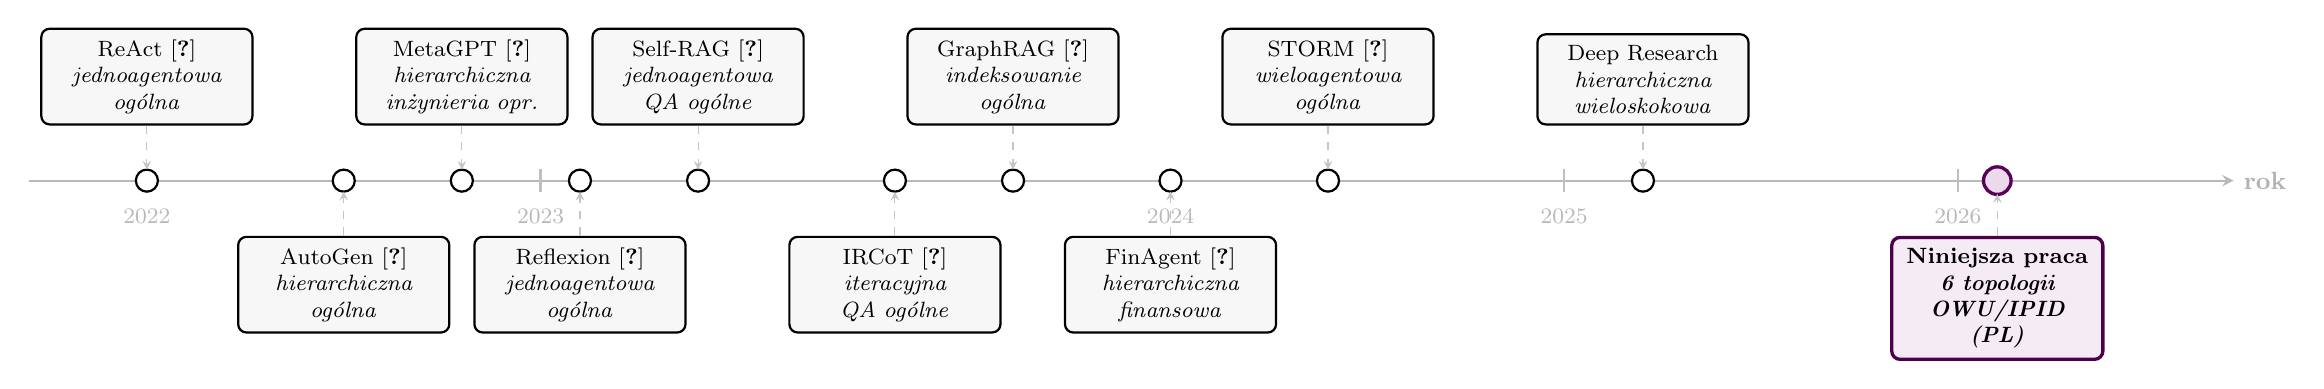
\begin{tikzpicture}[
        every node/.style={font=\small},
        dot/.style={circle, draw, thick, fill=white,
            minimum size=0.28cm, inner sep=0pt},
        dothighlight/.style={circle, draw=violet!70!black, very thick,
            fill=violet!15, minimum size=0.35cm, inner sep=0pt},
        workbox/.style={rectangle, draw, rounded corners=3pt, thick,
            text width=2.4cm, align=center, font=\footnotesize,
            fill=gray!6, inner sep=4pt},
        workboxhl/.style={rectangle, draw=violet!60!black, rounded corners=3pt,
            very thick, text width=2.4cm, align=center,
            font=\footnotesize\bfseries, fill=violet!8, inner sep=4pt},
        arrow/.style={->, >=stealth, thick, draw=gray!55},
        dasharrow/.style={->, >=stealth, dashed, thin, draw=gray!45}
      ]
      \draw[arrow] (-0.5, 0) -- (27.5, 0);
      \node[font=\small\bfseries, text=gray!60] at (27.9, 0) {rok};
      \foreach \x/\yr in {1.0/2022, 6.0/2023, 14.0/2024, 19.0/2025, 24.0/2026}{
          \draw[thick, gray!50] (\x, -0.15) -- (\x, 0.15);
          \node[font=\footnotesize, text=gray!55] at (\x, -0.45) {\yr};
        }
      \node[dot] at (1.0, 0) {};
      \node[workbox, above=0.7cm] (react) at (1.0, 0)
      {ReAct \cite{yao2022react}\\\textit{jednoagentowa\\ogólna}};
      \draw[dasharrow] (react.south) -- (1.0, 0.14);
      \node[dot] at (5.0, 0) {};
      \node[workbox, above=0.7cm] (metagpt) at (5.0, 0)
      {MetaGPT \cite{hong2023metagpt}\\\textit{hierarchiczna\\inżynieria opr.}};
      \draw[dasharrow] (metagpt.south) -- (5.0, 0.14);
      \node[dot] at (8.0, 0) {};
      \node[workbox, above=0.7cm] (selfrag) at (8.0, 0)
      {Self-RAG \cite{asai2023self}\\\textit{jednoagentowa\\QA ogólne}};
      \draw[dasharrow] (selfrag.south) -- (8.0, 0.14);
      \node[dot] at (3.5, 0) {};
      \node[workbox, below=0.7cm] (autogen) at (3.5, 0)
      {AutoGen \cite{wu2024autogen}\\\textit{hierarchiczna\\ogólna}};
      \draw[dasharrow] (autogen.north) -- (3.5, -0.14);
      \node[dot] at (6.5, 0) {};
      \node[workbox, below=0.7cm] (reflexion) at (6.5, 0)
      {Reflexion \cite{shinn2024reflexion}\\\textit{jednoagentowa\\ogólna}};
      \draw[dasharrow] (reflexion.north) -- (6.5, -0.14);
      \node[dot] at (12.0, 0) {};
      \node[workbox, above=0.7cm] (graphrag) at (12.0, 0)
      {GraphRAG \cite{edge2024local}\\\textit{indeksowanie\\ogólna}};
      \draw[dasharrow] (graphrag.south) -- (12.0, 0.14);
      \node[dot] at (16.0, 0) {};
      \node[workbox, above=0.7cm] (storm) at (16.0, 0)
      {STORM \cite{shao2024assisting}\\\textit{wieloagentowa\\ogólna}};
      \draw[dasharrow] (storm.south) -- (16.0, 0.14);
      \node[dot] at (14.0, 0) {};
      \node[workbox, below=0.7cm] (finagent) at (14.0, 0)
      {FinAgent \cite{zhang2024multimodal}\\\textit{hierarchiczna\\finansowa}};
      \draw[dasharrow] (finagent.north) -- (14.0, -0.14);
      \node[dot] at (10.5, 0) {};
      \node[workbox, below=0.7cm] (ircot) at (10.5, 0)
      {IRCoT \cite{trivedi2023interleaving}\\\textit{iteracyjna\\QA ogólne}};
      \draw[dasharrow] (ircot.north) -- (10.5, -0.14);
      \node[dot] at (20.0, 0) {};
      \node[workbox, above=0.7cm] (deepresearch) at (20.0, 0)
      {Deep Research\\\textit{hierarchiczna\\wieloskokowa}};
      \draw[dasharrow] (deepresearch.south) -- (20.0, 0.14);
      \node[dothighlight] at (24.5, 0) {};
      \node[workboxhl, below=0.7cm] (this) at (24.5, 0)
      {Niniejsza praca\\\textit{6 topologii\\OWU/IPID (PL)}};
      \draw[dasharrow] (this.north) -- (24.5, -0.17);
    \end{tikzpicture}
  \end{adjustbox}
  \zrodlo{opracowanie własne na podstawie literatury}
\end{figure}

\subsection{Luki badawcze i~wkład niniejszej pracy}\label{subsec:luki-badawcze-i-wklad-niniejszej-pracy}

Przegląd literatury ujawnia trzy wyraźne luki, które bezpośrednio motywują
projekt niniejszego badania. Żadna z~omówionych prac nie uwzględnia ich
wszystkich jednocześnie -- co oznacza, że mimo rozbudowanego dorobku w~obszarze
architektur agentowych i~systemów RAG, pytanie o~rzeczywisty wpływ topologii na
jakość odpowiedzi w~domenie regulacyjnej pozostaje otwarte.

Najistotniejszy jest brak kontrolowanych porównań wielu topologii przy stałym
modelu, tych samych narzędziach i~tym samym korpusie. W~każdej z~omówionych
prac trudno oddzielić wpływ topologii od wpływu lepszego wyszukiwania, bardziej
dopracowanych instrukcji systemowych lub innego modelu bazowego. Wang i~in.
oraz Xi i~in. wskazują ten brak jako jedną z~głównych przeszkód w~budowaniu
kumulatywnej wiedzy o~architekturach agentowych~\cite{wang2024survey,
  xi2025rise}. Nowa architektura zestawiana jest zazwyczaj z~prostym modelem
bazowym -- nie z~innymi architekturami w~identycznych warunkach -- co
uniemożliwia odpowiedź na pytanie, czy złożoność orkiestracji bezpośrednio
wpływa na wyższą jakość odpowiedzi, czy jedynie na wyższe koszty operacyjne.
Problem ten jest szczególnie widoczny, gdy wyniki poszczególnych prac są ze
sobą zestawiane: różnice w~modelu bazowym, zestawie narzędzi czy zbiorze
testowym sprawiają, że porównanie między architekturami opisywanymi w~różnych
publikacjach jest obarczone dużą niepewnością metodologiczną.

Drugą luką jest brak zestawu testowego dla dokumentów ubezpieczeniowych
w~języku polskim. Dostępne zbiory -- HotPotQA~\cite{yang2018hotpotqa},
Wikipedia, zadania programistyczne -- testują wnioskowanie wieloskokowe na
tekstach ogólnych i~nie obejmują problemów typowych dla tej domeny: sieci
wzajemnych odesłań między definicjami a~wyłączeniami, konieczności uzgadniania
sprzecznych postanowień czy porównywania zapisów z~wielu polis jednocześnie.
Polskojęzyczne zasoby ewaluacyjne dla tej dziedziny nie istnieją, co oznacza,
że wyniki uzyskane na zbiorach anglojęzycznych nie mogą być bezpośrednio
przeniesione na systemy operujące na polskich dokumentach regulacyjnych --
zarówno ze względu na różnice językowe, jak i~odmienną strukturę prawną.

Trzecia luka dotyczy głębokości analizy wyników. Dominujące podejście polega na
raportowaniu średnich wartości metryk jakościowych i~operacyjnych, co pozwala
co najwyżej uszeregować architektury według łącznego wyniku, lecz nie wyjaśnia
mechanizmów stojących za obserwowanymi różnicami. Wiedza o~tym, kiedy
i~dlaczego dany system zawodzi -- czy traci kontekst przy długich zadaniach,
czy błędnie klasyfikuje zapytania, czy propaguje błędy między modułami -- ma
bezpośrednią wartość przy wyborze architektury do zastosowania produkcyjnego.
Tymczasem analiza trybów niepowodzeń pozostaje w~literaturze nieobecna lub
ograniczona do kilku przykładów anegdotycznych.

Tabela~\ref{tab:zestawienie-prac-pokrewnych} zestawia omówione prace względem
tych trzech wymiarów. Każda ze zidentyfikowanych luk przekłada się bezpośrednio
na jeden z~wkładów badania: brak kontrolowanego porównania -- na projekt
eksperymentalny z~izolowaną topologią jako jedyną zmienną niezależną, przy
stałym modelu, narzędziach, korpusie i~zestawie 90~pytań dla wszystkich sześciu
architektur; brak polskiego zestawu testowego -- na oryginalny zestaw pytań
o~czterech poziomach trudności oparty wyłącznie na polskich dokumentach OWU
i~IPID, obejmujący zarówno pytania proste jak i~wymagające wieloetapowego
wnioskowania między sekcjami; brak analizy błędów -- na jakościowe badanie
śladów wykonania, które wykracza poza agregowane metryki i~pozwala
zidentyfikować wzorce niepowodzeń charakterystyczne dla każdej topologii wraz
z~rekomendacjami praktycznymi dla projektantów systemów produkcyjnych.

\begin{sidewaystable}[htbp]
  \caption{Zestawienie prac pokrewnych}\label{tab:zestawienie-prac-pokrewnych}
  \centering
  \small
  \renewcommand{\arraystretch}{1.3}
  \begin{tabularx}{0.95\textheight}{@{} p{2.8cm} p{2.8cm} p{3.5cm} p{3.5cm} p{3.5cm} X @{}}
    \toprule
    \textbf{System}
     & \textbf{Topologia}
     & \textbf{Dziedzina}
     & \textbf{Kontrolowane porównanie}
     & \textbf{Główna metryka}
     & \textbf{Luka względem niniejszej pracy}                                                        \\
    \midrule
    ReAct~\cite{yao2022react}
     & Jednoagentowa                                                      & Ogólna (Wikipedia)
     & Nie -- porównanie z~CoT                                            & Dokładność zadań
     & Brak domeny regulacyjnej, jedna topologia                                                      \\
    \addlinespace
    AutoGen~\cite{wu2024autogen}
     & Hierarchiczna, grupowa                                             & Kodowanie, ogólna
     & Nie -- brak wspólnego korpusu                                      & Wskaźnik sukcesu zadania
     & Brak kontrolowanego środowiska, brak QA na dokumentach                                         \\
    \addlinespace
    MetaGPT~\cite{hong2023metagpt}
     & Hierarchiczna                                                      & Inżynieria oprogramowania
     & Nie -- porównanie z~bazowym LLM                                    & Poprawność kodu
     & Brak domeny dokumentowej, jedna topologia                                                      \\
    \addlinespace
    FinAgent~\cite{zhang2024multimodal}
     & Hierarchiczna                                                      & Dokumenty finansowe
     & Nie -- brak linii bazowej jednoagentowej                           & Zwrot z~inwestycji
     & Brak kontrolowanego porównania topologii, domena finansowa                                     \\
    \addlinespace
    Self-RAG~\cite{asai2023self}
     & Jednoagentowa                                                      & Ogólna (QA)
     & Nie -- porównanie z~RAG                                            & Wierność, dokładność
     & Jedna topologia, brak domeny regulacyjnej                                                      \\
    \addlinespace
    Reflexion~\cite{shinn2024reflexion}
     & Jednoagentowa                                                      & Ogólna
     & Nie -- jedna architektura                                          & Wskaźnik sukcesu
     & Brak porównania topologii, brak dokumentów prawnych                                            \\
    \addlinespace
    GraphRAG~\cite{edge2024local}
     & Wzbogacone indeksowanie                                            & Ogólna (teksty długie)
     & Nie -- porównanie z~RAG                                            & Jakość odpowiedzi
     & Brak porównania topologii agentowych, brak domeny ubezpieczeniowej                             \\
    \addlinespace
    \rowcolor{violet!6}
    \textbf{Niniejsza praca}
     & \textbf{Sześć topologii}                                           & \textbf{Polskie OWU/IPID}
     & \textbf{Tak -- stały model, korpus, metryki}
     & \textbf{Wierność, poprawność, opóźnienie, tokeny}
     & \textbf{Kontrolowane porównanie, polska domena ubezpieczeniowa,
         analiza trybów niepowodzeń, rekomendacje produkcyjne}                                 \\
    \bottomrule
  \end{tabularx}
  \zrodlo{opracowanie własne na podstawie literatury}
\end{sidewaystable}

\chapter{Metodologia}\label{chap:metodologia}

W~rozdziale opisano podejście badawcze przyjęte w~niniejszej pracy. Opis
obejmuje wybór metody badawczej, strukturę eksperymentu, materiał badawczy,
kryteria oceny, procedurę analizy wyników oraz zasady odtwarzalności. Rozdział
przedstawia sposób przełożenia założeń teoretycznych na kontrolowany plan
badawczy.

\section{Metoda badawcza}\label{sec:metoda-badawcza}

Główny problem badawczy dotyczy wpływu topologii systemu agentowego na jakość
odpowiedzi generowanych na podstawie dokumentów regulacyjnych. Jako podstawową
metodę badawczą przyjęto kontrolowany eksperyment porównawczy, w~którym
warianty systemu przetwarzały ten sam korpus, odpowiadały na identyczny zestaw
pytań i~podlegały ujednoliconej procedurze oceny.

Wybór metody pozwala na izolację sposobu orkiestracji agentów jako jedynej
badanej zmiennej. Zastosowanie odmiennych modeli, indeksów dokumentów lub
zestawów narzędzi uniemożliwiłoby przypisanie różnic w~wynikach wyłącznie
testowanej architekturze. Układ kontrolowany eliminuje wpływ czynników
pobocznych.

Alternatywne metody badawcze zestawiono
w~tabeli~\ref{tab:porownanie-metod-badawczych}. Studium przypadku pojedynczej
architektury uniemożliwia ocenę porównawczą. Analiza teoretyczna pomija wpływ
specyfiki korpusu i~parametrów sterowania na zachowanie modeli językowych.
Z~kolei ankieta ekspercka mierzy subiektywne oczekiwania, a~nie rzeczywiste
parametry działania systemów w~ustandaryzowanych warunkach.

\begin{table}[H]
  \caption{Porównanie metod badawczych}\label{tab:porownanie-metod-badawczych}
  \centering
  \small
  \begin{tabularx}{\textwidth}{@{} p{3.2cm} L L @{}}
    \toprule
    \textbf{Podejście}
    & \textbf{Przydatność}
    & \textbf{Ograniczenie}                                              \\
    \midrule
    Studium przypadku
    & Pozwala szczegółowo opisać jedną architekturę
    & Nie daje podstaw do porównania topologii                           \\
    \addlinespace
    Analiza teoretyczna
    & Ułatwia uporządkowanie pojęć i~oczekiwanych zależności
    & Nie uwzględnia zachowania modelu na konkretnym korpusie            \\
    \addlinespace
    Ankieta ekspercka
    & Może zebrać opinie praktyków lub użytkowników domenowych
    & Mierzy ocenę subiektywną, a~nie przebieg systemu                   \\
    \addlinespace
    Eksperyment porównawczy
    & Umożliwia pomiar jakości i~kosztu w~tych samych warunkach
    & Wymaga ścisłej kontroli konfiguracji i~jednolitego protokołu oceny \\
    \bottomrule
  \end{tabularx}
  \zrodlo{opracowanie własne}
\end{table}

\section{Projekt eksperymentu}\label{sec:projekt-eksperymentu}

Eksperyment polega na porównaniu sześciu topologii agentowych w~identycznym
środowisku zadaniowym. Zmienną różnicującą jest wyłącznie organizacja pracy
systemu, w~tym kolejność kroków, zakres autonomii, podział zadań oraz liczba
wywołań narzędzi.

\subsection{Zmienna niezależna}\label{subsec:zmienna-niezalezna}

Zmienną niezależną jest topologia orkiestracji systemu agentowego. Pojęcie to
oznacza sposób organizacji przepływu informacji, obejmujący m.in. przetwarzanie
sekwencyjne, dekompozycję problemu na podzadania, planowanie działań, wybór
specjalisty na podstawie klasyfikacji pytania oraz iteracyjną modyfikację
kroków w~zależności od wyników pośrednich.

Do eksperymentu wybrano sześć topologii: deterministyczną, planer--wykonawca,
router--specjalista, tablicową, hierarchiczną oraz ReAct. Zestaw dobrano tak,
aby obejmował zarówno architektury jednoagentowe, jak i~wieloagentowe, a~także
różne poziomy autonomii sterowania. Każda architektura musiała pozwalać na
implementację w~jednolitym środowisku bez wprowadzania dodatkowych,
specyficznych narzędzi. Umożliwiło to analizę wpływu orkiestracji na jakość
odpowiedzi.

Tabela~\ref{tab:prownanie-architektur-agentowych} zestawia oba typy architektur
w~kluczowych wymiarach projektowych, stanowiąc punkt odniesienia dla
interpretacji wyników eksperymentu w~\cref{chap:eksperyment-i-wyniki}.

\begin{table}[H]
  \caption{Porównanie architektur agentowych}\label{tab:prownanie-architektur-agentowych}
  \centering
  \small
  \renewcommand{\arraystretch}{1.4}
  \begin{tabularx}{\textwidth}{@{} l L L @{}}
    \toprule
    \textbf{Wymiar}
    & \textbf{Jednoagentowe}
    & \textbf{Wieloagentowe}                                              \\
    \midrule
    Złożoność wdrożenia
    & Niska -- jeden kontekst, jedna instrukcja systemowa,
    jeden punkt awarii
    & Wysoka -- wiele instrukcji systemowych, mechanizmy
    koordynacji, wiele potencjalnych punktów awarii                        \\
    \addlinespace
    Koszt operacyjny
    & Niski -- jedno lub kilka wywołań LLM na pytanie
    & Wysoki -- każdy agent generował osobne wywołania;
    narzut koordynacji zwiększał zużycie
    tokenów~\cite{wang2024survey}                                          \\
    \addlinespace
    Zarządzanie kontekstem
    & Scentralizowane -- wszystkie informacje w~jednym buforze kontekstu;
    ryzyko przekroczenia limitu przy złożonych
    zadaniach~\cite{yao2022react}
    & Rozproszone -- agenci wykorzystywali rozdzielone podzbiory
    informacji; ryzyko utraty danych podczas ich
    przekazywania~\cite{wu2024autogen}                                     \\
    \addlinespace
    Odporność na błąd
    & Błąd w~jednym kroku mógł być skorygowany
    w~kolejnej iteracji pętli
    & Błąd w~węźle nadrzędnym propagował się kaskadowo
    do kolejnych agentów~\cite{wang2024survey}                             \\
    \addlinespace
    Specjalizacja ról
    & Brak -- jeden agent obsługiwał całe zadanie
    & Możliwa -- każdy agent mógł mieć wyspecjalizowaną
    instrukcję, narzędzia i~filtry
    metadanych~\cite{hong2023metagpt}                                      \\
    \addlinespace
    Skalowalność zadań
    & Ograniczona rozmiarem okna kontekstowego
    i~pojemnością pojedynczego modelu
    & Wyższa -- dekompozycja zadania pozwalała przetwarzać
    fragmenty równolegle~\cite{wu2024autogen}                              \\
    \addlinespace
    Przewidywalność
    & Wysoka -- deterministyczny przepływ sterowania zapewnia
    powtarzalność wyników
    & Niższa -- złożoność koordynacji obniża powtarzalność
    odpowiedzi dla identycznych
    zapytań~\cite{wang2024survey}                                          \\
    \addlinespace
    Typowe zastosowanie
    & Pytania wymagające jednego źródła wiedzy,
    systemy z~wymogiem niskich opóźnień
    & Zadania wymagające specjalizacji dziedzinowej,
    złożone przepływy z~wieloma krokami                                    \\
    \bottomrule
  \end{tabularx}
  \zrodlo{opracowanie własne na podstawie literatury}
\end{table}

\subsection{Zmienne zależne}\label{subsec:zmienne-zalezne}

Zmienne zależne obejmują dwa wymiary: jakość odpowiedzi oraz koszt operacyjny.
Ich rozdzielenie wynika z~faktu, że jakość osiągnięta przy dużej liczbie
wywołań modelu stanowi odmienną wartość aplikacyjną niż jakość uzyskana
w~prostszym przebiegu.

Do wymiaru jakości należały: wierność względem pobranych źródeł, poprawność
względem odpowiedzi referencyjnej, zwięzłość oraz trafność pobranych
dokumentów. Do wymiaru operacyjnego należały: opóźnienie, zużycie tokenów,
liczba wywołań narzędzi, liczba iteracji oraz wskaźnik błędów wykonania. Dobór
tych zmiennych wynikał z~metryk omówionych w~części teoretycznej, zwłaszcza
w~kontekście ewaluacji systemów agentowych i~RAG.

\subsection{Warunki kontrolowane}\label{subsec:warunki-kontrolowane}

Utrzymano stałe: model językowy, parametry generacji, korpus dokumentów, indeks
wektorowy, zestaw narzędzi, zbiór pytań, format odpowiedzi oraz procedurę
ewaluacji. Jest to warunek konieczny do zapewnienia porównywalności wyników
i~eliminacji wpływu środowiska testowego na działanie systemu.

Temperaturę generacji ustawiono na zero. Zabieg ten minimalizuje losowość
odpowiedzi modelu i~wariancję między przebiegami, co pozwala przypisać
zaobserwowane różnice bezpośrednio badanym mechanizmom sterowania, a~nie
zmienności LLM.

\begin{table}[H]
  \caption{Zestawienie warunków kontrolowanych}\label{tab:zestawienie-warunkow-kontrolowanych}
  \centering
  \small
  \begin{tabularx}{\textwidth}{@{} p{3.75cm} L @{}}
    \toprule
    \textbf{Element}
    & \textbf{Znaczenie dla porównania}                                    \\
    \midrule
    Model i~parametry
    & Eliminowały wpływ różnej jakości modeli oraz różnej
    losowości odpowiedzi                                                    \\
    \addlinespace
    Korpus dokumentów
    & Zapewniał wspólną podstawę wiedzy dla wszystkich architektur         \\
    \addlinespace
    Indeks wektorowy
    & Utrzymywał jednakowy punkt wyjścia dla etapu wyszukiwania            \\
    \addlinespace
    Zestaw narzędzi
    & Dawał każdej topologii ten sam zakres możliwych działań              \\
    \addlinespace
    Zestaw pytań
    & Pozwalał porównywać odpowiedzi na identycznych przypadkach testowych \\
    \addlinespace
    Protokół ewaluacji
    & Ujednolicał sposób oceny odpowiedzi i~śladów wykonania               \\
    \bottomrule
  \end{tabularx}
  \zrodlo{opracowanie własne}
\end{table}

\subsection{Plan porównawczy}\label{subsec:plan-porownawczy}

Przyjęto pełny plan porównawczy w~układzie zapytanie--architektura. Każde
z~90~pytań zostało obsłużone przez wszystkie sześć topologii, generując łącznie
540~uruchomień. Taki model wewnątrzgrupowy eliminuje wpływ zróżnicowanej
trudności zapytań na wyniki poszczególnych topologii.

Analiza zagregowana definiuje ogólny profil architektury, natomiast analiza
przekrojowa (według poziomu trudności, ubezpieczyciela i~kategorii produktu)
weryfikuje stabilność wyników poszczególnych wariantów przy zmianie warunków
wejściowych.

\section{Materiał badawczy}\label{sec:material-badawczy}

Materiał badawczy składał się z~dwóch części: korpusu dokumentów oraz zestawu
pytań testowych. Korpus stanowił bazę wiedzy dla testowanych systemów,
natomiast zbiór pytań służył do ilościowego pomiaru jakości generowanych
odpowiedzi. Z~uwagi na brak publicznego benchmarku dla polskojęzycznych
dokumentów ubezpieczeniowych, oba komponenty opracowano autorsko.

Korpus obejmował 22~dokumenty ubezpieczeniowe pochodzące od trzech głównych
towarzystw ubezpieczeniowych: ERGO Hestia S.A., Powszechnego Zakładu
Ubezpieczeń S.A. oraz TUiR Warta S.A. Dla każdego ubezpieczyciela uwzględniono
trzy kategorie produktowe: ubezpieczenia komunikacyjne, mieszkaniowe
i~podróżne. W~korpusie znalazły się dwa typy dokumentów: OWU oraz IPID.

Dokumenty ubezpieczeniowe charakteryzują się cechami stanowiącymi wyzwanie dla
architektur RAG i~systemów agentowych: dużą objętością, sformalizowaną
strukturą, obecnością odniesień krzyżowych oraz wymogiem ścisłego rozróżniania
zakresu ochrony, warunków i~wyłączeń. Złożoność korpusu pozwala na wyraźniejsze
uwidocznienie różnic w~skuteczności poszczególnych topologii względem prostych
zbiorów testowych.

Tabela~\ref{tab:zestawienie-korpusu-dokumentow} przedstawia skład korpusu
według ubezpieczycieli.

\begin{table}[H]
  \caption{Zestawienie korpusu dokumentów}\label{tab:zestawienie-korpusu-dokumentow}
  \centering
  \small
  \begin{adjustbox}{max width=0.78\textwidth}
    \begin{tabular}{@{} l c c c @{}}
      \toprule
      \textbf{Ubezpieczyciel}
      & \textbf{Kategorie}
      & \textbf{OWU}
      & \textbf{IPID}                                  \\
      \midrule
      Hestia         & 3                  & 3           & 3           \\
      PZU            & 3                  & 3           & 3           \\
      Warta          & 3                  & 5           & 5           \\
      \midrule
      \textbf{Razem} & \textbf{9}         & \textbf{11} & \textbf{11} \\
      \bottomrule
    \end{tabular}
  \end{adjustbox}
  \zrodlo{opracowanie własne}
\end{table}

Zestaw testowy opracowany na podstawie analizy manualnej dokumentów obejmuje
90~pytań. Do każdego przypisano odpowiedź referencyjną oraz uzasadniający
fragment źródłowy. Umożliwia to zautomatyzowaną ewaluację zgodności wyników
oraz ręczną weryfikację przypadków brzegowych.

Zdefiniowano cztery poziomy trudności. Poziom bardzo prosty testuje podstawową
orientację w~specyfikacji produktu. Poziom prosty wymaga zlokalizowania
pojedynczej informacji bazowej. Poziom złożony narzuca konieczność integracji
warunku, wyjątku lub uzupełniającego fragmentu kontekstu. Z~kolei pytania
bardzo złożone wymuszają syntezę danych z~wielu nieciągłych fragmentów
dokumentu w~celu zbudowania pełnej odpowiedzi.

Zestaw zbalansowano według ubezpieczycieli (po 30~pytań). Trzy główne poziomy
trudności zawierają po 27~pytań, a~poziom bardzo prosty – 9~pytań. Taka
dystrybucja eliminuje ryzyko obciążenia wyników specyfiką pojedynczego dostawcy
lub typu produktu.

\begin{table}[H]
  \caption{Zestawienie rozkładu pytań}\label{tab:zestawienie-rozkladu-pytan}
  \centering
  \small
  \begin{adjustbox}{max width=0.74\textwidth}
    \begin{tabular}{@{} l c c c c @{}}
      \toprule
      \textbf{Poziom trudności}
      & \textbf{Hestia}
      & \textbf{PZU}
      & \textbf{Warta}
      & \textbf{Razem}                                            \\
      \midrule
      Bardzo proste  & 3               & 3           & 3           & 9           \\
      Proste         & 9               & 9           & 9           & 27          \\
      Złożone        & 9               & 9           & 9           & 27          \\
      Bardzo złożone & 9               & 9           & 9           & 27          \\
      \midrule
      \textbf{Razem} & \textbf{30}     & \textbf{30} & \textbf{30} & \textbf{90} \\
      \bottomrule
    \end{tabular}
  \end{adjustbox}
  \zrodlo{opracowanie własne}
\end{table}

Przykłady pytań z~każdego poziomu przedstawia
tabela~\ref{tab:zestawienie-przykladowych-pytan}. Ilustruje ona różnice
w~oczekiwanym nakładzie pracy systemu dla każdej kategorii pytań: od krótkiej
odpowiedzi informacyjnej po odpowiedź wymagającą uwzględnienia warunku
i~wyjątku.

\begin{table}[H]
  \caption{Zestawienie przykładowych pytań}\label{tab:zestawienie-przykladowych-pytan}
  \centering
  \small
  \begin{adjustbox}{max width=0.94\textwidth}
    \begin{tabularx}{0.94\textwidth}{@{} p{2.4cm} L L @{}}
      \toprule
      \textbf{Poziom}
      & \textbf{Pytanie}
      & \textbf{Odpowiedź referencyjna}                                   \\
      \midrule
      Bardzo prosty
      & Na jaki okres zawierana jest standardowo umowa Autocasco z~WARTA?
      & Standardowo umowy AC zawiera się na 12~miesięcy.                  \\
      \addlinespace
      Prosty
      & Na jaki okres może zostać zawarte ubezpieczenie PZU Wojażer?
      & Umowa może zostać zawarta na czas oznaczony od 1~dnia do 1~roku.  \\
      \addlinespace
      Złożony
      & Czy PZU Wojażer obejmuje koszty leczenia spowodowane epidemią?
      & Co do zasady nie, z~wyjątkiem kosztów dotyczących nagłego
      zachorowania na COVID-19, kwarantanny lub izolacji.                  \\
      \addlinespace
      Bardzo złożony
      & Czy w~ubezpieczeniu PZU Wojażer objęte są ochroną koszty
      leczenia chorób przewlekłych?
      & Z~ochrony wyłączone są koszty leczenia chorób przewlekłych,
      z~wyjątkiem zaostrzeń albo powikłań, a~za opłatą dodatkowej
      składki ochrona może zostać rozszerzona do 100\% sumy
      ubezpieczenia.                                                       \\
      \bottomrule
    \end{tabularx}
  \end{adjustbox}
  \zrodlo{opracowanie własne}
\end{table}

\section{Kryteria oceny}\label{sec:kryteria-oceny}

Kryteria oceny zdefiniowano tak, aby uwzględniały zarówno odpowiedź końcową,
jak i~ślad jej generowania. W~systemach agentowych analiza samego wyjścia jest
niewystarczająca do diagnostyki działania. Przykładowo, dwie architektury mogą
wygenerować poprawną odpowiedź, jednak jedna z~nich uzyska ją optymalną ścieżką
wywołań, a~druga wykona operacje nadmiarowe. Z~kolei niska jakość odpowiedzi
może wynikać m.in. z~błędów wyszukiwania, logiki sterującej lub wadliwej
syntezy informacji.

\subsection{Miary ilościowe}\label{subsec:miary-ilosciowe}

Miary ilościowe dobrano spośród metryk omówionych w~rozdziale teoretycznym.
Objęły one dwa obszary: jakość odpowiedzi i~koszt operacyjny. W~obszarze
jakości zastosowano wierność, poprawność względem odpowiedzi referencyjnej,
zwięzłość oraz trafność dokumentów. W~obszarze kosztu uwzględniono opóźnienie,
zużycie tokenów, liczbę wywołań narzędzi, liczbę iteracji oraz błędy wykonania.

Wierność określa stopień pokrycia odpowiedzi pobranymi dokumentami, co jest
kluczowe dla wykrywania halucynacji w~dziedzinie ubezpieczeniowej. Poprawność
względem referencji mierzy trafność merytoryczną niezależnie od formalnej
zgodności z~kontekstem. Zwięzłość weryfikuje użyteczność formatu wyjściowego,
a~trafność dokumentów diagnozuje skuteczność etapu wyszukiwania.

Miary operacyjne charakteryzowały praktyczny koszt działania architektury.
Zużycie tokenów przekładało się bezpośrednio na koszt wywołań modelu,
opóźnienie na czas obsługi żądania, a~liczba narzędzi i~iteracji na złożoność
przebiegu. Wskaźnik błędów wykonania określa niezawodność: wysoka średnia
jakość odpowiedzi traci znaczenie praktyczne w~przypadku wysokiej awaryjności
działania.

Tabela~\ref{tab:zestawienie-metryk-oceny} przedstawia zestawienie wszystkich
zastosowanych miar, ich przedmiot oceny oraz uzasadnienie doboru.

\begin{table}[H]
  \caption{Zestawienie metryk oceny}\label{tab:zestawienie-metryk-oceny}
  \centering
  \small
  \renewcommand{\arraystretch}{1.4}
  \begin{tabularx}{\textwidth}{@{} l l L L @{}}
    \toprule
    \textbf{Wymiar}
    & \textbf{Miara}
    & \textbf{Co oceniała}
    & \textbf{Dlaczego istotna}                                   \\
    \midrule
    \multirow{4}{*}{\centering Jakość}
    & Wierność
    & Czy twierdzenia w~odpowiedzi miały oparcie w~dokumentach
    & Wykrywała halucynacje -- kluczowe w~domenie regulacyjnej    \\
    \addlinespace
    & Poprawność
    & Zgodność z~odpowiedzią referencyjną
    & Oceniała trafność merytoryczną niezależnie od stylu         \\
    \addlinespace
    & Zwięzłość
    & Adekwatność długości do pytania
    & Zbyt rozbudowane odpowiedzi obniżały użyteczność            \\
    \addlinespace
    & Trafność dokumentów
    & Czy pobrane fragmenty były istotne
    & Lokalizowała błąd na etapie wyszukiwania                    \\
    \midrule
    \multirow{4}{*}{\centering Koszt}
    & Zużycie tokenów
    & Łączna liczba tokenów wejściowych i~wyjściowych
    & Bezpośredni wskaźnik kosztu wywołań API                     \\
    \addlinespace
    & Liczba wywołań narzędzi
    & Ile razy architektura odwoływała się do narzędzi
    & Różnicowała architektury o~stałej i~zmiennej liczbie kroków \\
    \addlinespace
    & Opóźnienie
    & Czas od pytania do odpowiedzi końcowej
    & Istotne dla zastosowań produkcyjnych                        \\
    \addlinespace
    & Wskaźnik błędów
    & Odsetek uruchomień zakończonych błędem wykonania
    & Mierzył niezawodność architektury                           \\
    \bottomrule
  \end{tabularx}
  \zrodlo{opracowanie własne}
\end{table}

\subsection{Miary jakościowe}\label{subsec:miary-jakosciowe}

Ocenę ilościową uzupełniono analizą jakościową przebiegów. Jej celem było
ustalenie, w~jaki sposób dana architektura dochodziła do odpowiedzi i~w~którym
miejscu najczęściej dochodziło do spadku jakości. Analizie podlegały pytanie,
pobrane fragmenty, kolejność wywołań narzędzi, ewentualne decyzje sterujące,
odpowiedź końcowa oraz odpowiedź referencyjna.

Analiza jakościowa identyfikuje mocne strony i~ograniczenia topologii
niewidoczne w~wartościach uśrednionych. Przykładowo, architektura o~wysokich
wynikach średnich może generować stały narzut obliczeniowy dla prostych pytań,
a~topologia szybka -- wykazywać niestabilność w~obsłudze zapytań złożonych.

Niepowodzenia klasyfikowano według etapu, na którym powstał problem.
Tabela~\ref{tab:zestawienie-kategorii-bledow} przedstawia przyjętą taksonomię.
Kategorie miały charakter analityczny: pojedynczy przebieg mógł zawierać więcej
niż jeden problem, jednak klasyfikacja według dominującej przyczyny ułatwiała
porównanie architektur.

\begin{table}[H]
  \caption{Zestawienie kategorii błędów}\label{tab:zestawienie-kategorii-bledow}
  \centering
  \small
  \begin{tabularx}{\textwidth}{@{} l L @{}}
    \toprule
    \textbf{Kategoria}
    & \textbf{Opis}                                                        \\
    \midrule
    Błąd wyszukiwania
    & Pobrane fragmenty nie zawierały informacji potrzebnych do odpowiedzi \\
    \addlinespace
    Błąd rozumowania
    & Dowody były dostępne, ale system wyciągał z~nich niepoprawny wniosek \\
    \addlinespace
    Błąd sterowania
    & Topologia wybrała niewłaściwą ścieżkę, rolę, plan albo moment
    zakończenia                                                             \\
    \addlinespace
    Błąd syntezy
    & Odpowiedź końcowa zniekształcała poprawnie pobrane informacje        \\
    \addlinespace
    Nadmiarowy przebieg
    & System wykonywał zbędne kroki, które podnosiły koszt bez poprawy
    jakości                                                                 \\
    \bottomrule
  \end{tabularx}
  \zrodlo{opracowanie własne}
\end{table}

\subsection{Protokół ewaluacji}\label{subsec:protokol-ewaluacji}

Ewaluację odpowiedzi prowadzono dwutorowo. Pierwszy tor stanowiła ocena
automatyczna z~wykorzystaniem modelu językowego w~roli sędziego. Model oceniał
odpowiedzi według zdefiniowanych kryteriów i~zwracał wyniki dla metryk jakości.
Drugi tor stanowiła kontrola autorska, obejmująca przegląd wyników, analizę
przypadków trudnych oraz klasyfikację typów niepowodzeń.

Ewaluacja LLM-as-a-judge automatyzuje pomiar i~skaluje go do 540~uruchomień,
zapewniając jednocześnie determinizm stosowania kryteriów wobec badanych
architektur. Wyniki te służą wyłącznie jako względne porównanie systemów
w~ramach oceny algorytmicznej, nie zaś absolutna weryfikacja poprawności
interpretacji prawnej dokumentów.

W~toku analizy uwzględniono ograniczenia ewaluacji automatycznej: preferencję
wobec długości tekstu, podatność na styl bazowy modelu oraz niedoskonałą
detekcję niuansów dziedzinowych. Wobec tego metryki ilościowe interpretowano
łącznie z~jakościową analizą konkretnych przebiegów wykonania systemu.

\section{Procedura badawcza}\label{sec:procedura-badawcza}

Procedura badawcza definiuje strukturę eksperymentu od preparacji danych do
syntezy wniosków. Kluczowym założeniem jest izolacja etapów generacji, oceny
oraz analizy w~celu wyeliminowania sprzężeń zwrotnych.

\subsection{Etapy eksperymentu}\label{subsec:etapy-eksperymentu}

Proces eksperymentalny obejmuje pięć faz. W~pierwszej przygotowano materiał
badawczy. W~drugiej zdefiniowano warianty architektur. Trzecia faza to
uruchomienie pełnego planu zapytanie--architektura. Faza czwarta obejmuje
ewaluację. Piąta faza to wielowymiarowa analiza wyników (ilościowa, jakościowa
oraz produkcyjna).

\begin{figure}[H]
  \caption{Etapy eksperymentu}\label{fig:etapy-eksperymentu}
  \centering
  \begin{adjustbox}{max width=\textwidth}
    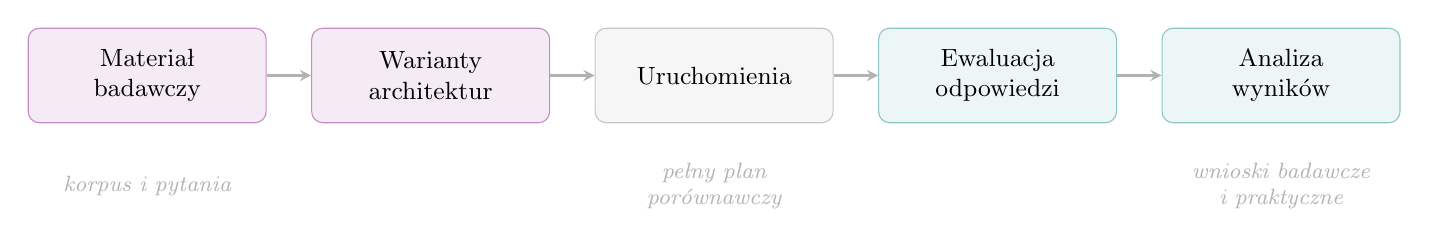
\begin{tikzpicture}[
        stepbox/.style={rectangle, draw, rounded corners=4pt,
          minimum width=2.8cm, minimum height=1.2cm,
          text width=2.6cm, align=center, text centered,
          inner sep=6pt, font=\small,
        fill=gray!7, draw=gray!45},
        arrow/.style={->, >=stealth, draw=gray!60, thick},
        lab/.style={font=\footnotesize\itshape, text=gray!60,
        align=center, text width=2.6cm}
      ]
      \node[stepbox, fill=violet!8, draw=violet!45] (s1) at (0,   0)
      {Materiał\\badawczy};
      \node[stepbox, fill=violet!8, draw=violet!45] (s2) at (3.6, 0)
      {Warianty\\architektur};
      \node[stepbox]                                (s3) at (7.2, 0)
      {Uruchomienia};
      \node[stepbox, fill=teal!7, draw=teal!45]     (s4) at (10.8,0)
      {Ewaluacja\\odpowiedzi};
      \node[stepbox, fill=teal!7, draw=teal!45]     (s5) at (14.4,0)
      {Analiza\\wyników};
      \draw[arrow] (s1) -- (s2);
      \draw[arrow] (s2) -- (s3);
      \draw[arrow] (s3) -- (s4);
      \draw[arrow] (s4) -- (s5);
      \node[lab] at (0,   -1.4) {korpus i~pytania};
      \node[lab] at (7.2, -1.4) {pełny plan\\porównawczy};
      \node[lab] at (14.4,-1.4) {wnioski badawcze\\i~praktyczne};
    \end{tikzpicture}
  \end{adjustbox}
  \zrodlo{opracowanie własne}
\end{figure}

Izolacja etapu ewaluacji zapobiega przekazywaniu informacji zwrotnej do
architektur generujących. Gwarantuje to, że każdy zarejestrowany przebieg jest
niezależnym i~obiektywnym wynikiem działania badanej topologii na przypisanym
pytaniu.

\subsection{Analiza ilościowa}\label{subsec:analiza-ilosciowa}

Analiza ilościowa realizowana jest dwupoziomowo. Poziom zagregowany obejmuje
wskaźniki uśrednione: jakość, koszt, opóźnienie, zużycie tokenów i~liczbę
błędów, definiujące ogólny profil efektywności każdej konfiguracji.

Poziom przekrojowy analizuje wyniki m.in. w~zależności od stopnia trudności
zapytania. Pozwala to zweryfikować korelację między złożonością topologii a~jej
skutecznością w~zadaniach wieloetapowych. Analiza przekrojowa eliminuje ponadto
ryzyko zaburzenia wyników przez lokalne ekstrema trudności w~poszczególnych
fragmentach korpusu.

Wnioski ilościowe są ograniczone do testowanej specyfiki i~nie stanowią
uniwersalnego benchmarku systemów agentowych. Ich zasadniczym celem jest
zmapowanie relacji między jakością a~kosztem na poziomie poszczególnych
topologii.

\subsection{Analiza jakościowa}\label{subsec:analiza-jakosciowa}

Analiza jakościowa koncentruje się na wybranych, brzegowych śladach wykonania:
przypadkach o~skrajnie niskiej ocenie, przerwaniach z~błędem oraz anomaliach
kosztowych. W~celu identyfikacji przyczyn niepowodzenia odtwarza się pełny ciąg
zdarzeń: od rozpoznania intencji do syntezy końcowej.

Badanie to ma na celu identyfikację wzorców błędów. Przykładowo,
w~architekturze router--specjalista weryfikuje się trafność klasyfikacji
zapytania; dla wariantów iteracyjnych -- celowość powtarzania kroków; dla
topologii zdecentralizowanych -- stabilność utrzymania danych w~toku przepływu
informacji.

Wyniki oceny jakościowej stanowią niezbędny kontekst dla metryk ilościowych,
umożliwiając odróżnienie architektur o~zbliżonej średniej, lecz odmiennych
klasach dominujących awarii.

\subsection{Perspektywa produkcyjna}\label{subsec:perspektywa-produkcyjna}

Ostatni wymiar analizy przekłada wyniki z~warunków kontrolowanych na środowisko
produkcyjne. Zdefiniowano w~nim granice uzasadnionej złożoności orkiestracji
oraz wskaźniki stabilności wdrożeniowej.

Wdrożenie komercyjne wymaga uwzględnienia przewidywalności, kosztu obsługi
i~ciągłości działania. Wobec tego wnioski z~eksperymentu przyjmują formę
rekomendacji wielokryterialnych, dostosowujących wybór architektury do wymagań
wierności, budżetu operacyjnego oraz przewidywanego stopnia złożoności systemu
produkcyjnego.

\section{Odtwarzalność}\label{sec:odtwarzalnosc}

Odtwarzalność jest jednym z~warunków wiarygodności eksperymentu. W~niniejszej
pracy miała ona istotne znaczenie, ponieważ badanie dotyczyło systemów opartych
na dużych modelach językowych, których zachowanie zależy od konfiguracji
modelu, wersji usług, sposobu przygotowania danych oraz treści promptów.

Odtwarzalność środowiska badawczego zabezpieczono przez pełną archiwizację
kodu, konfiguracji LLM, korpusów oraz logów ewaluacyjnych w~postaci zwartego
zestawu artefaktów. Takie ujęcie ustanawia referencyjny punkt odniesienia do
powtórnej weryfikacji obliczeń.

Z~racji zależności od zewnętrznych platform udostępniających modele przez API,
absolutna niezmienność wyników na poziomie generacji tokenów nie jest
gwarantowana. Jako środki zaradcze wprowadzono logowanie parametrów i~wersji
modeli w~repozytorium oraz udostępniono pełny zapis przebiegów, na których
bezpośrednio oparto wnioski badawcze.
\chapter{Implementacja}\label{chap:implementacja}

Rozdział opisuje platformę eksperymentalną zbudowaną na potrzeby porównania
sześciu architektur agentowych w~zadaniu odpowiadania na pytania dotyczące
polskich dokumentów ubezpieczeniowych. W~rozdziale omówiono stos
technologiczny, podział kodu na moduły, komponenty współdzielone przez
wszystkie warianty, implementację promptów, narzędzi agentowych i~grafów
sterowania, potok przetwarzania dokumentów, infrastrukturę ewaluacyjną oraz
wybrane decyzje inżynieryjne.

Kompletny kod źródłowy systemu, w~tym konfiguracja środowiska i~skrypty
eksperymentów, udostępniono w~publicznym repozytorium GitHub pod adresem
\url{https://github.com/mchojna/master-thesis-pjatk}.

Implementację oparto na założeniu metodologicznym, w~którym architektury różnią
się wyłącznie sposobem sterowania przebiegiem zadania. Dokumenty, indeks
wektorowy, zestaw narzędzi, konfiguracja modeli, format odpowiedzi i~procedura
ewaluacji są wspólne dla wszystkich wariantów. Podejście to determinuje
strukturę kodu, wymuszając wyraźną granicę między warstwą sterowania a~warstwą
operacyjną.

\section{Stos technologiczny}\label{sec:stos-technologiczny}

System zaimplementowano w~języku \texttt{Python} w~wersji 3.13. Warstwę
orkiestracji oparto na bibliotece \texttt{LangGraph}, umożliwiającej
definiowanie grafów stanowych z~węzłami asynchronicznymi, krawędziami
warunkowymi i~kontrolowanymi pętlami. Właściwości te są niezbędne do
odwzorowania różnic między topologiami. Dostęp do modeli językowych i~modelu
osadzeń zapewnia \texttt{LangChain} wraz z~pakietem \texttt{langchain-openai}.
Fragmenty dokumentów przechowywane są w~bazie wektorowej~\texttt{Qdrant},
a~warstwa ewaluacji i~rejestracji przebiegów korzysta z~\texttt{Arize Phoenix},
\texttt{PostgreSQL} oraz \texttt{OpenTelemetry}.

Tabela~\ref{tab:stos-technologiczny} zestawia komponenty stosu wraz z~wersjami
i~rolami w~systemie.

\begin{table}[H]
  \caption{Stos technologiczny}\label{tab:stos-technologiczny}
  \centering
  \small
  \begin{tabularx}{\textwidth}{@{} l l l L @{}}
    \toprule
    \textbf{Warstwa}
    & \textbf{Komponent}
    & \textbf{Wersja}
    & \textbf{Rola}                                                              \\
    \midrule
    Środowisko uruchomieniowe
    & \texttt{Python}                                           & \(\geq\)3.13
    & Język implementacji                                                        \\
    \addlinespace
    Orkiestracja agentów
    & \texttt{LangGraph}                                        & \(\geq\)0.2.0
    & Grafy stanowe architektur agentowych                                       \\
    \addlinespace
    Warstwa modeli językowych
    & \texttt{LangChain}, \texttt{langchain-openai}             & \(\geq\)1.2.10
    & Klienty modeli i~osadzeń                                                   \\
    & \texttt{OpenAI API}                                       & \(\geq\)2.21.0
    & Wywołania \texttt{gpt-5}, \texttt{text-embedding-3-large}                  \\
    & \texttt{Pydantic}                                         & \(\geq\)2.12.5
    & Schematy wyjść strukturalnych                                              \\
    \addlinespace
    Warstwa wyszukiwania
    & \texttt{Qdrant}                                           & 1.15
    & Baza wektorowa i~filtry metadanych                                         \\
    \addlinespace
    Warstwa ewaluacji
    & \texttt{Arize Phoenix}                                    & 13
    & Ewaluatory LLM-as-a-judge i~panel śledzenia                                \\
    & \texttt{PostgreSQL}                                       & 14
    & Baza operacyjna usługi \texttt{Phoenix}                                    \\
    \addlinespace
    Przetwarzanie dokumentów
    & \texttt{pypdfium2}, \texttt{Pillow}                       & \(\geq\)5.4.0
    & Renderowanie stron PDF do obrazów PNG                                      \\
    & \texttt{langchain-text-splitters}                         & \(\geq\)1.1.0
    & Fragmentacja Markdown po nagłówkach i~rekurencyjna                         \\
    \addlinespace
    Infrastruktura pomocnicza
    & \texttt{tenacity}, \texttt{structlog}                     & \(\geq\)9.1.4
    & Ponowienia wywołań i~logowanie strukturalne                                \\
    \bottomrule
  \end{tabularx}
  \zrodlo{opracowanie własne na podstawie pliku \texttt{pyproject.toml}}
\end{table}

W~systemie wyróżniono trzy klasy artefaktów. Danymi wejściowymi są pliki PDF
z~dokumentami OWU i~IPID oraz plik CSV z~pytaniami testowymi. Artefaktami
pośrednimi są pliki Markdown powstałe po ekstrakcji i~kolekcja \texttt{Qdrant}.
Artefaktami końcowymi są odpowiedzi agentów, metadane wykonania oraz pliki
ewaluacyjne. Tabela~\ref{tab:artefakty-systemu} zestawia wszystkie klasy
artefaktów z~ich lokalizacją i~zastosowaniem.

\begin{table}[H]
  \caption{Artefakty systemu}\label{tab:artefakty-systemu}
  \centering
  \small
  \begin{tabularx}{\textwidth}{@{} l L L @{}}
    \toprule
    \textbf{Etap}
    & \textbf{Artefakt}
    & \textbf{Zastosowanie}                                              \\
    \midrule
    \multirow{2}{*}{Wejście}
    & \texttt{data/documents/raw\_documents}
    & Surowe dokumenty OWU i~IPID w~formacie PDF                         \\
    & \texttt{data/evaluation/questions/*.csv}
    & Pytania, odpowiedzi referencyjne i~metadane próbek                 \\
    \addlinespace
    \multirow{3}{*}{Pośredni}
    & \texttt{data/documents/extracted\_documents}
    & Dokumenty po ekstrakcji do Markdown                                \\
    & \texttt{data/documents/insurance\_documents}
    & Kolekcja \texttt{Qdrant} z~wektorami i~metadanymi fragmentów       \\
    & \texttt{data/diagrams}
    & Diagramy architektur generowane z~definicji \texttt{Mermaid}       \\
    \addlinespace
    \multirow{2}{*}{Wyjście}
    & \texttt{data/evaluation/results/runner\_results\_*.jsonl/csv/json}
    & Surowe odpowiedzi, cytowania i~metadane wykonania                  \\
    & \texttt{data/evaluation/results/overall\_*\_*.csv}
    & Artefakty ewaluacji odpowiedzi i~trafności dokumentów              \\
    \bottomrule
  \end{tabularx}
  \zrodlo{opracowanie własne}
\end{table}

\section{Architektura modułowa systemu}\label{sec:architektura-modulowa-systemu}

Główna implementacja systemu mieści się w~module \texttt{sources} i~dzieli się
na sześć warstw: konfigurację, architektury agentowe, narzędzia, potok
dokumentów, wykonanie eksperymentu oraz narzędzia pomocnicze. Podział ten
ogranicza zależności między komponentami -- wymiana jednej architektury nie
wymaga modyfikacji narzędzi wyszukiwania, syntezy ani ewaluacji.

Istotny podział wprowadzono między katalogami \texttt{agents} i~\texttt{tools}.
Pierwszy z~nich zawiera wyłącznie logikę sterowania: kolejność węzłów,
krawędzie warunkowe, pętle i~warunki zakończenia. Drugi z~kolei zawiera
operacje dziedzinowe wykonywane przez wszystkie architektury: parsowanie
pytania, przepisywanie zapytania, wyszukiwanie, selekcję dowodów, cytowania,
dobór promptu i~syntezę odpowiedzi. Żadna z~architektur nie implementuje
własnej logiki wyszukiwania ani generowania odpowiedzi.

Zależności między warstwami przedstawiono na rysunku~\ref{fig:warstwy-systemu},
a~odpowiedzialności poszczególnych modułów opisano
w~tabeli~\ref{tab:moduly-systemu}.

\begin{figure}[H]
  \caption{Warstwy systemu}\label{fig:warstwy-systemu}
  \centering
  \begin{adjustbox}{max width=0.96\textwidth}
    \begin{tikzpicture}[
        block/.style={rectangle, draw, rounded corners=4pt,
          minimum height=2.5cm, text width=5.5cm,
        align=center, font=\footnotesize},
      ]
      \node[block, fill=violet!8, draw=violet!45] at (0, 0)
      {\textbf{\texttt{runner / evaluator / observer}}\\
      uruchomienia, ewaluacja, śledzenie};

      \node[block, fill=gray!10, draw=gray!45] at (6.5, 0)
      {\textbf{\texttt{agents}}\\
      sześć grafów \texttt{LangGraph} i~fabryka architektur};

      \node[block, fill=violet!5, draw=violet!30] at (13, 0)
      {\textbf{\texttt{tools}}\\
      wspólny rejestr ośmiu narzędzi agentowych};

      \node[block, fill=teal!6, draw=teal!35] at (0, -3.5)
      {\textbf{\texttt{extractor / chunker / vectorstore}}\\
      przygotowanie Markdown, fragmentów i~kolekcji \texttt{Qdrant}};

      \node[block, fill=teal!7, draw=teal!45] at (6.5, -3.5)
      {\textbf{\texttt{config}}\\
      ustawienia, prompty, klienty};

      \node[block, fill=teal!7, draw=teal!45] at (13, -3.5)
      {\textbf{\texttt{utilities}}\\
      metryki, diagramy};

    \end{tikzpicture}
  \end{adjustbox}
  \zrodlo{opracowanie własne}
\end{figure}

\begin{table}[H]
  \caption{Moduły systemu}\label{tab:moduly-systemu}
  \centering
  \small
  \begin{tabularx}{\textwidth}{@{} l L L @{}}
    \toprule
    \textbf{Moduł}
    & \textbf{Zakres}
    & \textbf{Główne pliki}                                     \\
    \midrule
    Konfiguracja
    & Konfiguracja ścieżek, modeli, \texttt{Qdrant},
    ewaluacji i~promptów
    & \texttt{app.py}, \texttt{graph.py}, \texttt{prompts.py}   \\
    Agenty
    & Implementacje sześciu topologii i~wspólny stan
    & \texttt{state.py}, \texttt{factory.py}, pliki architektur \\
    Narzędzia
    & Rejestr i~implementacja narzędzi agentowych
    & osiem modułów narzędziowych.                              \\
    Potok dokumentów
    & Ekstrakcja PDF, fragmentacja i~indeksowanie
    & \texttt{extractor.py}, \texttt{chuncker.py},
    \texttt{vectorstore.py}                                      \\
    Wykonanie
    & Uruchamianie macierzy pytań i~architektur
    & \texttt{runner.py}                                        \\
    Ewaluacja
    & Przygotowanie danych dla \texttt{Phoenix} i~zapis metryk
    & \texttt{evaluator.py}, \texttt{observer.py}               \\
    Pomocnicze
    & Śledzenie kosztów, tokenów i~renderowanie diagramów
    & \texttt{tracker.py},
    \texttt{drawer.py}                                           \\
    Notatniki
    & Sterowany przebieg przygotowania indeksu,
    uruchomień i~ewaluacji
    & \texttt{NB\_00} -- \texttt{NB\_04}                        \\
    \bottomrule
  \end{tabularx}
  \zrodlo{opracowanie własne}
\end{table}

\section{Elementy architektury współdzielone}\label{sec:elementy-architektury-wspoldzielone}

Komponenty współdzielone stanowią podstawę wszystkich architektur. Obejmują
wspólny obiekt stanu, konfigurację uruchomieniową, zamknięte schematy wyjść
strukturalnych, rejestr narzędzi oraz fabrykę grafów.
\subsection{Stan grafu}\label{subsec:stan-grafu}

Węzły grafów komunikują się za pomocą typowanego słownika
\texttt{ExperimentState}, zdefiniowanego w~\texttt{sources/agents/state.py}.
Każdy węzeł otrzymuje pełny stan, ale zwraca wyłącznie pola zmodyfikowane --
\texttt{LangGraph} scala je automatycznie. Zapobiega to nadpisywaniu wyników
poprzednich kroków i~upraszcza diagnostykę.

\begin{lstlisting}[language=Python,
  caption={Inicjalizacja stanu grafu},
  label={lst:inicjalizacja-stanu-grafu}]
def make_initial_state(
    question: str,
    pattern_name: str,
    *,
    company: str | None = None,
    product: str | None = None,
) -> dict:
    return {
        "question":          question,
        "company":           company,
        "product":           product,
        "intent":            None,
        "entities":          [],
        # ... (pola pomocnicze pominięte dla zwięzłości)
        "rewritten_queries": [],
        "retrieved_chunks":  [],
        "evidence_chunks":   [],
        "citations":         [],
        "answer":            None,
        "error":             None,
        "pattern_name":      pattern_name,
        "metadata":          {},
    }
\end{lstlisting}

Pola stanu pogrupowano według funkcji w~tabeli~\ref{tab:stan-grafu}. Pola
pomocnicze, specyficzne dla danej architektury (np. \texttt{\_plan},
\texttt{\_worker\_index}, \texttt{\_bb\_iter}, \texttt{\_react\_observations}),
przechowywane są w~słowniku \texttt{metadata}. Prefiks w~postaci podkreślenia
oznacza, że pole służy sterowaniu lokalnemu i~nie należy do kontraktu danych
eksperymentalnych.

\begin{table}[H]
  \caption{Stan grafu}\label{tab:stan-grafu}
  \centering
  \small
  \begin{tabular}{@{} l p{7cm} @{}}
    \toprule
    \textbf{Grupa}
    & \textbf{Pola}                                             \\
    \midrule
    Wejście
    & \texttt{question}, \texttt{pattern\_name},
    opcjonalnie \texttt{company}, \texttt{product}               \\
    Interpretacja pytania
    & \texttt{intent}, \texttt{entities},
    \texttt{is\_multi\_part}, \texttt{language}                  \\
    Wyszukiwanie
    & \texttt{rewritten\_queries}, \texttt{retrieved\_chunks},
    \texttt{evidence\_chunks}                                    \\
    Generowanie
    & \texttt{selected\_prompt\_template},
    \texttt{system\_prompt}, \texttt{citations}                  \\
    Odpowiedź
    & \texttt{answer\_body}, \texttt{answer\_with\_references},
    \texttt{answer}                                              \\
    Diagnostyka
    & \texttt{error}, \texttt{metadata}                         \\
    \bottomrule
  \end{tabular}
  \zrodlo{opracowanie własne}
\end{table}

\subsection{Konfiguracja uruchomieniowa}\label{subsec:konfiguracja-uruchomieniowa}

Konfiguracja składa się z~dwóch poziomów. \texttt{AppConfig}
z~\texttt{sources/config/app.py} to obiekt \texttt{Pydantic} agregujący grupy
ustawień: ścieżki danych, konfigurację modeli z~temperaturą \(0{,}0\),
parametry osadzeń, profile fragmentacji dla OWU i~IPID, parametry
\texttt{Qdrant} i~współbieżność. Mapa \texttt{role\_models} przypisuje modele
do ról pomocniczych i~głównej syntezy odpowiedzi.

\texttt{GraphConfig} z~\texttt{sources/config/graph.py} to stała
klasa danych, tworzona dla każdego przebiegu. Pełni rolę kontenera
zależności: udostępnia klienty modeli i~bazy wektorowej, inicjowane na żądanie
i~buforowane. Zapewnia to współdzielenie puli połączeń
HTTP w~ramach jednego przebiegu. Metoda \texttt{aclose} zamyka połączenia po jego zakończeniu,
co zapobiega wyczerpaniu puli przy 540 równoległych wywołaniach.

\subsection{Schematy wyjść strukturalnych}\label{subsec:schematy-wyjsc-strukturalnych}

W~\texttt{sources/config/schemas.py} zdefiniowano trzy schematy
\texttt{Pydantic} dziedziczące po \texttt{\_StrictBaseModel} z~atrybutem
\texttt{extra=``forbid''}. Są one przekazywane do API \texttt{OpenAI} za pomocą
interfejsu \texttt{with\_structured\_output}, co blokuje zwracanie
niezadeklarowanych pól.

\texttt{QuestionParseResult} opisuje wynik parsowania pytania: intencję
(dziewięć literałów), listę encji, flagę wieloczęściowości i~język.
\texttt{RouterDecision} ogranicza wyjście routera do ośmiu intencji
(z~pominięciem \texttt{unknown}), wymuszając jednoznaczną decyzję. \texttt{ReactDecision}
zawiera uzasadnienie, nazwę akcji i~parametry wyszukiwania.
Zamknięte schematy zapobiegają wystąpieniu nieoczekiwanych kluczy w~zmiennych
sterujących.

\subsection{Rejestr narzędzi i~fabryka grafów}\label{subsec:rejestr-narzedzi-i-fabryka-grafow}

Rejestr narzędzi w~\texttt{sources/tools/\_\_init\_\_.py} mapuje nazwy używane
przez agentów na asynchroniczne funkcje narzędziowe. Z~tego samego rejestru
korzystają architektura planer--wykonawca i~ReAct.

\begin{lstlisting}[language=Python,
  caption={Rejestr narzędzi agentowych},
  label={lst:rejestr-narzedzi-agentowych}]
TOOL_REGISTRY = {
    "question_parser":    parse_question,
    "query_rewriter":     rewrite_query,
    "retriever":          retrieve,
    "reranker":           rerank,
    "evidence_selector":  select_evidence,
    "citation_maker":     make_citations,
    "prompt_selector":    select_prompt,
    "answer_synthesizer": synthesize_answer,
}
\end{lstlisting}

Fabryka grafów w~\texttt{sources/agents/factory.py} powiązuje nazwę
architektury z~modułem udostępniającym funkcję \texttt{build\_graph}. Lista
\texttt{ALL\_PATTERNS} wykorzystywana jest przez komponent \texttt{runner} do
budowy macierzy uruchomień. Funkcja \texttt{build\_graph} wykorzystuje
\texttt{importlib} do importu odroczonego (ładowane są tylko moduły używane
w~uruchomieniu). Przekazanie nieznanej nazwy zgłasza \texttt{ValueError},
zapobiegając błędom braku obsługi danej topologii.

\section{Implementacja promptów}\label{sec:implementacja-promptow}

Wszystkie prompty zdefiniowano w~jednym module
\texttt{sources/config/prompts.py}. Taka centralizacja ułatwia kontrolę nad
systemem: instrukcje nie są rozproszone, a~każdy prompt ma jednoznaczną nazwę
i~miejsce użycia. Wyróżniono cztery grupy promptów: ekstrakcyjne, strukturalne,
sterujące i~odpowiedziowe. Dodatkową grupę stanowią prompty ewaluacyjne,
wykorzystywane przez usługę \texttt{Phoenix} po zakończeniu przebiegów. Pełne
treści promptów zamieszczono w~dodatku~\ref{app:prompty}.

\subsection{Prompt ekstrakcyjny}\label{subsec:prompt-ekstrakcyjny}

\texttt{EXTRACTION\_PROMPT} wykorzystywany jest podczas konwersji strony
PDF do formatu Markdown. Instrukcja wymusza zachowanie polskich znaków,
hierarchii nagłówków, numeracji, tabel i~list. W~przypadku dokumentów IPID
narzuca zestaw nagłówków drugiego poziomu, zgodny z~obowiązkowym układem
formularza. Dla dokumentów OWU wymaga zachowania struktury rozdziałów
i~paragrafów oraz odwzorowania tabel składek i~limitów. W~obu przypadkach
dodawanie treści nieobecnych w~źródle jest zabronione, co ogranicza ryzyko
halucynacji na etapie ekstrakcji.

\subsection{Prompty strukturalne}\label{subsec:prompty-strukturalne}

Prompty strukturalne zwracają dane w~formacie JSON, przetwarzane następnie
przez kod sterujący. Parser pytania i~router wykorzystują
\texttt{with\_structured\_output} oraz schematy \texttt{Pydantic}. Pozostałe
prompty zwracają tablice JSON, parsowane ręcznie z~wykorzystaniem mechanizmu
awaryjnego.

\texttt{QUERY\_REWRITER\_SYSTEM\_PROMPT} generuje trzy warianty zapytania:
bezpośredni, uogólniony i~hipotetyczny (implementujący strategię HyDE).
\texttt{RERANKER\_SYSTEM\_PROMPT} ocenia trafność fragmentów w~partiach.
\texttt{ROUTER\_SYSTEM\_PROMPT} klasyfikuje pytanie do jednej z~ośmiu intencji.
\texttt{PLANNER\_SYSTEM\_PROMPT} buduje plan z~maksymalnie ośmioma krokami.
\texttt{REACT\_SYSTEM\_PROMPT} prowadzi pojedynczą iterację cyklu
myśl--akcja--obserwacja. \texttt{DECOMPOSER\_SYSTEM\_PROMPT} dzieli pytanie
złożone na maksymalnie trzy podpytania.

\subsection{Prompty odpowiedziowe}\label{subsec:prompty-odpowiedziowe}

Słownik \texttt{PROMPT\_TEMPLATES} przypisuje szablony odpowiedzi do jedenastu
intencji pytań. Wszystkie szablony wymuszają strukturę złożoną z~sekcji
\textbf{Odpowiedź} (krótka konkluzja), separatora oraz sekcji
\textbf{Szczegóły} (uzasadnienie z~obowiązkiem cytowania każdego faktu
znacznikiem \texttt{[N]}). Szablony różnią się strategią wyboru fragmentów:
\texttt{EXCLUSIONS\_PROMPT} dotyczy wyłączeń, \texttt{LIMITS\_PROMPT} -- sum
ubezpieczenia, \texttt{CLAIMS\_PROMPT} -- procedury zgłoszenia szkody,
a~\texttt{COMPARISON\_PROMPT} narzuca układ tabelaryczny. We wszystkich
wariantach zalecono zwięzłość i~neutralny ton w~języku polskim.

\subsection{Prompty ewaluacyjne}\label{subsec:prompty-ewaluacyjne}

Komponent ewaluacyjny \texttt{Phoenix} wykorzystuje instrukcje
\texttt{REFERENCE\_CORRECTNESS\_PROMPT} i~\texttt{CONCISENESS\_PROMPT} po
zakończeniu przebiegów. Każdy prompt definiuje pięciostopniową skalę ocen (od 1
do 5). Oddzielenie promptów generujących od oceniających zapobiega przeciekowi
informacji między warstwami.

Tabela~\ref{tab:prompty-systemu} zestawia wszystkie grupy promptów z~ich
zastosowaniem.

\begin{table}[H]
  \caption{Prompty systemu}\label{tab:prompty-systemu}
  \centering
  \small
  \begin{tabularx}{\textwidth}{@{} l L L @{}}
    \toprule
    \textbf{Grupa}
    & \textbf{Prompty}
    & \textbf{Zastosowanie}                            \\
    \midrule
    Ekstrakcja
    & \texttt{EXTRACTION\_PROMPT}
    & Konwersja stron PDF do Markdown                  \\
    Strukturalne
    & \texttt{QUESTION\_PARSER\_SYSTEM\_PROMPT},
    \texttt{QUERY\_REWRITER\_SYSTEM\_PROMPT},
    \texttt{RERANKER\_SYSTEM\_PROMPT}
    & Dane dla filtrów, zapytań i~oceny fragmentów     \\
    Sterujące
    & \texttt{PLANNER\_SYSTEM\_PROMPT},
    \texttt{ROUTER\_SYSTEM\_PROMPT},
    \texttt{REACT\_SYSTEM\_PROMPT},
    \texttt{DECOMPOSER\_SYSTEM\_PROMPT},
    \texttt{MERGE\_ANSWERS\_SYSTEM\_PROMPT}
    & Decyzje grafów i~łączenie odpowiedzi częściowych \\
    Odpowiedziowe
    & \texttt{FAQ\_PROMPT}, \texttt{COVERAGE\_PROMPT},
    \texttt{EXCLUSIONS\_PROMPT}, \texttt{LIMITS\_PROMPT},
    \texttt{COMPARISON\_PROMPT}, \texttt{CLAIMS\_PROMPT}
    i~pięć pozostałych
    & Dobór stylu odpowiedzi do intencji pytania       \\
    Ewaluacyjne
    & \texttt{REFERENCE\_CORRECTNESS\_PROMPT},
    \texttt{CONCISENESS\_PROMPT}
    & Ocena odpowiedzi po zakończeniu przebiegu        \\
    \bottomrule
  \end{tabularx}
  \zrodlo{opracowanie własne}
\end{table}

\section{Implementacja narzędzi}\label{sec:implementacja-narzedzi}

Narzędzia agentowe zrealizowano jako funkcje asynchroniczne o~wspólnym
kontrakcie: przyjmują bieżący stan \texttt{ExperimentState} oraz konfigurację
\texttt{GraphConfig}, a~zwracają słownik częściowej aktualizacji stanu.
Umożliwia to wywoływanie tych samych narzędzi z~poziomu grafu liniowego, pętli
wykonawcy, dyspozytora tablicowego oraz kontrolera ReAct.

\begin{lstlisting}[language=Python,
  caption={Kontrakt narzędzia agentowego},
  label={lst:kontrakt-narzedzia-agentowego}]
async def tool_name(
    state: ExperimentState,
    *,
    config: GraphConfig,
    **kwargs,
) -> dict:
    ...
\end{lstlisting}

Każde narzędzie aktualizuje słownik \texttt{metadata}:
\texttt{record\_tool\_call} rejestruje liczbę i~kolejność wywołań, natomiast
\texttt{record\_model\_usage} dopisuje szacowaną liczbę tokenów i~koszt
operacji. Metadane te służą analizie przebiegu i~nie wpływają na zwracaną
odpowiedź.

\subsection{Parser pytania}\label{subsec:parser-pytania}

Narzędzie \texttt{question\_parser} wyodrębnia z~pytania nazwę ubezpieczyciela,
produkt, intencję (spośród dziewięciu literałów), listę encji, flagę
\texttt{is\_multi\_part} i~język. Wywołanie zrealizowano za pomocą
\texttt{with\_structured\_output} oraz schematu \texttt{QuestionParseResult}.
W~przypadku błędu zwracany jest stan awaryjny z~intencją \texttt{unknown}, bez
przerywania przebiegu. Jeżeli zidentyfikowano produkt bez nazwy firmy, jest ona
uzupełniana na podstawie wewnętrznego mapowania.

\subsection{Przepisywanie zapytania}\label{subsec:przepisywanie-zapytania}

Narzędzie \texttt{query\_rewriter} generuje trzy warianty zapytania:
bezpośredni (zachowujący oryginalne słownictwo), uogólniony (wykorzystujący
nazwy sekcji dokumentów) i~hipotetyczny (realizujący strategię HyDE).
W~przypadku błędu parsowania zapytanie powielane jest w~trzech kopiach jako
bezpieczny wariant domyślny.

\subsection{Wyszukiwanie}\label{subsec:wyszukiwanie}

Narzędzie \texttt{retriever} wektoryzuje zapytanie i~odpytuje kolekcję
\texttt{Qdrant}. Przed konstrukcją filtra normalizowane są metadane: usuwane są
znaki diakrytyczne oraz rozwiązywane są aliasy. Wyszukiwanie wykorzystuje
trójstopniową relaksację filtrów: najpierw uwzględnia firmę i~produkt,
następnie wyłącznie firmę, a~na końcu przebiega bez filtra.

\begin{lstlisting}[language=Python,
  caption={Relaksacja filtrów wyszukiwania},
  label={lst:relaksacja-filtrow-wyszukiwania}]
for filter_mode, query_filter in _build_filter_candidates(
    parsed_company, parsed_product
):
    hits = await config.qdrant.query_points(
        collection_name=config.collection_name,
        query=query_vector,
        query_filter=query_filter,
        limit=retrieval_limit,
    )
    for point in hits.points:
        collected_points[str(point.id)] = point
    if len(collected_points) >= minimum_hits:
        break
\end{lstlisting}

Funkcja \texttt{retrieve\_multi} wykonuje \texttt{retriever} równolegle
(\texttt{asyncio.gather}) dla trzech wariantów zapytania. Wyniki podlegają
deduplikacji względem klucza \texttt{(source\_file, header\_2, header\_3)},
a~zachowywany jest fragment o~najwyższym podobieństwie.

\subsection{Ponowne szeregowanie}\label{subsec:ponowne-szeregowanie}

Narzędzie \texttt{reranker} ocenia trafność fragmentów z~wykorzystaniem modelu
językowego (funkcja domyślnie wyłączona). W~wariancie aktywnym dzieli fragmenty
na partie z~uwzględnieniem limitu tokenów, ocenia je współbieżnie i~odrzuca
wyniki poniżej progu \(0{,}3\). Węzeł zaimplementowano w~każdym grafie, co
umożliwia parametryzację eksperymentu.

\subsection{Selektor dowodów}\label{subsec:selektor-dowodow}

Narzędzie \texttt{evidence\_selector} to deterministyczna funkcja operująca bez
modelu językowego. Realizuje deduplikację względem pary \texttt{(source\_file,
header\_2)}, sortowanie (na podstawie wyniku, głębokości nagłówka i~długości
fragmentu), wybór najlepszych fragmentów (\texttt{evidence\_top\_k}) przy
zapewnieniu pokrycia co najmniej dwóch plików źródłowych oraz utrzymanie
stabilnej kolejności wyników.

\subsection{Generator cytowań}\label{subsec:generator-cytowan}

Narzędzie \texttt{citation\_maker} konstruuje listę cytowań z~wykorzystaniem
fragmentów dowodowych. Pojedyncze cytowanie obejmuje identyfikator, plik
źródłowy, typ dokumentu, metadane oraz cytat do 320 znaków. Numeracja cytowań
jest zachowywana podczas całego przebiegu, co gwarantuje spójność odnośników
\texttt{[N]} ze stopką \textbf{Źródła}.

\subsection{Selektor promptu}\label{subsec:selektor-promptu}

Narzędzie \texttt{prompt\_selector} określa szablon odpowiedzi na podstawie
zmiennej \texttt{intent} (wariant awaryjny to \texttt{unknown}). Decyzja
podejmowana jest w~sposób deterministyczny, co eliminuje wywołania modelu
językowego i~zużycie tokenów.

\subsection{Syntezator odpowiedzi}\label{subsec:syntezator-odpowiedzi}

Narzędzie \texttt{answer\_synthesizer} buduje blok kontekstu na podstawie
pytania, metadanych oraz cytowań, a~następnie wywołuje model z~wybranym
szablonem. Otrzymana odpowiedź podlega trójstopniowej normalizacji: wymuszeniu
formatu \textbf{Odpowiedź}/\textbf{Szczegóły}, standaryzacji znaczników oraz
dołączeniu stopki \textbf{Źródła}. Błąd API logowany jest w~zmiennej
\texttt{error}, a~zwracany komunikat informuje o~niewystarczającym kontekście.

Tabela~\ref{tab:narzedzia-agentowe} zestawia wszystkie narzędzia.

\begin{table}[H]
  \caption{Narzędzia agentowe}\label{tab:narzedzia-agentowe}
  \centering
  \small
  \begin{tabularx}{\textwidth}{@{} l L L c @{}}
    \toprule
    \textbf{Narzędzie}
    & \textbf{Wejście}
    & \textbf{Wyjście}
    & \textbf{Model}                             \\
    \midrule
    \texttt{question\_parser}
    & pytanie, opcjonalnie firma i~produkt
    & intencja, encje, firma, produkt, język
    & tak                                        \\
    \texttt{query\_rewriter}
    & pytanie i~metadane parsera
    & trzy warianty zapytania
    & tak                                        \\
    \texttt{retriever}
    & zapytanie, firma, produkt, \texttt{top\_k}
    & fragmenty z~\texttt{Qdrant}
    & osadzenia                                  \\
    \texttt{reranker}
    & pytanie i~fragmenty
    & przefiltrowane fragmenty z~wynikiem
    & tak                                        \\
    \texttt{evidence\_selector}
    & fragmenty pobrane lub ocenione
    & zwięzły zestaw dowodów
    & nie                                        \\
    \texttt{citation\_maker}
    & fragmenty dowodowe
    & obiekty cytowań
    & nie                                        \\
    \texttt{prompt\_selector}
    & intencja
    & nazwa szablonu i~prompt systemowy
    & nie                                        \\
    \texttt{answer\_synthesizer}
    & pytanie, dowody, cytowania, prompt
    & odpowiedź i~źródła
    & tak                                        \\
    \bottomrule
  \end{tabularx}
  \zrodlo{opracowanie własne}
\end{table}

\section{Implementacja architektur agentowych}\label{sec:implementacja-architektur-agentowych}

Każda architektura stanowi osobny moduł w~\texttt{sources/agents}, eksportujący
funkcję \texttt{build\_graph}. Funkcja ta tworzy graf
\texttt{StateGraph(ExperimentState)}, rejestruje węzły, definiuje krawędzie
i~zwraca skompilowany obiekt \texttt{LangGraph}. Diagramy architektur
wygenerowano automatycznie na podstawie definicji \texttt{Mermaid}
i~zamieszczono w~dodatku~\ref{app:diagramy}.

\subsection{Architektura deterministyczna}\label{subsec:architektura-deterministyczna}

Architektura deterministyczna to graf liniowy pozbawiony węzłów decyzyjnych.
Przetwarzanie pytania obejmuje sekwencję ośmiu kroków: parsowanie,
przepisywanie, wyszukiwanie wielozapytaniowe, ponowne szeregowanie, selekcję
dowodów, wybór promptu, budowę cytowań i~syntezę. Brak pętli i~warunków
sprawia, że wariant ten stanowi punkt odniesienia: profil kosztów jest
deterministyczny, a~wszelkie różnice względem pozostałych architektur wynikają
wyłącznie z~logiki sterującej.

\begin{lstlisting}[language=Python,
  caption={Krawędzie grafu deterministycznego},
  label={lst:krawedzie-grafu-deterministycznego}]
graph.add_edge(START,             "parse_question")
graph.add_edge("parse_question",  "rewrite_query")
graph.add_edge("rewrite_query",   "retrieve_all")
graph.add_edge("retrieve_all",    "rerank")
graph.add_edge("rerank",          "select_evidence")
graph.add_edge("select_evidence", "select_prompt")
graph.add_edge("select_prompt",   "make_citations")
graph.add_edge("make_citations",  "generate_answer")
graph.add_edge("generate_answer", END)
\end{lstlisting}

\subsection{Architektura planer--wykonawca}\label{subsec:architektura-planer-wykonawca}

Architektura planer--wykonawca wdraża węzeł planera poprzedzający wykonanie
narzędzi. Planer przetwarza pytanie i~definicje narzędzi
z~\texttt{TOOL\_REGISTRY}, zwracając listę kroków w~formacie JSON
(\texttt{\{tool\_name, rationale\}}). Walidacja planu wymaga maksymalnie ośmiu
kroków z~rejestru, zakończonych wywołaniem \texttt{answer\_synthesizer}. Błąd
parsowania lub niespełnienie warunków skutkuje przyjęciem planu awaryjnego
(zgodnego z~potokiem deterministycznym).

\begin{lstlisting}[language=Python,
  caption={Warunek pętli wykonawcy},
  label={lst:warunek-petli-wykonawcy}]
def should_continue(state: ExperimentState) -> str:
    metadata = state.get("metadata", {})
    plan = metadata.get("_plan", [])
    idx  = metadata.get("_plan_index", 0)
    if (idx < len(plan)
            and plan[idx].get("tool_name") != "answer_synthesizer"):
        return "executor"
    return "synthesizer"
\end{lstlisting}

\subsection{Architektura router--specjalista}\label{subsec:architektura-router-specjalista}

Architektura router--specjalista klasyfikuje pytanie do jednej z~ośmiu intencji
(schemat \texttt{RouterDecision}), a~następnie deleguje wykonanie do jednego
z~czterech podpotoków (FAQ, opis, roszczenia, porównania). Podpotoki
współdzielą zestaw kroków, różniąc się strategią wyszukiwania: wariant
roszczeniowy zwiększa parametr \texttt{top\_k}, wariant porównawczy omija filtr
firmy, a~wariant FAQ wykorzystuje pojedyncze zapytanie.

\begin{lstlisting}[language=Python,
  caption={Mapowanie intencji na podpotoki},
  label={lst:mapowanie-intencji-na-podpotoki}]
# app_config.router.category_to_pipeline
CATEGORY_TO_PIPELINE = {
    "faq":         "faq",
    "limits":      "faq",
    "description": "description",
    "coverage":    "description",
    "conditions":  "description",
    "claims":      "claims",
    "exclusions":  "claims",
    "comparison":  "comparison",
}
\end{lstlisting}

\subsection{Architektura tablicowa}\label{subsec:architektura-tablicowa}

W~architekturze tablicowej model językowy zastąpiono deterministyczną funkcją
regułową (dyspozytorem). W~kolejnych iteracjach dyspozytor weryfikuje
uzupełnienie pól stanu i~inicjuje odpowiednie narzędzie (przy stałej kolejności
weryfikacji). Po powrocie do dyspozytora inkrementowany jest licznik iteracji.
Parametr \texttt{max\_blackboard\_iterations} zapobiega wystąpieniu
nieskończonej pętli.

\begin{lstlisting}[language=Python,
  caption={Reguły dyspozytora tablicowego},
  label={lst:reguly-dyspozytora-tablicowego}]
if metadata.get("_bb_iter", 0) >= max_iter:
    return "answer_agent"
if state.get("intent") is None:
    return "parser_agent"
if not state.get("rewritten_queries"):
    return "rewriter_agent"
if not state.get("retrieved_chunks"):
    return "retriever_agent"
if chunks and not state.get("evidence_chunks"):
    return "evidence_selector_agent"
\end{lstlisting}

\subsection{Architektura hierarchiczna}\label{subsec:architektura-hierarchiczna}

Architektura hierarchiczna obejmuje cztery komponenty: parser, dekompozytor,
pętlę pracownika i~syntezator. Dekompozytor dzieli zapytanie (na maksymalnie
trzy podpytania). Pracownik przetwarza je w~uproszczonym potoku (przepisanie,
wyszukiwanie, selekcja, odpowiedź częściowa). Syntezator integruje wyniki,
wykonując globalną deduplikację cytowań i~wymuszając dwusekcyjny format.
Deduplikacja fragmentów zapobiega liniowemu przyrostowi rozmiaru kontekstu.

\begin{lstlisting}[language=Python,
  caption={Pętla pracownika w~architekturze hierarchicznej},
  label={lst:petla-pracownika-w-architekturze-hierarchicznej}]
def should_continue_worker(state: ExperimentState) -> str:
    metadata = state.get("metadata", {})
    idx = metadata.get("_worker_index", 0)
    sub = metadata.get("sub_questions", [])
    if idx < len(sub):
        return "worker"
    return "synthesizer"
\end{lstlisting}

\subsection{Architektura ReAct}\label{subsec:architektura-react}

Architektura ReAct integruje trzy węzły: agenta, wykonawcę narzędzi oraz węzeł
wymuszonego zakończenia. Agent iteracyjnie zwraca obiekt \texttt{ReactDecision}
(myśl, akcja, parametry). Wykonawca inicjuje narzędzie i~loguje skróconą
obserwację w~\texttt{\_react\_observations} (pomijając pełną treść odpowiedzi).
Zakończenie następuje po akcji \texttt{finish}, wygenerowaniu odpowiedzi lub
przekroczeniu limitu iteracji. Mechanizm skróconych obserwacji zapobiega
rozrostowi kontekstu.

\begin{lstlisting}[language=Python,
  caption={Warunek kontynuacji pętli ReAct},
  label={lst:warunek-kontynuacji-petli-react}]
def should_continue(state: ExperimentState) -> str:
    metadata   = state.get("metadata", {})
    decision   = metadata.get("_react_decision", {})
    iterations = len(metadata.get("_react_observations", []))
    if decision.get("action") == "finish" or state.get("answer") is not None:
        return "finish"
    if iterations >= max_iter:
        return "force_finish"
    return "agent"
\end{lstlisting}

Tabela~\ref{tab:zestawienie-topologii-grafow} zestawia implementacyjne różnice
między architekturami.

\begin{table}[H]
  \caption{Zestawienie topologii grafów}\label{tab:zestawienie-topologii-grafow}
  \centering
  \small
  \begin{tabularx}{\textwidth}{@{} l L L L @{}}
    \toprule
    \textbf{Architektura}
    & \textbf{Sterowanie}
    & \textbf{Cechy grafu}
    & \textbf{Zakończenie}                              \\
    \midrule
    Deterministyczna
    & Stała sekwencja
    & Liniowy, skierowany acykliczny graf, osiem węzłów
    & Ostatni węzeł                                     \\
    Planer--wykonawca
    & Plan JSON z~modelu
    & Planer, pętla wykonawcy, synteza
    & Wyczerpanie planu                                 \\
    Router--specjalista
    & Klasyfikacja intencji
    & Router i~cztery podpotoki
    & Koniec podpotoku                                  \\
    Tablicowa
    & Reguły na stanie
    & Dyspozytor i~pula agentów
    & Odpowiedź lub limit                               \\
    Hierarchiczna
    & Dekompozycja pytania
    & Dekompozytor, pętla, scalanie
    & Wszystkie podpytania                              \\
    ReAct
    & Decyzja modelu w~pętli
    & Agent, wykonawca, zakończenie
    & \texttt{finish} lub limit                         \\
    \bottomrule
  \end{tabularx}
  \zrodlo{opracowanie własne}
\end{table}

\section{Protokół przetwarzania dokumentów}\label{sec:protokol-przetwarzania-dokumentow}

Potok dokumentów przygotowuje zamknięty korpus do wyszukiwania wektorowego.
Proces ten uruchamiany jest jednorazowo przed eksperymentem (architektury nie
modyfikują go w~trakcie odpowiadania). Obejmuje cztery etapy: ekstrakcję PDF do
Markdown, fragmentację tekstu, wektoryzację oraz zapis w~\texttt{Qdrant}.
Kolejność operacji zilustrowano na
rysunku~\ref{fig:potok-przetwarzania-dokumentow}.

\begin{figure}[H]
  \caption{Potok przetwarzania dokumentów}\label{fig:potok-przetwarzania-dokumentow}
  \centering
  \begin{adjustbox}{max width=\textwidth}
    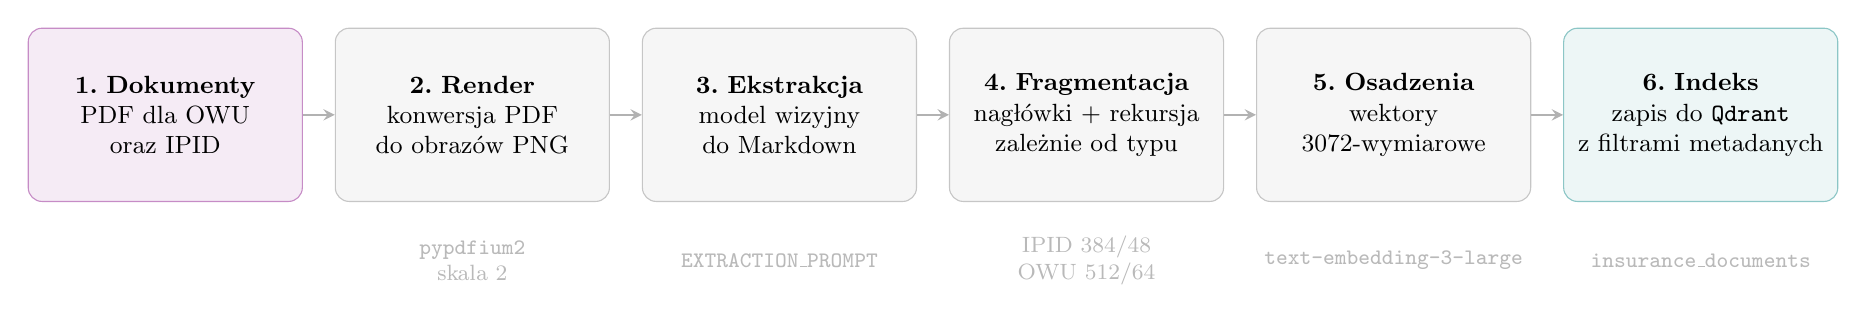
\begin{tikzpicture}[
        flowstep/.style={rectangle, draw, rounded corners=5pt,
          minimum width=3.4cm, minimum height=2.2cm,
          text width=3.2cm, align=center, font=\small,
        fill=gray!7, draw=gray!45, inner sep=4pt},
        arrow/.style={->, >=stealth, thick, draw=gray!60},
        lab/.style={font=\footnotesize, text=gray!55,
        align=center, text width=3.4cm}
      ]
      \node[flowstep, fill=violet!8, draw=violet!45] (pdf) at (0,    0)
      {\textbf{1.~Dokumenty}\\PDF dla OWU\\oraz IPID};
      \node[flowstep] (ocr)  at (3.9,  0)
      {\textbf{2.~Render}\\konwersja PDF\\do obrazów PNG};
      \node[flowstep] (md)   at (7.8,  0)
      {\textbf{3.~Ekstrakcja}\\model wizyjny\\do Markdown};
      \node[flowstep] (ch)   at (11.7, 0)
      {\textbf{4.~Fragmentacja}\\nagłówki + rekursja\\zależnie od typu};
      \node[flowstep] (emb)  at (15.6, 0)
      {\textbf{5.~Osadzenia}\\wektory\\3072-wymiarowe};
      \node[flowstep, fill=teal!7, draw=teal!45] (qd) at (19.5, 0)
      {\textbf{6.~Indeks}\\zapis do \texttt{Qdrant}\\z~filtrami metadanych};
      \foreach \a/\b in {pdf/ocr,ocr/md,md/ch,ch/emb,emb/qd}
      {\draw[arrow] (\a) -- (\b);}
      \node[lab] at (3.9,  -1.85) {\texttt{pypdfium2}\\skala 2};
      \node[lab] at (7.8,  -1.85) {\texttt{EXTRACTION\_PROMPT}};
      \node[lab] at (11.7, -1.85) {IPID 384/48\\OWU 512/64};
      \node[lab] at (15.6, -1.85) {\texttt{text-embedding-3-large}};
      \node[lab] at (19.5, -1.85) {\texttt{insurance\_documents}};
    \end{tikzpicture}
  \end{adjustbox}
  \zrodlo{opracowanie własne}
\end{figure}

\subsection{Ekstrakcja}\label{subsec:ekstrakcja}

Ekstrakcję realizuje klasa \texttt{Extractor} (\texttt{sources/extractor.py}).
Biblioteka \texttt{pypdfium2} renderuje obraz strony (skala 2), który -- po
zakodowaniu jako Base64 PNG -- trafia do modelu wizyjnego wraz z~promptem.
Kontekst międzystronicowy pozwala dołączyć 1024 znaki z~poprzedniej strony, co
zachowuje ciągłość sekcji rozbitych między arkuszami. Wywołanie powtarzane jest
maksymalnie pięciokrotnie z~wykładniczym opóźnieniem. Wynik stanowi plik
Markdown zapisany w~ustalonej strukturze katalogów.

\subsection{Fragmentacja}\label{subsec:fragmentacja}

Fragmentację tekstu wykonuje klasa \texttt{Chuncker}. Dokument dzielony jest
według nagłówków (poziomy 1--3), a~odpowiednie metadane propagowane są do
poszczególnych fragmentów. Większe sekcje podlegają fragmentacji rekurencyjnej
z~wykorzystaniem parametrów właściwych dla danego typu dokumentu
(tabela~\ref{tab:parametry-fragmentacji}).

\begin{table}[H]
  \caption{Parametry fragmentacji}\label{tab:parametry-fragmentacji}
  \centering
  \small
  \begin{tabular}{@{} l c c c @{}}
    \toprule
    \textbf{Typ dokumentu}
    & \textbf{Rozmiar fragmentu}
    & \textbf{Nakładanie}
    & \textbf{Minimum}                     \\
    \midrule
    IPID & 384                        & 48 & 48 \\
    OWU  & 512                        & 64 & 64 \\
    \bottomrule
  \end{tabular}
  \zrodlo{opracowanie własne}
\end{table}

Rozmiar fragmentów dla dokumentów IPID zredukowano ze względu na zwięzłość
formularzy, natomiast dla dokumentów OWU wartości zwiększono w~celu zachowania
kontekstu długich klauzul. Fragmentom przypisywany jest deterministyczny
identyfikator UUIDv5 (na bazie nazwy pliku, nagłówków i~treści).

\subsection{Indeksowanie}\label{subsec:indeksowanie}

Tworzenie indeksu realizuje klasa \texttt{VectorStore}
(\texttt{sources/vectorstore.py}). Inicjalizuje ona kolekcję
\texttt{insurance\_documents} z~miarą cosinusową, indeksem HNSW oraz indeksami
pól (payload). Przed wektoryzacją do treści fragmentu doklejane są metadane:
firma, produkt, kategoria, typ i~ścieżka nagłówków. Zabieg ten poprawia
dopasowanie wektorowe dla pytań uwzględniających ubezpieczyciela. Zapis w~bazie
\texttt{Qdrant} przebiega partiami. Pola strukturalne indeksowane są jako
\textit{keyword}, co gwarantuje stały czas działania filtrów metadanych.

\section{Infrastruktura ewaluacyjna}\label{sec:infrastruktura-ewaluacyjna}

Warstwę ewaluacyjną podzielono na trzy moduły. Komponent \texttt{Runner}
uruchamia architektury i~zapisuje odpowiedzi. \texttt{Evaluator} oblicza
metryki, korzystając z~usługi \texttt{Phoenix}. \texttt{Observer} inicjalizuje
śledzenie \texttt{OpenTelemetry} i~rejestruje przebiegi. Podział ten
uniezależnia generowanie odpowiedzi od oceny (architektury nie uzyskują
sprzężenia zwrotnego z~ewaluacji).

\subsection{Uruchamianie architektur}\label{subsec:uruchamianie-architektur}

Komponent \texttt{Runner} wczytuje pliki CSV z~pytaniami i~generuje iloczyn
kartezjański par pytanie--architektura (540 przebiegów dla 90 pytań). Wykonanie
zrównoleglono w~puli wątków, wykorzystując \texttt{graph.ainvoke}. Wyniki
logowane są w~sposób ciągły do plików JSONL i~CSV, co zapobiega utracie danych.
Pojedynczy rekord zawiera pytanie, wariant architektury, odpowiedź, metryki
wywołań, koszty oraz pełne metadane wykonania.

\subsection{Ocena odpowiedzi}\label{subsec:ocena-odpowiedzi}

Komponent \texttt{Evaluator} implementuje bibliotekę \texttt{phoenix.evals}.
Normalizuje wyniki i~wykonuje weryfikację pod kątem: wierności
(\textit{faithfulness}), zwięzłości (\textit{conciseness}) oraz poprawności
(\textit{correctness}). Trafność dokumentów (\textit{document relevance})
oceniana jest rozdzielnie (dla cytowanych fragmentów), co izoluje analizę
wyszukiwania od syntezy. Klasyfikatory poprawności i~zwięzłości wykorzystują
pięciostopniowe skale rzutowane na wartości numeryczne.

\subsection{Śledzenie przebiegów}\label{subsec:sledzenie-przebiegow}

Komponent \texttt{Observer} konfiguruje usługę \texttt{Phoenix}
(\texttt{auto\_instrument=True}), co zapewnia automatyczne śledzenie wywołań
bibliotek \texttt{LangChain} i~\texttt{OpenAI}. Ponadto zdefiniowano własne
zakresy monitorowania dla przebiegów architektur i~obliczeń metryk.

Tabela~\ref{tab:artefakty-ewaluacji} zestawia artefakty wyjściowe fazy
ewaluacji.

\begin{table}[H]
  \caption{Artefakty ewaluacji}\label{tab:artefakty-ewaluacji}
  \centering
  \small
  \begin{tabularx}{\textwidth}{@{} l L @{}}
    \toprule
    \textbf{Plik}
    & \textbf{Zawartość}                                    \\
    \midrule
    \texttt{runner\_results\_*.jsonl}
    & Strumieniowy zapis pełnych rekordów uruchomień        \\
    \texttt{runner\_results\_*.csv}
    & Spłaszczona tabela wyników wykonawczych               \\
    \texttt{runner\_results\_*.json}
    & Pełny zapis wyników po zakończeniu biegu              \\
    \texttt{runner\_summary\_*.csv}
    & Zbiorcze metryki operacyjne według architektury       \\
    \texttt{overall\_answer\_metrics\_*.csv}
    & Metryki odpowiedzi na poziomie pojedynczego przebiegu \\
    \texttt{overall\_document\_relevance\_*.csv}
    & Ocena trafności cytowanych fragmentów                 \\
    \texttt{overall\_summary\_*.csv}
    & Zbiorcze podsumowanie ewaluacji \texttt{Phoenix}      \\
    \bottomrule
  \end{tabularx}
  \zrodlo{opracowanie własne}
\end{table}

\section{Wybrane zagadnienia inżynieryjne}\label{sec:wybrane-zagadnienia-inzynieryjne}

\subsection{Zarządzanie rozmiarem okna kontekstowego}\label{subsec:kontrola-rozrostu-kontekstu}

W~systemach RAG nadmierny rozrost kontekstu stanowi istotne ograniczenie
techniczne. Moduł rerankera przycina fragmenty do 1000 znaków i~dzieli dane na
partie (limit 12000 tokenów). Selektor dowodów ogranicza kontekst syntezy do
\texttt{evidence\_top\_k} fragmentów. W~architekturze ReAct zamiast pełnej
treści dokumentów logowane są krótkie podsumowania działań narzędzi, co
uniezależnia rozmiar historii iteracji od liczby pobranych fragmentów.

\subsection{Agregacja metadanych wykonania}\label{subsec:spojnosc-metadanych-wykonania}

Metadane wykonania są agregowane przez funkcję
\texttt{merge\_tracking\_metadata}. Sumuje ona liczniki narzędzi, tokenów
i~kosztów przy jednoczesnym zachowaniu lokalnych zmiennych sterujących.
Mechanizm ten znajduje zastosowanie w~architekturze hierarchicznej oraz
w~funkcji \texttt{retrieve\_multi}, gdzie pojedyncze narzędzie wywoływane jest
wielokrotnie w~ramach jednego węzła.

\subsection{Obsługa niepoprawnych wyjść modeli}\label{subsec:odpornosc-na-niepoprawne-wyjscia-modeli}

Komponenty zależne od formatu JSON wyposażono w~ścieżki awaryjne. Parser zwraca
metadane neutralne, rewriter powiela zapytanie bazowe, planer stosuje wariant
deterministyczny, a~dekompozytor nie dzieli pytania. Architektura ReAct loguje
nierozpoznaną akcję jako obserwację. Błędy są rejestrowane, jednak system
gwarantuje zwrócenie kontrolowanego wyniku końcowego.

\subsection{Strategia wielojęzycznych promptów}\label{subsec:dwujezyczny-charakter-promptow}

Instrukcje systemowe sformułowano w~języku angielskim (z~uwagi na zwięzłość
i~zgodność z~formatami danych), natomiast pytania, dokumenty i~odpowiedzi
pozostają polskojęzyczne. Prompty odpowiedziowe wymuszają generowanie tekstu
w~języku polskim oraz zakazują korzystania z~wiedzy zewnętrznej.

\subsection{Stabilność identyfikatorów fragmentów}\label{subsec:idempotencja-indeksowania}

Identyfikatory fragmentów generowane są deterministycznie (algorytm UUIDv5) na
podstawie metadanych i~treści. Gwarantuje to identyczność kluczy w~bazie
\texttt{Qdrant} przy kolejnych uruchomieniach potoku dla niezmienionego
korpusu, co pozwala na przyrostową aktualizację i~porównywanie wyników.

\subsection{Izolacja warstwy ewaluacyjnej}\label{subsec:oddzielenie-ewaluacji-od-wykonania}

Ewaluator operuje wyłącznie na utrwalonych artefaktach. Architektury nie
modyfikują odpowiedzi na podstawie wyników z~\texttt{Phoenix}. Separacja ta
zapewnia odtwarzalność procesu: surowe pliki wynikowe mogą być poddawane
ponownej ocenie (z~użyciem innych ewaluatorów lub rubryk) bez konieczności
powtarzania przebiegów.
\chapter{Eksperyment i wyniki}\label{chap:eksperyment-i-wyniki}

Rozdział dokumentuje przebieg eksperymentu porównawczego oraz surowe wyniki
liczbowe. Ramy metodyczne i~kryteria oceny opisano w~\cref{chap:metodologia},
a~szczegóły implementacji -- w~\cref{chap:implementacja}. Niniejszy rozdział
ogranicza się do prezentacji danych i~wyników -- interpretację i~wnioski
omówiono w~rozdziale następnym.

\section{Przebieg wykonania}\label{sec:przebieg-wykonania}

Eksperyment zrealizowano w~ramach jednego uruchomienia obejmującego pełną
macierz \(90 \times 6 = 540\) par pytanie--architektura. Poniższe podsekcje
dokumentują czas trwania, kompletność wyników oraz zestaw wygenerowanych
artefaktów.

\subsection{Czas trwania}\label{subsec:czas-trwania}

Uruchomienie przeprowadzono 13~marca 2026~r. pod identyfikatorem
\texttt{20260313\_200511}. Komponent wykonawczy przekazał 540~par do puli
32~wątków roboczych; ostatni rekord zapisano o~\texttt{21:52~UTC}, co odpowiada
rzeczywistemu czasowi wykonania \mbox{1~h~47~min}. Łączny czas sekwencyjny --
rozumiany jako suma opóźnień wszystkich uruchomień -- wynosi \mbox{62\,698~s}
(\(\approx\)17{,}4~h). Faza ewaluacji jakościowej w~systemie \texttt{Phoenix}
zakończyła się o~\texttt{22:55~UTC}.

Tabela~\ref{tab:czas-wykonania} przedstawia rozkład czasu sekwencyjnego według
architektur wraz z~udziałem procentowym oraz średnim czasem pojedynczego
uruchomienia (z~odchyleniem standardowym). Architektura ReAct wykazała
największy udział w~łącznym czasie sekwencyjnym (26,1\%), natomiast
planer--wykonawca -- najmniejszy (12,1\%). Stanowi to interesujący paradoks
wydajnościowy: mimo dodatkowego narzutu czasowego na generowanie planu,
agent ten okazał się najszybszy w~ogólnej egzekucji (średnio 84{,}3~s),
wyprzedzając pod tym względem nawet najprostszą architekturę deterministyczną
(93{,}0~s). Wynika to z~faktu, że trafnie ułożony plan pozwolił na redukcję
liczby zbędnych wywołań narzędzi i~kosztownych operacji pobierania danych.

\begin{table}[H]
  \caption{Czas wykonania według architektury}\label{tab:czas-wykonania}
  \centering
  \small
  \renewcommand{\arraystretch}{1.3}
  \begin{tabular}{@{} l r r r r @{}}
    \toprule
    \textbf{Architektura}
    & \textbf{Uruchomienia}
    & \textbf{Suma opóźnień [s]}
    & \textbf{Udział [\%]}
    & \textbf{Średnia \(\pm\) odchylenie [s]}                                                                          \\
    \midrule
    Deterministyczna    & 90                                      & 8\,372           & 13{,}4           & 93{,}0 (\(\pm\) 17{,}5)          \\
    Planer--wykonawca   & 90                                      & 7\,583           & 12{,}1           & \textbf{84{,}3 (\(\pm\) 17{,}1)} \\
    Router--specjalista & 90                                      & 8\,902           & 14{,}2           & 98{,}9 (\(\pm\) 18{,}3)          \\
    Tablicowa           & 90                                      & 8\,229           & 13{,}1           & 91{,}4 (\(\pm\) 19{,}5)          \\
    Hierarchiczna       & 90                                      & 13\,239          & 21{,}1           & 147{,}1 (\(\pm\) 68{,}2)         \\
    ReAct               & 90                                      & \textbf{16\,374} & \textbf{26{,}1}  & 181{,}9 (\(\pm\) 44{,}9)         \\
    \midrule
    \textbf{Łącznie}    & \textbf{540}                            & \textbf{62\,698} & \textbf{100{,}0} & --                               \\
    \bottomrule
  \end{tabular}
  \zrodlo{opracowanie własne}
\end{table}

\subsection{Kompletność i~błędy wykonania}\label{subsec:kompletnosc-i-bledy}

Spośród 540~uruchomień 539 zakończyło się pomyślnie. Jedyny błąd odnotowano
w~architekturze hierarchicznej dla pytania dotyczącego zakresu autocasco na
terytorium Białorusi. Bezpośrednią przyczyną był wyjątek
\texttt{openai.BadRequestError~400} zwrócony przez interfejs \texttt{OpenAI
API}: węzeł dekompozytora wygenerował podpytanie w~mieszanym formacie
polsko-angielskim, co uniemożliwiło poprawną serializację odpowiedzi. Wyjątek
przechwycono i~zapisano jako rekord z~flagą błędu; zgodnie z~przyjętą procedurą
nie ponowiono wykonania zadania. Wskaźnik błędów wynosi \(1/540 \approx
0{,}19\%\) dla całego eksperymentu i~\(1{,}11\%\) dla architektury
hierarchicznej.

Żadne uruchomienie nie przekroczyło limitu czasowego 120~s. Nie odnotowano również
osiągnięcia limitu iteracji w~architekturach iteracyjnych; maksymalna liczba iteracji
architektury ReAct wyniosła~11 (przy progu równym 15).

\subsection{Artefakty wynikowe}\label{subsec:artefakty-wynikowe}

Wyniki uruchomienia zapisano w~katalogu \texttt{code/data/evaluation/results/}.
Tabela~\ref{tab:artefakty-wynikowe} zestawia pliki wyjściowe z~ich rozmiarami
i~zawartością; gwiazdka zastępuje pełny identyfikator uruchomienia
\texttt{20260313\_200511}. Największy rozmiar ma plik \texttt{.csv} z~surowymi
wynikami, natomiast plik zbiorczego podsumowania zajmuje poniżej 1~KB.

\begin{table}[H]
  \caption{Pliki wynikowe eksperymentu}\label{tab:artefakty-wynikowe}
  \centering
  \small
  \renewcommand{\arraystretch}{1.3}
  \begin{tabularx}{\textwidth}{@{} l r L @{}}
    \toprule
    \textbf{Plik}
    & \textbf{Rozmiar}
    & \textbf{Zawartość}                                     \\
    \midrule
    \texttt{runner\_results\_*.jsonl}
    & 16\,006~KB
    & 540~rekordów surowych w~formacie strumieniowym         \\
    \texttt{runner\_results\_*.csv}
    & 17\,131~KB
    & spłaszczona tabela 540~wierszy i~32~kolumn             \\
    \texttt{runner\_summary\_*.csv}
    & 2~KB
    & wartości zagregowane według architektury               \\
    \texttt{overall\_answer\_metrics\_*.csv}
    & 1\,988~KB
    & 539~ocen jakości odpowiedzi z~systemu \texttt{Phoenix} \\
    \texttt{overall\_document\_relevance\_*.csv}
    & 2\,216~KB
    & 1\,786~ocen trafności pojedynczych cytowań             \\
    \texttt{overall\_summary\_*.csv}
    & \({<}\)1~KB
    & zbiorcze miary jakości według architektury             \\
    \bottomrule
  \end{tabularx}
  \zrodlo{opracowanie własne}
\end{table}

\section{Wyniki operacyjne}\label{sec:wyniki-operacyjne}

W sekcji zestawiono średnie wartości miar opisujących zasobochłonność
uruchomień: zużycie tokenów i~koszt, liczbę wywołań narzędzi i~iteracji oraz
liczbę pobranych fragmentów i~cytowań. Wszystkie wartości w~tabelach podano
w~formacie średnia \(\pm\) odchylenie standardowe; podstawę obliczeń stanowi
90~uruchomień danej architektury, z~wyjątkiem hierarchicznej (89~uruchomień).

\subsection{Zużycie tokenów i~koszt}\label{subsec:zuzycie-tokenow-i-koszt}

Tabela~\ref{tab:tokeny-i-koszt} podaje średnie zużycie tokenów wejściowych
i~wyjściowych oraz średni koszt pojedynczego uruchomienia, oszacowany na
podstawie cennika \texttt{OpenAI API} obowiązującego w~marcu 2026~r.
Architektury jednoagentowe wykazują niewielki rozrzut: średnie zużycie tokenów
wejściowych mieści się w~przedziale 2\,988--3\,219, a~odchylenie standardowe
nie przekracza 260~tokenów. Architektury iteracyjne wykazują znaczną zmienność
-- średnia hierarchicznej wynosi 450\,017~tokenów wejściowych przy odchyleniu
standardowym 1\,080\,756, a~architektury ReAct 391\,935 przy odchyleniu
419\,373. Wartości odchylenia standardowego tak drastycznie przekraczające średnią
wynikają z~silnie prawostronnie skośnego rozkładu zużycia tokenów: w~większości
uruchomień agenci zużywają stosunkowo niewielką liczbę tokenów, jednak pojedyncze
przebiegi, w~których agent ulega zapętleniu lub wielokrotnie ponawia błędne
wywołania, konsumują ekstremalnie duże zasoby, co diametralnie zawyża średnią
i~wariancję. Średni koszt uruchomienia wynosi od 0{,}00037~USD (architektura
tablicowa) do 0{,}04320~USD (ReAct).

\begin{table}[H]
  \caption{Tokeny i~koszt na uruchomienie}\label{tab:tokeny-i-koszt}
  \centering
  \small
  \renewcommand{\arraystretch}{1.3}
  \begin{tabular}{@{} l r r r @{}}
    \toprule
    \textbf{Architektura}
    & \textbf{Tokeny wejściowe}      & \textbf{Tokeny wyjściowe}   & \textbf{Koszt [USD]}                  \\
    \midrule
    Deterministyczna    & \textbf{2\,988 (\(\pm\) 230)}  & 528 (\(\pm\) 160)           & 0{,}00038 (\(\pm\) 0{,}00007)          \\
    Planer--wykonawca   & 3\,219 (\(\pm\) 260)           & 580 (\(\pm\) 159)           & 0{,}00040 (\(\pm\) 0{,}00007)          \\
    Router--specjalista & 3\,199 (\(\pm\) 246)           & 519 (\(\pm\) 151)           & 0{,}00039 (\(\pm\) 0{,}00007)          \\
    Tablicowa           & 3\,004 (\(\pm\) 215)           & \textbf{498 (\(\pm\) 144)}  & \textbf{0{,}00037 (\(\pm\) 0{,}00006)} \\
    Hierarchiczna       & 450\,017 (\(\pm\) 1\,080\,756) & 115\,761 (\(\pm\) 303\,962) & 0{,}07109 (\(\pm\) 0{,}18099)          \\
    ReAct               & 391\,935 (\(\pm\) 419\,373)    & 58\,548 (\(\pm\) 66\,709)   & 0{,}04320 (\(\pm\) 0{,}04758)          \\
    \bottomrule
  \end{tabular}
  \zrodlo{opracowanie własne}
\end{table}

\subsection{Wywołania narzędzi i~iteracje}\label{subsec:wywolania-i-iteracje}

Tabela~\ref{tab:wywolania-i-iteracje} podaje średnią liczbę wywołań narzędzi
i~iteracji na uruchomienie wraz z~odchyleniem standardowym. Pojęcie iteracji
zależy od topologii: dla planera--wykonawcy oznacza długość wygenerowanego
planu, dla tablicowej -- liczbę cykli dyspozytora, dla hierarchicznej -- liczbę
przetworzonych podpytań, dla ReAct -- liczbę zarejestrowanych obserwacji.
Architektury deterministyczna i~router--specjalista nie posługują się pojęciem
iteracji. Architektura hierarchiczna wykonuje średnio 1\,066 wywołań narzędzi
na uruchomienie przy odchyleniu 2\,568, a~architektura ReAct 295{,}7 przy
odchyleniu 294{,}1. Planer--wykonawca wykazuje najniższą liczbę wywołań
narzędzi przy najmniejszym odchyleniu (średnio 7{,}2 przy odchyleniu 0{,}8).

\begin{table}[H]
  \caption{Liczba wywołań narzędzi i~iteracji na uruchomienie}\label{tab:wywolania-i-iteracje}
  \centering
  \small
  \renewcommand{\arraystretch}{1.3}
  \begin{tabular}{@{} l r r @{}}
    \toprule
    \textbf{Architektura}
    & \textbf{Wywołania narzędzi}     & \textbf{Iteracje}              \\
    \midrule
    Deterministyczna    & 10{,}0 (\(\pm\) 0{,}0)          & --                             \\
    Planer--wykonawca   & \textbf{7{,}2 (\(\pm\) 0{,}8)}  & \textbf{4{,}2 (\(\pm\) 0{,}8)} \\
    Router--specjalista & 9{,}8 (\(\pm\) 0{,}6)           & --                             \\
    Tablicowa           & 10{,}0 (\(\pm\) 0{,}0)          & 8{,}0 (\(\pm\) 0{,}0)          \\
    Hierarchiczna       & 1\,066{,}0 (\(\pm\) 2\,568{,}0) & 10{,}6 (\(\pm\) 4{,}8)         \\
    ReAct               & 295{,}7 (\(\pm\) 294{,}1)       & 7{,}7 (\(\pm\) 1{,}4)          \\
    \bottomrule
  \end{tabular}
  \zrodlo{opracowanie własne}
\end{table}

\subsection{Fragmenty z~wyszukiwania i~cytowania}\label{subsec:fragmenty-i-cytowania}

Tabela~\ref{tab:fragmenty-i-cytowania} przedstawia średnie liczby fragmentów
pobranych z~bazy \texttt{Qdrant} oraz cytowań w~odpowiedzi końcowej wraz
z~odchyleniami standardowymi. Kolumna \textit{Suma} podaje łączną liczbę
fragmentów pobranych w~obrębie jednego uruchomienia -- w~architekturach
iteracyjnych obejmuje wszystkie wywołania pętli roboczej lub obserwacyjnej.
Średnia łączna liczba fragmentów dla architektury hierarchicznej wynosi 1\,772
przy odchyleniu 4\,300, a~dla ReAct 154{,}5 przy odchyleniu 131{,}1.
Architektury jednoagentowe pobierają 5 lub 15~fragmentów na uruchomienie przy
zerowym lub minimalnym odchyleniu standardowym. W~architekturze ReAct liczba
cytowań w~odpowiedzi końcowej jest niższa niż w~pozostałych wariantach (średnio
  w~przedziale 3{,}29--3{,}82.

  Szczególną anomalię odnotowano w~przypadku architektury planera--wykonawcy.
  Zgodnie z~tabelą~\ref{tab:fragmenty-i-cytowania}, po etapie oceny trafności
  w~stanie agenta pozostaje średnio zaledwie 0{,}31 fragmentu, co świadczy
  o~niezwykle rygorystycznym odrzucaniu pobranego kontekstu przez sędziego.
  Paradoksalnie, odpowiedź końcowa generowana przez tę architekturę posiada
  średnio aż 3{,}38 cytowania. Wskazuje to na iluzję filtrowania dowodów:
  moduł syntezy w~przypadku planera zignorował wyniki oceny trafności
  i~samodzielnie uwzględnił fragmenty (bądź wyhalucynował ich znaczniki),
  które na etapie oceny zostały z~kontekstu usunięte.

  \begin{table}[H]
    \caption{Liczba fragmentów i~cytowań}\label{tab:fragmenty-i-cytowania}
    \centering
    \small
    \renewcommand{\arraystretch}{1.3}
    \begin{tabular}{@{} l r r r r @{}}
      \toprule
      \textbf{Architektura}
      & \textbf{Na zapytanie}            & \textbf{Suma}                   & \textbf{Po ocenie trafności}    & \textbf{Cytowania}               \\
      \midrule
      Deterministyczna    & \textbf{4{,}28 (\(\pm\) 1{,}00)} & 15{,}0 (\(\pm\) 0{,}0)          & 4{,}28 (\(\pm\) 1{,}00)         & 3{,}72 (\(\pm\) 0{,}67)          \\
      Planer--wykonawca   & 4{,}98 (\(\pm\) 0{,}15)          & \textbf{5{,}0 (\(\pm\) 0{,}0)}  & \textbf{0{,}31 (\(\pm\) 1{,}17)} & 3{,}38 (\(\pm\) 0{,}77)          \\
      Router--specjalista & 4{,}33 (\(\pm\) 0{,}99)          & 14{,}4 (\(\pm\) 2{,}0)          & 4{,}33 (\(\pm\) 0{,}99)         & 3{,}67 (\(\pm\) 0{,}65)          \\
      Tablicowa           & 4{,}30 (\(\pm\) 0{,}90)          & 15{,}0 (\(\pm\) 0{,}0)          & 4{,}30 (\(\pm\) 0{,}90)         & \textbf{3{,}74 (\(\pm\) 0{,}53)} \\
      Hierarchiczna       & 4{,}70 (\(\pm\) 1{,}48)          & 1\,771{,}7 (\(\pm\) 4\,299{,}8) & 4{,}70 (\(\pm\) 1{,}48)         & 3{,}74 (\(\pm\) 0{,}71)          \\
      ReAct               & 4{,}39 (\(\pm\) 1{,}07)          & 154{,}5 (\(\pm\) 131{,}1)       & 4{,}22 (\(\pm\) 1{,}32)         & 1{,}59 (\(\pm\) 1{,}69)          \\
      \bottomrule
    \end{tabular}
    \zrodlo{opracowanie własne}
  \end{table}

  \section{Wyniki jakościowe}\label{sec:wyniki-jakosciowe}

  Poniższe podsekcje przedstawiają wartości czterech miar jakości w~rozbiciu na
  architekturę, poziom trudności pytania, kategorię produktową i~ubezpieczyciela.
  Liczebności podzbiorów wynoszą: 9~pytań bardzo prostych, 27~prostych,
  27~złożonych i~27~bardzo złożonych; 30~pytań na każdą kategorię produktową
  i~30~na każdego ubezpieczyciela. W~architekturze hierarchicznej poziom złożony
  obejmuje 26~pytań ze względu na pojedynczy błąd wykonania.

  \subsection{Wierność}\label{subsec:wyniki-wiernosc}

  Tabele~\ref{tab:wiernosc-trudnosc}--\ref{tab:wiernosc-ubezpieczyciel}
  przedstawiają średnią wierność odpowiedzi wraz z~odchyleniem standardowym
  w~rozbiciu na poziom trudności, kategorię produktową i~ubezpieczyciela.
  Najwyższą wartość łączną osiąga router--specjalista (0{,}811), najniższą ReAct
  (0{,}611). Dla wszystkich architektur wierność spada wraz ze wzrostem poziomu
  trudności pytania. W~rozbiciu według kategorii produktowej i~ubezpieczyciela
  rozpiętość wyników między architekturami pozostaje zbliżona do rozpiętości
  w~ujęciu łącznym, z~jednym silnym wyjątkiem. Architektura ReAct odnotowała
  katastrofalny spadek wierności w~kategorii ubezpieczeń mieszkaniowych,
  uzyskując zaledwie 0{,}433 (wobec 0{,}667 dla ubezpieczeń komunikacyjnych
  i~0{,}733 dla turystycznych). Wynik bliski losowości wskazuje na wybitną
  podatność pętli obserwacyjnej ReAct na dryf semantyczny w~kategoriach
  o~szerszym i~bardziej podatnym na wieloznaczność zakresie pojęciowym.

  \begin{table}[H]
    \caption{Wierność według poziomu trudności}\label{tab:wiernosc-trudnosc}
    \centering
    \footnotesize
    \renewcommand{\arraystretch}{1.3}
    \begin{tabular}{@{} l c c c c c @{}}
      \toprule
      \textbf{Architektura}
      & \textbf{B.~proste}
      & \textbf{Proste}
      & \textbf{Złożone}
      & \textbf{B.~złożone}
      & \textbf{Łącznie}                                                                                                                                                                  \\
      \midrule
      Deterministyczna    & \textbf{0{,}889 (\(\pm\) 0{,}105)} & \textbf{0{,}852 (\(\pm\) 0{,}068)} & 0{,}741 (\(\pm\) 0{,}084)          & 0{,}704 (\(\pm\) 0{,}088)          & 0{,}778 (\(\pm\) 0{,}044)          \\
      Planer--wykonawca   & 0{,}889 (\(\pm\) 0{,}105)          & 0{,}741 (\(\pm\) 0{,}084)          & \textbf{0{,}852 (\(\pm\) 0{,}068)} & 0{,}741 (\(\pm\) 0{,}084)          & 0{,}789 (\(\pm\) 0{,}043)          \\
      Router--specjalista & 0{,}889 (\(\pm\) 0{,}105)          & 0{,}852 (\(\pm\) 0{,}068)          & 0{,}741 (\(\pm\) 0{,}084)          & \textbf{0{,}815 (\(\pm\) 0{,}075)} & \textbf{0{,}811 (\(\pm\) 0{,}041)} \\
      Tablicowa           & 0{,}778 (\(\pm\) 0{,}139)          & 0{,}852 (\(\pm\) 0{,}068)          & 0{,}704 (\(\pm\) 0{,}088)          & 0{,}815 (\(\pm\) 0{,}075)          & 0{,}789 (\(\pm\) 0{,}043)          \\
      Hierarchiczna       & 0{,}556 (\(\pm\) 0{,}166)          & 0{,}815 (\(\pm\) 0{,}075)          & 0{,}731 (\(\pm\) 0{,}087)          & 0{,}593 (\(\pm\) 0{,}095)          & 0{,}697 (\(\pm\) 0{,}049)          \\
      ReAct               & 0{,}556 (\(\pm\) 0{,}166)          & 0{,}667 (\(\pm\) 0{,}091)          & 0{,}519 (\(\pm\) 0{,}096)          & 0{,}667 (\(\pm\) 0{,}091)          & 0{,}611 (\(\pm\) 0{,}051)          \\
      \bottomrule
    \end{tabular}
    \zrodlo{opracowanie własne}
  \end{table}

  \begin{table}[H]
    \caption{Wierność według kategorii produktowej}\label{tab:wiernosc-kategoria}
    \centering
    \small
    \renewcommand{\arraystretch}{1.3}
    \begin{tabular}{@{} l c c c c @{}}
      \toprule
      \textbf{Architektura}
      & \textbf{Auto}
      & \textbf{Mieszkanie}
      & \textbf{Podróż}
      & \textbf{Łącznie}                                                                                                                              \\
      \midrule
      Deterministyczna    & 0{,}800 (\(\pm\) 0{,}073)          & 0{,}800 (\(\pm\) 0{,}073)          & 0{,}733 (\(\pm\) 0{,}081)          & 0{,}778 (\(\pm\) 0{,}044)          \\
      Planer--wykonawca   & 0{,}800 (\(\pm\) 0{,}073)          & \textbf{0{,}833 (\(\pm\) 0{,}068)} & 0{,}733 (\(\pm\) 0{,}081)          & 0{,}789 (\(\pm\) 0{,}043)          \\
      Router--specjalista & 0{,}800 (\(\pm\) 0{,}073)          & 0{,}833 (\(\pm\) 0{,}068)          & \textbf{0{,}800 (\(\pm\) 0{,}073)} & \textbf{0{,}811 (\(\pm\) 0{,}041)} \\
      Tablicowa           & \textbf{0{,}833 (\(\pm\) 0{,}068)} & 0{,}800 (\(\pm\) 0{,}073)          & 0{,}733 (\(\pm\) 0{,}081)          & 0{,}789 (\(\pm\) 0{,}043)          \\
      Hierarchiczna       & 0{,}586 (\(\pm\) 0{,}091)          & 0{,}700 (\(\pm\) 0{,}084)          & 0{,}800 (\(\pm\) 0{,}073)          & 0{,}697 (\(\pm\) 0{,}049)          \\
      ReAct               & 0{,}667 (\(\pm\) 0{,}086)          & 0{,}433 (\(\pm\) 0{,}090)          & 0{,}733 (\(\pm\) 0{,}081)          & 0{,}611 (\(\pm\) 0{,}051)          \\
      \bottomrule
    \end{tabular}
    \zrodlo{opracowanie własne}
  \end{table}

  \begin{table}[H]
    \caption{Wierność według ubezpieczyciela}\label{tab:wiernosc-ubezpieczyciel}
    \centering
    \small
    \renewcommand{\arraystretch}{1.3}
    \begin{tabular}{@{} l c c c c @{}}
      \toprule
      \textbf{Architektura}
      & \textbf{Hestia}
      & \textbf{PZU}
      & \textbf{Warta}
      & \textbf{Łącznie}                                                                                                                              \\
      \midrule
      Deterministyczna    & 0{,}700 (\(\pm\) 0{,}084)          & 0{,}800 (\(\pm\) 0{,}073)          & 0{,}833 (\(\pm\) 0{,}068)          & 0{,}778 (\(\pm\) 0{,}044)          \\
      Planer--wykonawca   & 0{,}733 (\(\pm\) 0{,}081)          & 0{,}800 (\(\pm\) 0{,}073)          & 0{,}833 (\(\pm\) 0{,}068)          & 0{,}789 (\(\pm\) 0{,}043)          \\
      Router--specjalista & 0{,}733 (\(\pm\) 0{,}081)          & 0{,}800 (\(\pm\) 0{,}073)          & \textbf{0{,}900 (\(\pm\) 0{,}055)} & \textbf{0{,}811 (\(\pm\) 0{,}041)} \\
      Tablicowa           & \textbf{0{,}833 (\(\pm\) 0{,}068)} & 0{,}767 (\(\pm\) 0{,}077)          & 0{,}767 (\(\pm\) 0{,}077)          & 0{,}789 (\(\pm\) 0{,}043)          \\
      Hierarchiczna       & 0{,}552 (\(\pm\) 0{,}092)          & \textbf{0{,}833 (\(\pm\) 0{,}068)} & 0{,}700 (\(\pm\) 0{,}084)          & 0{,}697 (\(\pm\) 0{,}049)          \\
      ReAct               & 0{,}633 (\(\pm\) 0{,}088)          & 0{,}733 (\(\pm\) 0{,}081)          & 0{,}467 (\(\pm\) 0{,}091)          & 0{,}611 (\(\pm\) 0{,}051)          \\
      \bottomrule
    \end{tabular}
    \zrodlo{opracowanie własne}
  \end{table}

  \subsection{Poprawność}\label{subsec:wyniki-poprawnosc}

  Tabele~\ref{tab:poprawnosc-trudnosc}--\ref{tab:poprawnosc-ubezpieczyciel}
  przedstawiają średnią poprawność odpowiedzi wraz z~odchyleniem standardowym
  w~tym samym rozbiciu. Najwyższą wartość łączną odnotowano dla architektury
  deterministycznej (0{,}716), a~najniższą dla hierarchicznej (0{,}588).
  W~rozbiciu według poziomu trudności poprawność przyjmuje najwyższe wartości dla
  pytań prostych we wszystkich wariantach, natomiast w~przypadku pytań bardzo
  złożonych ulega obniżeniu. W~rozbiciu według kategorii produktowej architektura
  deterministyczna osiągnęła najwyższe wartości we wszystkich trzech grupach.
  W~rozbiciu według ubezpieczyciela nie zaobserwowano jednoznacznej tendencji
  w~wynikach poszczególnych architektur.

  \begin{table}[H]
    \caption{Poprawność według poziomu trudności}\label{tab:poprawnosc-trudnosc}
    \centering
    \footnotesize
    \renewcommand{\arraystretch}{1.3}
    \begin{tabular}{@{} l c c c c c @{}}
      \toprule
      \textbf{Architektura}
      & \textbf{B.~proste}
      & \textbf{Proste}
      & \textbf{Złożone}
      & \textbf{B.~złożone}
      & \textbf{Łącznie}                                                                                                                                                                  \\
      \midrule
      Deterministyczna    & \textbf{0{,}644 (\(\pm\) 0{,}132)} & \textbf{0{,}841 (\(\pm\) 0{,}055)} & \textbf{0{,}685 (\(\pm\) 0{,}077)} & \textbf{0{,}644 (\(\pm\) 0{,}067)} & \textbf{0{,}716 (\(\pm\) 0{,}038)} \\
      Planer--wykonawca   & 0{,}578 (\(\pm\) 0{,}114)          & 0{,}681 (\(\pm\) 0{,}070)          & 0{,}596 (\(\pm\) 0{,}084)          & 0{,}596 (\(\pm\) 0{,}077)          & 0{,}620 (\(\pm\) 0{,}042)          \\
      Router--specjalista & 0{,}611 (\(\pm\) 0{,}116)          & 0{,}830 (\(\pm\) 0{,}053)          & 0{,}633 (\(\pm\) 0{,}078)          & 0{,}544 (\(\pm\) 0{,}073)          & 0{,}663 (\(\pm\) 0{,}039)          \\
      Tablicowa           & 0{,}544 (\(\pm\) 0{,}136)          & 0{,}807 (\(\pm\) 0{,}058)          & 0{,}633 (\(\pm\) 0{,}079)          & 0{,}489 (\(\pm\) 0{,}076)          & 0{,}633 (\(\pm\) 0{,}042)          \\
      Hierarchiczna       & 0{,}567 (\(\pm\) 0{,}119)          & 0{,}678 (\(\pm\) 0{,}076)          & 0{,}608 (\(\pm\) 0{,}077)          & 0{,}485 (\(\pm\) 0{,}079)          & 0{,}588 (\(\pm\) 0{,}043)          \\
      ReAct               & 0{,}633 (\(\pm\) 0{,}105)          & 0{,}704 (\(\pm\) 0{,}077)          & 0{,}567 (\(\pm\) 0{,}081)          & 0{,}515 (\(\pm\) 0{,}082)          & 0{,}599 (\(\pm\) 0{,}044)          \\
      \bottomrule
    \end{tabular}
    \zrodlo{opracowanie własne}
  \end{table}

  \begin{table}[H]
    \caption{Poprawność według kategorii produktowej}\label{tab:poprawnosc-kategoria}
    \centering
    \small
    \renewcommand{\arraystretch}{1.3}
    \begin{tabular}{@{} l c c c c @{}}
      \toprule
      \textbf{Architektura}
      & \textbf{Auto}
      & \textbf{Mieszkanie}
      & \textbf{Podróż}
      & \textbf{Łącznie}                                                                                                                              \\
      \midrule
      Deterministyczna    & \textbf{0{,}700 (\(\pm\) 0{,}068)} & 0{,}683 (\(\pm\) 0{,}076)          & \textbf{0{,}763 (\(\pm\) 0{,}052)} & \textbf{0{,}716 (\(\pm\) 0{,}038)} \\
      Planer--wykonawca   & 0{,}547 (\(\pm\) 0{,}079)          & 0{,}660 (\(\pm\) 0{,}064)          & 0{,}653 (\(\pm\) 0{,}072)          & 0{,}620 (\(\pm\) 0{,}042)          \\
      Router--specjalista & 0{,}593 (\(\pm\) 0{,}071)          & \textbf{0{,}690 (\(\pm\) 0{,}070)} & 0{,}707 (\(\pm\) 0{,}062)          & 0{,}663 (\(\pm\) 0{,}039)          \\
      Tablicowa           & 0{,}667 (\(\pm\) 0{,}066)          & 0{,}603 (\(\pm\) 0{,}077)          & 0{,}630 (\(\pm\) 0{,}074)          & 0{,}633 (\(\pm\) 0{,}042)          \\
      Hierarchiczna       & 0{,}562 (\(\pm\) 0{,}077)          & 0{,}570 (\(\pm\) 0{,}071)          & 0{,}630 (\(\pm\) 0{,}074)          & 0{,}588 (\(\pm\) 0{,}043)          \\
      ReAct               & 0{,}630 (\(\pm\) 0{,}078)          & 0{,}463 (\(\pm\) 0{,}077)          & 0{,}703 (\(\pm\) 0{,}065)          & 0{,}599 (\(\pm\) 0{,}044)          \\
      \bottomrule
    \end{tabular}
    \zrodlo{opracowanie własne}
  \end{table}

  \begin{table}[H]
    \caption{Poprawność według ubezpieczyciela}\label{tab:poprawnosc-ubezpieczyciel}
    \centering
    \small
    \renewcommand{\arraystretch}{1.3}
    \begin{tabular}{@{} l c c c c @{}}
      \toprule
      \textbf{Architektura}
      & \textbf{Hestia}
      & \textbf{PZU}
      & \textbf{Warta}
      & \textbf{Łącznie}                                                                                                                              \\
      \midrule
      Deterministyczna    & 0{,}693 (\(\pm\) 0{,}072)          & \textbf{0{,}793 (\(\pm\) 0{,}057)} & \textbf{0{,}660 (\(\pm\) 0{,}066)} & \textbf{0{,}716 (\(\pm\) 0{,}038)} \\
      Planer--wykonawca   & 0{,}697 (\(\pm\) 0{,}069)          & 0{,}640 (\(\pm\) 0{,}066)          & 0{,}523 (\(\pm\) 0{,}078)          & 0{,}620 (\(\pm\) 0{,}042)          \\
      Router--specjalista & 0{,}673 (\(\pm\) 0{,}070)          & 0{,}750 (\(\pm\) 0{,}060)          & 0{,}567 (\(\pm\) 0{,}070)          & 0{,}663 (\(\pm\) 0{,}039)          \\
      Tablicowa           & 0{,}683 (\(\pm\) 0{,}076)          & 0{,}623 (\(\pm\) 0{,}073)          & 0{,}593 (\(\pm\) 0{,}068)          & 0{,}633 (\(\pm\) 0{,}042)          \\
      Hierarchiczna       & 0{,}603 (\(\pm\) 0{,}078)          & 0{,}707 (\(\pm\) 0{,}065)          & 0{,}453 (\(\pm\) 0{,}072)          & 0{,}588 (\(\pm\) 0{,}043)          \\
      ReAct               & \textbf{0{,}720 (\(\pm\) 0{,}072)} & 0{,}567 (\(\pm\) 0{,}080)          & 0{,}510 (\(\pm\) 0{,}070)          & 0{,}599 (\(\pm\) 0{,}044)          \\
      \bottomrule
    \end{tabular}
    \zrodlo{opracowanie własne}
  \end{table}

  Szczegółowa analiza wyników poprawności w~zestawieniu z~wynikami trafności
  dokumentów (tabela~\ref{tab:trafnosc-ubezpieczyciel}) uwidacznia interesujący
  paradoks. Trafność pobierania dla dokumentów ubezpieczyciela Hestia jest
  systematycznie wyższa (od 0{,}406 do 0{,}480) niż dla dokumentów PZU
  (od 0{,}270 do 0{,}342). Jednakże w~przypadku wiodących architektur to właśnie
  pytania dotyczące PZU osiągają najwyższą poprawność w~fazie syntezy (0{,}793
  w~architekturze deterministycznej), podczas gdy dla Hestii wartości te są
  niższe (0{,}693). Sugeruje to, że dokumenty Hestii charakteryzują się formą
  sprzyjającą wyszukiwaniu wektorowemu (być może lepszą strukturą pojęciową),
  lecz trudniejszą do interpretacji przez model LLM, podczas gdy dokumenty PZU,
  mimo trudniejszego pozycjonowania w~przestrzeni osadzeń, posiadają zapisy,
  z~których łatwiej wydedukować jednoznaczną i~poprawną odpowiedź.

  \subsection{Zwięzłość}\label{subsec:wyniki-zwiezlosc}

  Tabele~\ref{tab:zwiezlosc-trudnosc}--\ref{tab:zwiezlosc-ubezpieczyciel}
  przedstawiają średnią zwięzłość odpowiedzi wraz z~odchyleniem standardowym.
  Wartości są bardziej zbliżone do siebie pomiędzy architekturami niż w~przypadku
  wierności i~poprawności -- mieszczą się w~przedziale 0{,}631--0{,}682.
  Najwyższą wartość łączną odnotowano dla wariantu ReAct (0{,}682), a~najniższą
  dla architektury deterministycznej (0{,}631). W~rozbiciu według poziomu
  trudności wartości zwięzłości nie wykazują jednoznacznej tendencji. W~rozbiciu
  według kategorii i~ubezpieczyciela różnice między architekturami pozostają
  niewielkie.

  \begin{table}[H]
    \caption{Zwięzłość według poziomu trudności}\label{tab:zwiezlosc-trudnosc}
    \centering
    \footnotesize
    \renewcommand{\arraystretch}{1.3}
    \begin{tabular}{@{} l c c c c c @{}}
      \toprule
      \textbf{Architektura}
      & \textbf{B.~proste}
      & \textbf{Proste}
      & \textbf{Złożone}
      & \textbf{B.~złożone}
      & \textbf{Łącznie}                                                                                                                                                                  \\
      \midrule
      Deterministyczna    & 0{,}544 (\(\pm\) 0{,}050)          & 0{,}630 (\(\pm\) 0{,}033)          & 0{,}648 (\(\pm\) 0{,}039)          & 0{,}644 (\(\pm\) 0{,}033)          & 0{,}631 (\(\pm\) 0{,}019)          \\
      Planer--wykonawca   & 0{,}667 (\(\pm\) 0{,}050)          & 0{,}637 (\(\pm\) 0{,}039)          & 0{,}630 (\(\pm\) 0{,}037)          & 0{,}689 (\(\pm\) 0{,}038)          & 0{,}653 (\(\pm\) 0{,}021)          \\
      Router--specjalista & \textbf{0{,}700 (\(\pm\) 0{,}047)} & 0{,}659 (\(\pm\) 0{,}031)          & 0{,}674 (\(\pm\) 0{,}035)          & 0{,}581 (\(\pm\) 0{,}037)          & 0{,}644 (\(\pm\) 0{,}019)          \\
      Tablicowa           & 0{,}678 (\(\pm\) 0{,}060)          & 0{,}674 (\(\pm\) 0{,}035)          & 0{,}626 (\(\pm\) 0{,}039)          & 0{,}652 (\(\pm\) 0{,}039)          & 0{,}653 (\(\pm\) 0{,}021)          \\
      Hierarchiczna       & 0{,}700 (\(\pm\) 0{,}047)          & \textbf{0{,}700 (\(\pm\) 0{,}038)} & \textbf{0{,}700 (\(\pm\) 0{,}037)} & 0{,}622 (\(\pm\) 0{,}040)          & 0{,}676 (\(\pm\) 0{,}021)          \\
      ReAct               & 0{,}611 (\(\pm\) 0{,}060)          & 0{,}685 (\(\pm\) 0{,}035)          & 0{,}689 (\(\pm\) 0{,}034)          & \textbf{0{,}696 (\(\pm\) 0{,}041)} & \textbf{0{,}682 (\(\pm\) 0{,}020)} \\
      \bottomrule
    \end{tabular}
    \zrodlo{opracowanie własne}
  \end{table}

  \begin{table}[H]
    \caption{Zwięzłość według kategorii produktowej}\label{tab:zwiezlosc-kategoria}
    \centering
    \small
    \renewcommand{\arraystretch}{1.3}
    \begin{tabular}{@{} l c c c c @{}}
      \toprule
      \textbf{Architektura}
      & \textbf{Auto}
      & \textbf{Mieszkanie}
      & \textbf{Podróż}
      & \textbf{Łącznie}                                                                                                                              \\
      \midrule
      Deterministyczna    & 0{,}610 (\(\pm\) 0{,}035)          & 0{,}630 (\(\pm\) 0{,}034)          & 0{,}653 (\(\pm\) 0{,}029)          & 0{,}631 (\(\pm\) 0{,}019)          \\
      Planer--wykonawca   & 0{,}700 (\(\pm\) 0{,}038)          & 0{,}613 (\(\pm\) 0{,}032)          & 0{,}647 (\(\pm\) 0{,}035)          & 0{,}653 (\(\pm\) 0{,}021)          \\
      Router--specjalista & 0{,}617 (\(\pm\) 0{,}034)          & \textbf{0{,}673 (\(\pm\) 0{,}031)} & 0{,}643 (\(\pm\) 0{,}033)          & 0{,}644 (\(\pm\) 0{,}019)          \\
      Tablicowa           & 0{,}657 (\(\pm\) 0{,}035)          & 0{,}623 (\(\pm\) 0{,}037)          & 0{,}680 (\(\pm\) 0{,}034)          & 0{,}653 (\(\pm\) 0{,}021)          \\
      Hierarchiczna       & 0{,}679 (\(\pm\) 0{,}031)          & 0{,}640 (\(\pm\) 0{,}038)          & \textbf{0{,}710 (\(\pm\) 0{,}038)} & 0{,}676 (\(\pm\) 0{,}021)          \\
      ReAct               & \textbf{0{,}737 (\(\pm\) 0{,}031)} & 0{,}660 (\(\pm\) 0{,}039)          & 0{,}650 (\(\pm\) 0{,}033)          & \textbf{0{,}682 (\(\pm\) 0{,}020)} \\
      \bottomrule
    \end{tabular}
    \zrodlo{opracowanie własne}
  \end{table}

  \begin{table}[H]
    \caption{Zwięzłość według ubezpieczyciela}\label{tab:zwiezlosc-ubezpieczyciel}
    \centering
    \small
    \renewcommand{\arraystretch}{1.3}
    \begin{tabular}{@{} l c c c c @{}}
      \toprule
      \textbf{Architektura}
      & \textbf{Hestia}
      & \textbf{PZU}
      & \textbf{Warta}
      & \textbf{Łącznie}                                                                                                                              \\
      \midrule
      Deterministyczna    & 0{,}647 (\(\pm\) 0{,}031)          & 0{,}597 (\(\pm\) 0{,}033)          & 0{,}650 (\(\pm\) 0{,}035)          & 0{,}631 (\(\pm\) 0{,}019)          \\
      Planer--wykonawca   & 0{,}633 (\(\pm\) 0{,}033)          & 0{,}673 (\(\pm\) 0{,}039)          & 0{,}653 (\(\pm\) 0{,}035)          & 0{,}653 (\(\pm\) 0{,}021)          \\
      Router--specjalista & 0{,}660 (\(\pm\) 0{,}027)          & 0{,}640 (\(\pm\) 0{,}031)          & 0{,}633 (\(\pm\) 0{,}039)          & 0{,}644 (\(\pm\) 0{,}019)          \\
      Tablicowa           & \textbf{0{,}697 (\(\pm\) 0{,}035)} & 0{,}653 (\(\pm\) 0{,}036)          & 0{,}610 (\(\pm\) 0{,}034)          & 0{,}653 (\(\pm\) 0{,}021)          \\
      Hierarchiczna       & 0{,}690 (\(\pm\) 0{,}035)          & 0{,}670 (\(\pm\) 0{,}033)          & 0{,}670 (\(\pm\) 0{,}040)          & 0{,}676 (\(\pm\) 0{,}021)          \\
      ReAct               & 0{,}647 (\(\pm\) 0{,}031)          & \textbf{0{,}697 (\(\pm\) 0{,}040)} & \textbf{0{,}703 (\(\pm\) 0{,}033)} & \textbf{0{,}682 (\(\pm\) 0{,}020)} \\
      \bottomrule
    \end{tabular}
    \zrodlo{opracowanie własne}
  \end{table}

  \subsection{Trafność dokumentów}\label{subsec:wyniki-trafnosc}

  Trafność dokumentów oceniano na poziomie pojedynczego cytowania -- łącznie
  1\,786~par pytanie--fragment.
  Tabele~\ref{tab:trafnosc-trudnosc}--\ref{tab:trafnosc-ubezpieczyciel} podają
  średnie arytmetyczne ocen binarnych wraz z~odchyleniem standardowym w~obrębie
  odpowiednich podzbiorów. Zaobserwowane wartości trafności są niższe niż
  w~przypadku pozostałych miar jakościowych i~mieszczą się w~przedziale
  0{,}332--0{,}364 dla wyników łącznych. Architektura deterministyczna i~ReAct
  osiągnęły tę samą najwyższą wartość (0{,}364), a~tablicowa najniższą (0{,}332).
  We wszystkich architekturach trafność przyjmuje wyższe wartości dla pytań
  bardzo prostych i~maleje wraz ze wzrostem poziomu trudności. W~rozbiciu według
  ubezpieczyciela najwyższe wartości we wszystkich architekturach odnotowano
  w~grupie \texttt{Hestia}, a~najniższe -- w~grupie \texttt{Warta}.

  \begin{table}[H]
    \caption{Trafność dokumentów według poziomu trudności}\label{tab:trafnosc-trudnosc}
    \centering
    \footnotesize
    \renewcommand{\arraystretch}{1.3}
    \begin{tabular}{@{} l c c c c c @{}}
      \toprule
      \textbf{Architektura}
      & \textbf{B.~proste}
      & \textbf{Proste}
      & \textbf{Złożone}
      & \textbf{B.~złożone}
      & \textbf{Łącznie}                                                                                                                                                                  \\
      \midrule
      Deterministyczna    & \textbf{0{,}545 (\(\pm\) 0{,}087)} & \textbf{0{,}394 (\(\pm\) 0{,}048)} & 0{,}330 (\(\pm\) 0{,}046)          & 0{,}305 (\(\pm\) 0{,}047)          & \textbf{0{,}364 (\(\pm\) 0{,}026)} \\
      Planer--wykonawca   & 0{,}500 (\(\pm\) 0{,}091)          & 0{,}323 (\(\pm\) 0{,}048)          & 0{,}359 (\(\pm\) 0{,}050)          & 0{,}315 (\(\pm\) 0{,}049)          & 0{,}349 (\(\pm\) 0{,}027)          \\
      Router--specjalista & 0{,}441 (\(\pm\) 0{,}085)          & 0{,}392 (\(\pm\) 0{,}050)          & 0{,}283 (\(\pm\) 0{,}045)          & \textbf{0{,}370 (\(\pm\) 0{,}048)} & 0{,}358 (\(\pm\) 0{,}026)          \\
      Tablicowa           & 0{,}500 (\(\pm\) 0{,}086)          & 0{,}307 (\(\pm\) 0{,}046)          & 0{,}337 (\(\pm\) 0{,}048)          & 0{,}298 (\(\pm\) 0{,}045)          & 0{,}332 (\(\pm\) 0{,}026)          \\
      Hierarchiczna       & 0{,}515 (\(\pm\) 0{,}087)          & 0{,}330 (\(\pm\) 0{,}046)          & 0{,}333 (\(\pm\) 0{,}047)          & 0{,}314 (\(\pm\) 0{,}046)          & 0{,}344 (\(\pm\) 0{,}026)          \\
      ReAct               & 0{,}500 (\(\pm\) 0{,}134)          & 0{,}370 (\(\pm\) 0{,}066)          & \textbf{0{,}419 (\(\pm\) 0{,}075)} & 0{,}219 (\(\pm\) 0{,}073)          & 0{,}364 (\(\pm\) 0{,}040)          \\
      \bottomrule
    \end{tabular}
    \zrodlo{opracowanie własne}
  \end{table}

  \begin{table}[H]
    \caption{Trafność dokumentów według kategorii produktowej}\label{tab:trafnosc-kategoria}
    \centering
    \small
    \renewcommand{\arraystretch}{1.3}
    \begin{tabular}{@{} l c c c c @{}}
      \toprule
      \textbf{Architektura}
      & \textbf{Auto}
      & \textbf{Mieszkanie}
      & \textbf{Podróż}
      & \textbf{Łącznie}                                                                                                                              \\
      \midrule
      Deterministyczna    & 0{,}315 (\(\pm\) 0{,}044)          & \textbf{0{,}386 (\(\pm\) 0{,}046)} & 0{,}391 (\(\pm\) 0{,}047)          & \textbf{0{,}364 (\(\pm\) 0{,}026)} \\
      Planer--wykonawca   & 0{,}323 (\(\pm\) 0{,}048)          & 0{,}383 (\(\pm\) 0{,}047)          & 0{,}337 (\(\pm\) 0{,}047)          & 0{,}349 (\(\pm\) 0{,}027)          \\
      Router--specjalista & \textbf{0{,}352 (\(\pm\) 0{,}046)} & 0{,}372 (\(\pm\) 0{,}045)          & 0{,}349 (\(\pm\) 0{,}046)          & 0{,}358 (\(\pm\) 0{,}026)          \\
      Tablicowa           & 0{,}315 (\(\pm\) 0{,}044)          & 0{,}342 (\(\pm\) 0{,}044)          & 0{,}339 (\(\pm\) 0{,}045)          & 0{,}332 (\(\pm\) 0{,}026)          \\
      Hierarchiczna       & 0{,}309 (\(\pm\) 0{,}044)          & 0{,}331 (\(\pm\) 0{,}043)          & \textbf{0{,}394 (\(\pm\) 0{,}047)} & 0{,}344 (\(\pm\) 0{,}026)          \\
      ReAct               & 0{,}318 (\(\pm\) 0{,}070)          & 0{,}372 (\(\pm\) 0{,}074)          & 0{,}393 (\(\pm\) 0{,}065)          & 0{,}364 (\(\pm\) 0{,}040)          \\
      \bottomrule
    \end{tabular}
    \zrodlo{opracowanie własne}
  \end{table}

  \begin{table}[H]
    \caption{Trafność dokumentów według ubezpieczyciela}\label{tab:trafnosc-ubezpieczyciel}
    \centering
    \small
    \renewcommand{\arraystretch}{1.3}
    \begin{tabular}{@{} l c c c c @{}}
      \toprule
      \textbf{Architektura}
      & \textbf{Hestia}
      & \textbf{PZU}
      & \textbf{Warta}
      & \textbf{Łącznie}                                                                                                                              \\
      \midrule
      Deterministyczna    & 0{,}460 (\(\pm\) 0{,}047)          & 0{,}336 (\(\pm\) 0{,}044)          & 0{,}294 (\(\pm\) 0{,}044)          & \textbf{0{,}364 (\(\pm\) 0{,}026)} \\
      Planer--wykonawca   & 0{,}406 (\(\pm\) 0{,}048)          & 0{,}333 (\(\pm\) 0{,}048)          & 0{,}304 (\(\pm\) 0{,}046)          & 0{,}349 (\(\pm\) 0{,}027)          \\
      Router--specjalista & 0{,}436 (\(\pm\) 0{,}047)          & 0{,}324 (\(\pm\) 0{,}046)          & \textbf{0{,}313 (\(\pm\) 0{,}043)} & 0{,}358 (\(\pm\) 0{,}026)          \\
      Tablicowa           & 0{,}425 (\(\pm\) 0{,}047)          & 0{,}270 (\(\pm\) 0{,}042)          & 0{,}301 (\(\pm\) 0{,}043)          & 0{,}332 (\(\pm\) 0{,}026)          \\
      Hierarchiczna       & 0{,}416 (\(\pm\) 0{,}046)          & \textbf{0{,}342 (\(\pm\) 0{,}045)} & 0{,}274 (\(\pm\) 0{,}042)          & 0{,}344 (\(\pm\) 0{,}026)          \\
      ReAct               & \textbf{0{,}480 (\(\pm\) 0{,}071)} & 0{,}302 (\(\pm\) 0{,}063)          & 0{,}300 (\(\pm\) 0{,}072)          & 0{,}364 (\(\pm\) 0{,}040)          \\
      \bottomrule
    \end{tabular}
    \zrodlo{opracowanie własne}
  \end{table}

  \section{Parametry konfiguracyjne eksperymentu}\label{sec:parametry-konfiguracyjne}

  Sekcja dokumentuje wartości parametrów sterujących przebiegiem uruchomienia.
  Pełną konfigurację zawierają moduły \texttt{sources/config/app.py}
  i~\texttt{sources/config/graph.py}; poniższe zestawienie obejmuje wyłącznie
  ustawienia użyte w~uruchomieniu \texttt{20260313\_200511}.

  \subsection{Parametry modeli językowych}\label{subsec:parametry-modeli}

  Wszystkie role pomocnicze -- parser, router, planer, kontroler ReAct, rewriter,
  dekompozytor i~ewaluator -- zrealizowano z~wykorzystaniem modelu
  \texttt{gpt-5}. Ten sam model zastosowano do syntezy odpowiedzi końcowej. Każdą
  rolę skonfigurowano z~temperaturą równą zero, limitem 120~s na pojedyncze
  wywołanie i~mechanizmem ponowień z~wykładniczym opóźnieniem od 1 do 60~s.
  Tabela~\ref{tab:parametry-modeli} zestawia pełną konfigurację.

  \begin{table}[H]
    \caption{Parametry modeli językowych}\label{tab:parametry-modeli}
    \centering
    \small
    \renewcommand{\arraystretch}{1.3}
    \begin{tabular}{@{} l l l @{}}
      \toprule
      \textbf{Parametr}
      & \textbf{Wartość}
      & \textbf{Rola}                                               \\
      \midrule
      \texttt{model\_name}
      & \texttt{gpt-5}   & model syntezy odpowiedzi                 \\
      \texttt{parser\_model\_name}
      & \texttt{gpt-5}   & parser pytań                             \\
      \texttt{router\_model\_name}
      & \texttt{gpt-5}   & router specjalisty                       \\
      \texttt{planner\_model\_name}
      & \texttt{gpt-5}   & planer kroków                            \\
      \texttt{controller\_model\_name}
      & \texttt{gpt-5}   & kontroler ReAct                          \\
      \texttt{rewrite\_model\_name}
      & \texttt{gpt-5}   & przepisywanie zapytań                    \\
      \texttt{decomposer\_model\_name}
      & \texttt{gpt-5}   & dekompozycja pytań                       \\
      \texttt{evaluation\_model\_name}
      & \texttt{gpt-5}   & sędzia jakości                           \\
      \texttt{temperature}
      & 0{,}0             & determinizm wyjścia                      \\
      \texttt{retry\_max\_attempts}
      & 5                & liczba ponowień                          \\
      \texttt{retry\_min\_wait}
      & 1{,}0~s          & minimalna pauza między ponowieniami      \\
      \texttt{retry\_max\_wait}
      & 60{,}0~s         & maksymalna pauza między ponowieniami     \\
      \texttt{llm\_request\_timeout}
      & 120{,}0~s        & limit pojedynczego wywołania             \\
      \texttt{max\_concurrent\_api\_calls}
      & 16               & limit równoległości wywołań \texttt{API} \\
      \bottomrule
    \end{tabular}
    \zrodlo{opracowanie własne na podstawie kodu źródłowego}
  \end{table}

  \subsection{Parametry wyszukiwania}\label{subsec:parametry-wyszukiwania}

  Wyszukiwanie wektorowe wykonano na kolekcji \texttt{insurance\_documents}
  w~bazie \texttt{Qdrant}, z~wykorzystaniem modelu osadzeń
  \texttt{text-embedding-3-large} o~wymiarze 3072. Etap rerankingu wyłączono we
  wszystkich architekturach; węzeł rerankera pozostał jednak obecny w~każdym
  grafie. Tabela~\ref{tab:parametry-wyszukiwania} prezentuje pełną konfigurację
  warstwy wyszukiwania wraz z~nominalnymi parametrami rerankera.

  \begin{table}[H]
    \caption{Parametry wyszukiwania}\label{tab:parametry-wyszukiwania}
    \centering
    \small
    \renewcommand{\arraystretch}{1.3}
    \begin{tabularx}{\textwidth}{@{} l l X @{}}
      \toprule
      \textbf{Parametr}
      & \textbf{Wartość}
      & \textbf{Opis}                                                              \\
      \midrule
      \texttt{embedding.model\_name}
      & \texttt{text-embedding-3-large} & model osadzeń                            \\
      \texttt{embedding.dimension}
      & 3072                            & wymiar wektora                           \\
      \texttt{qdrant.collection\_name}
      & \texttt{insurance\_documents}   & nazwa kolekcji                           \\
      \texttt{top\_k}
      & 5                               & liczba pobieranych fragmentów            \\
      \texttt{evidence\_top\_k}
      & 4                               & liczba dowodów przekazywanych do syntezy \\
      \texttt{reranking.enabled}
      & \texttt{False}                  & reranking wyłączony w~eksperymencie      \\
      \texttt{reranking.score\_threshold}
      & 0{,}3                            & próg odrzucenia fragmentu                \\
      \texttt{reranking.top\_k\_before}
      & 20                              & wejście do rerankera                     \\
      \texttt{reranking.top\_k\_after}
      & 5                               & wyjście z~rerankera                      \\
      \bottomrule
    \end{tabularx}
    \zrodlo{opracowanie własne na podstawie kodu źródłowego}
  \end{table}

  \subsection{Parametry fragmentacji}\label{subsec:parametry-fragmentacji}

  Dokumenty OWU i~IPID przetwarzano przy użyciu odrębnych profili fragmentacji.
  W~obu przypadkach zastosowano podział po nagłówkach Markdown poziomów 1--3,
  a~następnie rekurencyjną fragmentację większych sekcji. Parametry wyrażone
  w~liczbie znaków zestawiono w~tabeli~\ref{tab:parametry-fragmentacji};
  zastosowanie krótszych fragmentów dla IPID wynikało z~większej gęstości
  informacyjnej tego formatu.

  \begin{table}[H]
    \caption{Parametry fragmentacji dokumentów}\label{tab:parametry-fragmentacji}
    \centering
    \small
    \renewcommand{\arraystretch}{1.3}
    \begin{tabular}{@{} l c c l @{}}
      \toprule
      \textbf{Parametr}
      & \textbf{OWU}
      & \textbf{IPID}
      & \textbf{Opis}                                          \\
      \midrule
      \texttt{chunk\_size}      & 512           & 384 & docelowy rozmiar fragmentu       \\
      \texttt{chunk\_overlap}   & 64            & 48  & nakładanie sąsiednich fragmentów \\
      \texttt{min\_chunk\_size} & 64            & 48  & minimalny dopuszczalny rozmiar   \\
      \bottomrule
    \end{tabular}
    \zrodlo{opracowanie własne na podstawie kodu źródłowego}
  \end{table}

  \subsection{Parametry architektur}\label{subsec:parametry-architektur}

  Architektury iteracyjne wykorzystują jawne ograniczenia liczby kroków;
  architektura hierarchiczna ogranicza dekompozycję do trzech podpytań
  bezpośrednio w~kodzie węzła dekomponera. Architektury deterministyczna
  i~router--specjalista nie mają parametrów sterujących właściwych dla danej
  topologii. Tabela~\ref{tab:parametry-architektur} zestawia wartości dla
  wariantów, w~których takie parametry występują.

  \begin{table}[H]
    \caption{Parametry sterujące architektur}\label{tab:parametry-architektur}
    \centering
    \small
    \renewcommand{\arraystretch}{1.3}
    \begin{tabular}{@{} l l c l @{}}
      \toprule
      \textbf{Architektura}
      & \textbf{Parametr}
      & \textbf{Wartość}
      & \textbf{Znaczenie}                            \\
      \midrule
      ReAct
      & \texttt{max\_react\_iterations}          & 15
      & limit iteracji pętli obserwacyjnej            \\
      Tablicowa
      & \texttt{max\_blackboard\_iterations}     & 15
      & limit cykli dyspozytora                       \\
      Hierarchiczna
      & max. liczba podpytań                     & 3
      & przycięcie listy \texttt{sub\_questions}      \\
      \bottomrule
    \end{tabular}
    \zrodlo{opracowanie własne na podstawie kodu źródłowego}
  \end{table}

  \subsection{Parametry wykonania}\label{subsec:parametry-wykonania}

  Komponent wykonawczy pobierał parametry współbieżności
  z~\texttt{ConcurrencyConfig} i~inicjował pulę 32~wątków obsługujących pełną
  macierz par pytanie--architektura. Tabela~\ref{tab:parametry-wykonania}
  przedstawia liczebności i~ustawienia dla uruchomienia \texttt{20260313\_200511}.

  \begin{table}[H]
    \caption{Parametry wykonania eksperymentu}\label{tab:parametry-wykonania}
    \centering
    \small
    \renewcommand{\arraystretch}{1.3}
    \begin{tabular}{@{} l c l @{}}
      \toprule
      \textbf{Parametr}
      & \textbf{Wartość}
      & \textbf{Opis}                                            \\
      \midrule
      \texttt{max\_workers}    & 32               & rozmiar puli wątków roboczych         \\
      Liczba pytań testowych   & 90               & zestaw \texttt{pytania\_20251130.csv} \\
      Liczba architektur       & 6                & komplet \texttt{ALL\_PATTERNS}        \\
      Łączna liczba uruchomień & 540              & macierz \(90 \times 6\)               \\
      \bottomrule
    \end{tabular}
    \zrodlo{opracowanie własne na podstawie kodu źródłowego}
  \end{table}
\chapter{Wnioski i~zakończenie}\label{chap:wnioski-i-zakonczenie}

Rozdział podsumowuje pracę na podstawie wyników
z~\cref{chap:eksperyment-i-wyniki}. Kolejne sekcje obejmują analizę ilościową
czterech miar jakości i~zestawu miar operacyjnych, analizę jakościową typowych
wzorców niepowodzeń, rozstrzygnięcie głównego problemu badawczego, odpowiedzi
na pytania badawcze oraz ocenę realizacji celów badawczych sformułowanych
w~\cref{chap:wprowadzenie}, kierunki dalszych badań, rekomendacje dla praktyków
oraz podsumowanie pracy.

\section{Wnioski ilościowe}\label{sec:wnioski-ilosciowe}

Analiza wszystkich miar wskazuje na podział sześciu architektur na dwie grupy.
Pierwszą tworzą architektury: deterministyczna, planer--wykonawca,
router--specjalista i~tablicowa, których wyniki różnią się nieznacznie. Drugą
stanowią dwa warianty iteracyjne o~wysokim narzucie operacyjnym: hierarchiczna
i~ReAct, które osiągają niższe wyniki w~większości miar i~generują wyższe
koszty.

\subsection{Wierność}\label{subsec:wiernosc}

Wartości wierności wynoszą od 0{,}611 do 0{,}811. Cztery architektury
z~pierwszej grupy osiągają wyniki w~przedziale 0{,}778--0{,}811, podczas gdy
architektura hierarchiczna uzyskuje 0{,}697, a~ReAct 0{,}611
(tabela~\ref{tab:wiernosc-trudnosc}). Maksymalna różnica wynosi 0{,}200 punktu
i~wynika z~odstępstwa wariantów iteracyjnych od pierwszej grupy architektur.

\begin{wykres}[H]
  \caption{Wierność według architektury}\label{wykres:wiernosc-per-architektura}
  \centering
  \begin{adjustbox}{max width=0.82\textwidth}
    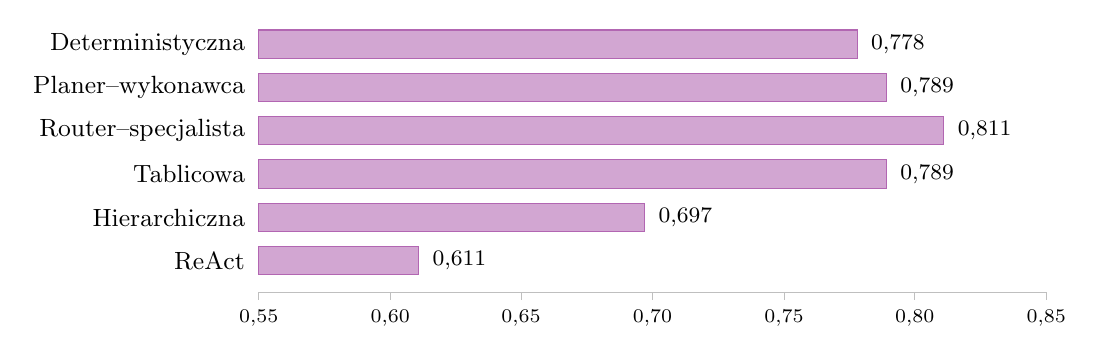
\begin{tikzpicture}[
        archlbl/.style={font=\small, anchor=east, inner sep=2pt},
        valuelbl/.style={font=\footnotesize, anchor=west, inner sep=2pt},
        ticklbl/.style={font=\scriptsize, anchor=north},
        baraxis/.style={draw=gray!50, line width=0.3pt}
      ]
      \def\bw{10}
      \def\bh{0.18}
      \foreach \name/\barlen/\lbl/\y in {%
        Deterministyczna/7.60/0{,}778/0,
        Planer--wykonawca/7.97/0{,}789/-0.55,
        Router--specjalista/8.70/0{,}811/-1.10,
        Tablicowa/7.97/0{,}789/-1.65,
        Hierarchiczna/4.90/0{,}697/-2.20,
        ReAct/2.03/0{,}611/-2.75%
      }{
        \node[archlbl] at (-0.1,\y) {\name};
        \fill[violet!35, draw=violet!60]
        (0,\y-\bh) rectangle (\barlen,\y+\bh);
        \node[valuelbl] at ({\barlen+0.1},\y) {\lbl};
      }
      \draw[baraxis] (0,-3.15) -- (\bw,-3.15);
      \foreach \v/\lbl in {
        0/0{,}55, 1.67/0{,}60, 3.33/0{,}65, 5/0{,}70,
      6.67/0{,}75, 8.33/0{,}80, 10/0{,}85} {
        \draw[baraxis] (\v,-3.15) -- (\v,-3.25);
        \node[ticklbl] at (\v,-3.25) {\lbl};
      }
    \end{tikzpicture}
  \end{adjustbox}
  \zrodlo{opracowanie własne}
\end{wykres}

Najwyższy wynik routera--specjalisty (0{,}811) wynika z~mechanizmu klasyfikacji
pytania do jednej z~ośmiu kategorii semantycznych przed pobraniem fragmentów.
Klasyfikator zawęża obszar wyszukiwania do fragmentów właściwych dla danego
typu pytania, ograniczając liczbę kontekstów semantycznie zbliżonych, lecz
produktowo nieadekwatnych. Różnicę tę zaobserwowano dla pytań bardzo złożonych
(0{,}815 wobec 0{,}704 architektury deterministycznej), natomiast nie występuje
ona dla pytań prostszych, dla których przestrzeń wyszukiwania jest jednoznaczna
bez trasowania.

Niższa wierność w~architekturze hierarchicznej (0{,}697) wynika z~dwóch
czynników. Pierwszym jest bezwarunkowe uruchomienie dekompozytora: pytania
jednoaspektowe są rozkładane na podpytania, co skutkuje wzrostem liczby
kontekstów dostarczanych do syntezy. Drugim jest węzeł scalający, który
uzupełnia odpowiedzi z~podpytań elementami z~wiedzy parametrycznej modelu
zamiast wyłącznie z~pobranych fragmentów.

Architektura ReAct uzyskuje najniższą wierność (0{,}611) z~powodu dryfu
kontrolera w~pętli myśl--działanie. Po kilku iteracjach przepisane zapytania
stopniowo poszerzają zakres tematyczny: zapytania o~konkretny produkt są
zastępowane zapytaniami ogólniejszymi, zwracającymi fragmenty z~innych
ubezpieczycieli i~innych produktów. Wygenerowane odpowiedzi są spójne lokalnie,
lecz odnoszą się do produktu innego niż przedmiot pytania.

Cztery architektury z~pierwszej grupy różnią się między sobą o~0{,}033 punktu.
Przy próbie 90~pytań różnica ta nie jest statystycznie istotna; jedyną parą
wykazującą istotną różnicę jest router--specjalista i~ReAct.

\subsection{Poprawność}\label{subsec:poprawnosc}

Najwyższą poprawność osiąga architektura deterministyczna (0{,}716). Drugą
pozycję zajmuje router--specjalista (0{,}663), natomiast architektura
hierarchiczna uzyskuje najniższy wynik: 0{,}588
(tabela~\ref{tab:poprawnosc-trudnosc}).

\begin{wykres}[H]
  \caption{Poprawność według architektury}\label{wykres:poprawnosc-per-architektura}
  \centering
  \begin{adjustbox}{max width=0.82\textwidth}
    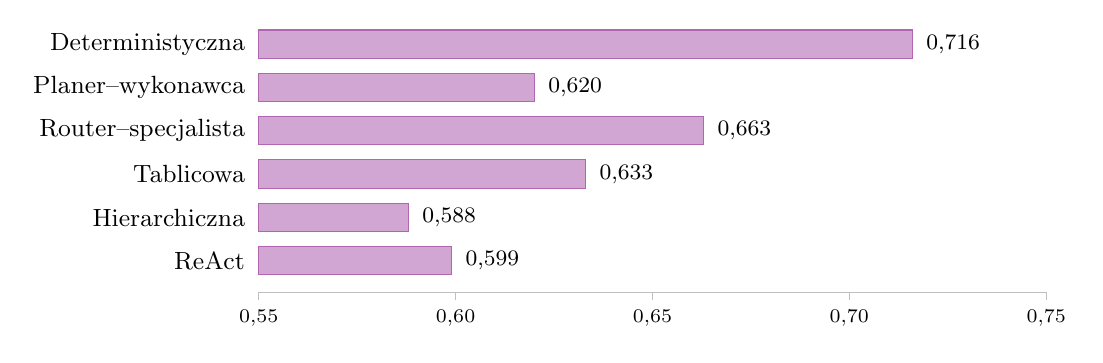
\begin{tikzpicture}[
        archlbl/.style={font=\small, anchor=east, inner sep=2pt},
        valuelbl/.style={font=\footnotesize, anchor=west, inner sep=2pt},
        ticklbl/.style={font=\scriptsize, anchor=north},
        baraxis/.style={draw=gray!50, line width=0.3pt}
      ]
      \def\bw{10}
      \def\bh{0.18}
      \foreach \name/\barlen/\lbl/\y in {%
        Deterministyczna/8.30/0{,}716/0,
        Planer--wykonawca/3.50/0{,}620/-0.55,
        Router--specjalista/5.65/0{,}663/-1.10,
        Tablicowa/4.15/0{,}633/-1.65,
        Hierarchiczna/1.90/0{,}588/-2.20,
        ReAct/2.45/0{,}599/-2.75%
      }{
        \node[archlbl] at (-0.1,\y) {\name};
        \fill[violet!35, draw=violet!60]
        (0,\y-\bh) rectangle (\barlen,\y+\bh);
        \node[valuelbl] at ({\barlen+0.1},\y) {\lbl};
      }
      \draw[baraxis] (0,-3.15) -- (\bw,-3.15);
      \foreach \v/\lbl in {
      0/0{,}55, 2.5/0{,}60, 5/0{,}65, 7.5/0{,}70, 10/0{,}75} {
        \draw[baraxis] (\v,-3.15) -- (\v,-3.25);
        \node[ticklbl] at (\v,-3.25) {\lbl};
      }
    \end{tikzpicture}
  \end{adjustbox}
  \zrodlo{opracowanie własne}
\end{wykres}

Wyższy wynik architektury deterministycznej jest następstwem braku węzłów
decyzyjnych: pojedyncza ścieżka wykonania nie wprowadza ryzyka błędnej
klasyfikacji, dekompozycji ani trasowania. Każdy taki węzeł w~pozostałych
architekturach jest potencjalnym źródłem rozbieżności z~odpowiedzią
referencyjną. W~przypadku routera--specjalisty część pytań kierowana jest do
podpotoku niezgodnego z~referencyjną klasyfikacją; wybrany podpotok pomija
klauzule istotne dla pytania, mimo że zwracane fragmenty są wewnętrznie spójne.

Rozbieżność między wiernością a~poprawnością wynika z~definicji obu miar.
Odpowiedź może być wierna wobec pobranych fragmentów, a~jednocześnie niezgodna
z~ odpowiedzią referencyjną, jeśli pobrane fragmenty opisują niekompletny stan
faktyczny. Router--specjalista osiąga wyższą wierność, lecz niższą poprawność
niż architektura deterministyczna: wąskie wyszukiwanie ogranicza ryzyko
halucynacji, lecz zwiększa ryzyko pominięcia kontekstu z~innej części
dokumentu.

W~obu wariantach iteracyjnych zaobserwowano spadek poprawności dla pytań bardzo
złożonych (hierarchiczna 0{,}485, ReAct 0{,}515). Przy tym poziomie trudności
pytanie wymaga zestawienia kilku klauzul z~różnych części dokumentu -- oba
kontrolery pobierają te fragmenty, lecz węzeł syntezy nie scala ich poprawnie
przy nadmiarze kontekstu.

\subsection{Zwięzłość}\label{subsec:zwiezlosc}

Wyniki w~zakresie zwięzłości wykazują najmniejszą wariancję. Wszystkie
architektury osiągają wartości w~przedziale 0{,}631--0{,}682, a~maksymalna
różnica wynosi 0{,}051 punktu (tabela~\ref{tab:zwiezlosc-trudnosc}). Wskazuje
to, że dominującym czynnikiem długości i~gęstości informacyjnej odpowiedzi jest
wspólny prompt syntezy, a~nie topologia sterowania.

\begin{wykres}[H]
  \caption{Zwięzłość według architektury}\label{wykres:zwiezlosc-per-architektura}
  \centering
  \begin{adjustbox}{max width=0.82\textwidth}
    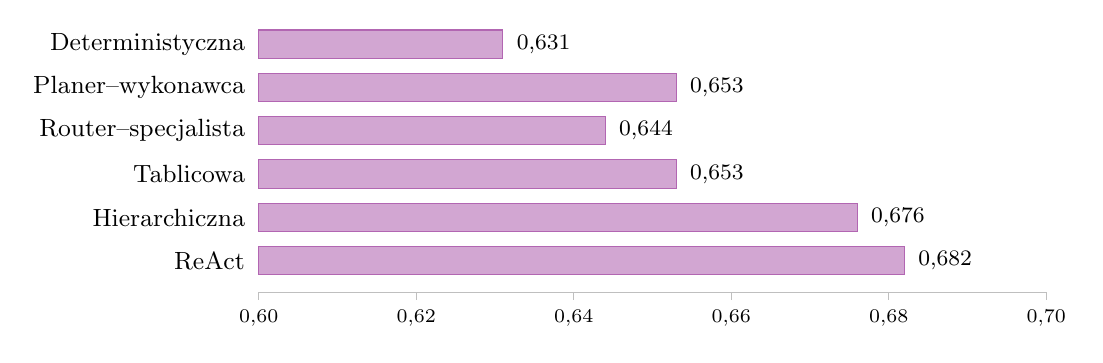
\begin{tikzpicture}[
        archlbl/.style={font=\small, anchor=east, inner sep=2pt},
        valuelbl/.style={font=\footnotesize, anchor=west, inner sep=2pt},
        ticklbl/.style={font=\scriptsize, anchor=north},
        baraxis/.style={draw=gray!50, line width=0.3pt}
      ]
      \def\bw{10}
      \def\bh{0.18}
      \foreach \name/\barlen/\lbl/\y in {%
        Deterministyczna/3.10/0{,}631/0,
        Planer--wykonawca/5.30/0{,}653/-0.55,
        Router--specjalista/4.40/0{,}644/-1.10,
        Tablicowa/5.30/0{,}653/-1.65,
        Hierarchiczna/7.60/0{,}676/-2.20,
        ReAct/8.20/0{,}682/-2.75%
      }{
        \node[archlbl] at (-0.1,\y) {\name};
        \fill[violet!35, draw=violet!60]
        (0,\y-\bh) rectangle (\barlen,\y+\bh);
        \node[valuelbl] at ({\barlen+0.1},\y) {\lbl};
      }
      \draw[baraxis] (0,-3.15) -- (\bw,-3.15);
      \foreach \v/\lbl in {
      0/0{,}60, 2/0{,}62, 4/0{,}64, 6/0{,}66, 8/0{,}68, 10/0{,}70} {
        \draw[baraxis] (\v,-3.15) -- (\v,-3.25);
        \node[ticklbl] at (\v,-3.25) {\lbl};
      }
    \end{tikzpicture}
  \end{adjustbox}
  \zrodlo{opracowanie własne}
\end{wykres}

Najwyższy wynik ReAct (0{,}682) wynika z~mechanizmu obserwacji: kontroler
filtruje fragmenty zwrócone przez wcześniejsze wywołania narzędzi i~przekazuje
do syntezy mniejszy zbiór dowodów (średnio 1{,}59~cytowania w~odpowiedzi
końcowej, tabela~\ref{tab:fragmenty-i-cytowania}). Najniższy wynik architektury
deterministycznej (0{,}631) wynika z~odwrotnego zjawiska: synteza otrzymuje
pełny zestaw 4{,}28~fragmentów po reranku i~uwzględnia każdy z~nich
w~odpowiedzi wraz z~cytowaniem.

Praktyczne znaczenie tej miary jest jednak ograniczone w~kontekście dokumentów
regulacyjnych. Zbyt zwięzła odpowiedź może pomijać warunek dodatkowy,
stanowiący integralną część prawidłowej odpowiedzi. Wzrost zwięzłości nie
powinien być traktowany jako poprawa jakości bez równoczesnej weryfikacji
poprawności i~kompletności.

\subsection{Trafność dokumentów}\label{subsec:trafnosc-dokumentow}

Wartości trafności dokumentów są niskie we~wszystkich architekturach --
wartości łączne wynoszą od 0{,}332 do 0{,}364
(tabela~\ref{tab:trafnosc-trudnosc}). Rozpiętość między architekturami wynosi
0{,}032 punktu, co wskazuje, że ograniczenie leży poza warstwą orkiestracji.

\begin{wykres}[H]
  \caption{Trafność dokumentów według architektury}\label{wykres:trafnosc-dokumentow-per-architektura}
  \centering
  \begin{adjustbox}{max width=0.82\textwidth}
    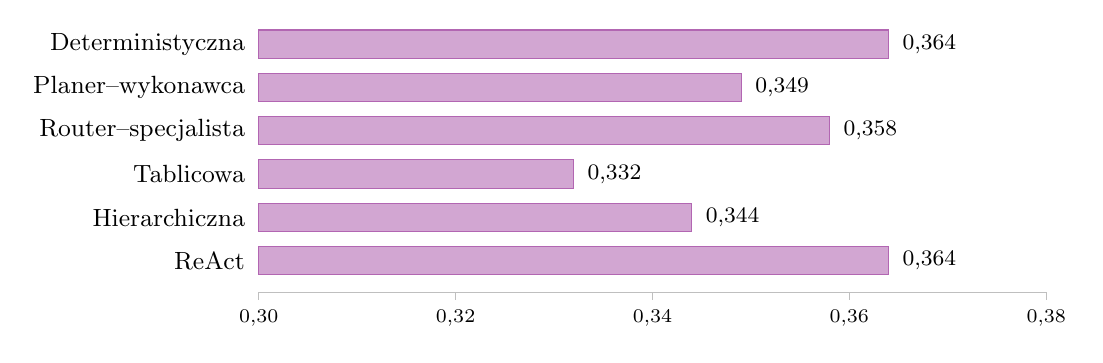
\begin{tikzpicture}[
        archlbl/.style={font=\small, anchor=east, inner sep=2pt},
        valuelbl/.style={font=\footnotesize, anchor=west, inner sep=2pt},
        ticklbl/.style={font=\scriptsize, anchor=north},
        baraxis/.style={draw=gray!50, line width=0.3pt}
      ]
      \def\bw{10}
      \def\bh{0.18}
      \foreach \name/\barlen/\lbl/\y in {%
        Deterministyczna/8.00/0{,}364/0,
        Planer--wykonawca/6.13/0{,}349/-0.55,
        Router--specjalista/7.25/0{,}358/-1.10,
        Tablicowa/4.00/0{,}332/-1.65,
        Hierarchiczna/5.50/0{,}344/-2.20,
        ReAct/8.00/0{,}364/-2.75%
      }{
        \node[archlbl] at (-0.1,\y) {\name};
        \fill[violet!35, draw=violet!60]
        (0,\y-\bh) rectangle (\barlen,\y+\bh);
        \node[valuelbl] at ({\barlen+0.1},\y) {\lbl};
      }
      \draw[baraxis] (0,-3.15) -- (\bw,-3.15);
      \foreach \v/\lbl in {
      0/0{,}30, 2.5/0{,}32, 5/0{,}34, 7.5/0{,}36, 10/0{,}38} {
        \draw[baraxis] (\v,-3.15) -- (\v,-3.25);
        \node[ticklbl] at (\v,-3.25) {\lbl};
      }
    \end{tikzpicture}
  \end{adjustbox}
  \zrodlo{opracowanie własne}
\end{wykres}

Główną przyczyną tego zjawiska we~wszystkich wariantach jest sposób
reprezentacji wektorowej dokumentów ubezpieczeniowych. Klauzule ochrony
i~klauzule wyłączeń zajmują w~przestrzeni osadzeń różne pozycje względem
typowego pytania. Pytania klientów są formułowane afirmatywnie (,,czy
ubezpieczenie obejmuje X?''), a~wyszukiwanie kosinusowe faworyzuje fragmenty
o~zbliżonej polaryzacji. Klauzule wyłączeń, formułowane przez negację, są
systematycznie przesuwane w~dół rankingu, mimo że niejednokrotnie zawierają
kluczową odpowiedź. Trafność wykazuje ponadto tendencję spadkową wraz
z~poziomem trudności pytania: z~zakresu 0{,}441--0{,}545 dla pytań bardzo
prostych do 0{,}219--0{,}370 dla bardzo złożonych.

Dodatkowo zaobserwowano swoisty paradoks pomiędzy trafnością pobierania a~końcową
poprawnością odpowiedzi w~zależności od dokumentów ubezpieczyciela.
Dokumenty Hestii osiągają systematycznie wyższą trafność wyszukiwania
(do 0{,}480) niż dokumenty PZU (ok.~0{,}33), co sugeruje strukturę silnie
sprzyjającą reprezentacji wektorowej. Z~kolei najwyższą poprawność końcowej
syntezy (np.~0{,}793 w~ariancie deterministycznym) wiodące architektury
odnotowują dla PZU, a~nie Hestii. Oznacza to, że wysoka trafność fragmentów
nie implikuje wprost sukcesu informacyjnego -- dokumenty trudniejsze do
wyszukania (PZU) okazały się dla modelu językowego językowo łatwiejsze do
poprawnej interpretacji i~złożenia ostatecznej odpowiedzi.

Drugim ograniczeniem jest oddzielenie sekcji definicyjnych od klauzul,
w~których definiowane terminy są używane. Pojęcia takie jak suma ubezpieczenia,
franszyza redukcyjna czy wartość rynkowa pojazdu są definiowane w~paragrafach
wstępnych i~używane w~odległych częściach dokumentu bez powtórzenia definicji.
Pojedyncze zapytanie pozwala zidentyfikować klauzulę użycia, lecz omija sekcję
definicji, co obniża trafność cytowania bez naruszenia wierności odpowiedzi.

\subsection{Koszty operacyjne}\label{subsec:koszty-operacyjne}

Wariancja kosztów operacyjnych między architekturami jest większa niż
w~przypadku jakiejkolwiek miary jakości. Średni koszt jednego uruchomienia
wynosi od 0{,}00037 do 0{,}00040~USD dla czterech architektur o~stałym lub
płytko sterowanym przebiegu i~wzrasta do 0{,}04320~USD dla ReAct oraz
0{,}07109~USD dla architektury hierarchicznej
(tabela~\ref{tab:tokeny-i-koszt}).

\begin{wykres}[H]
  \caption{Koszt na uruchomienie w~skali logarytmicznej}\label{wykres:koszt-per-uruchomienie}
  \centering
  \begin{adjustbox}{max width=0.82\textwidth}
    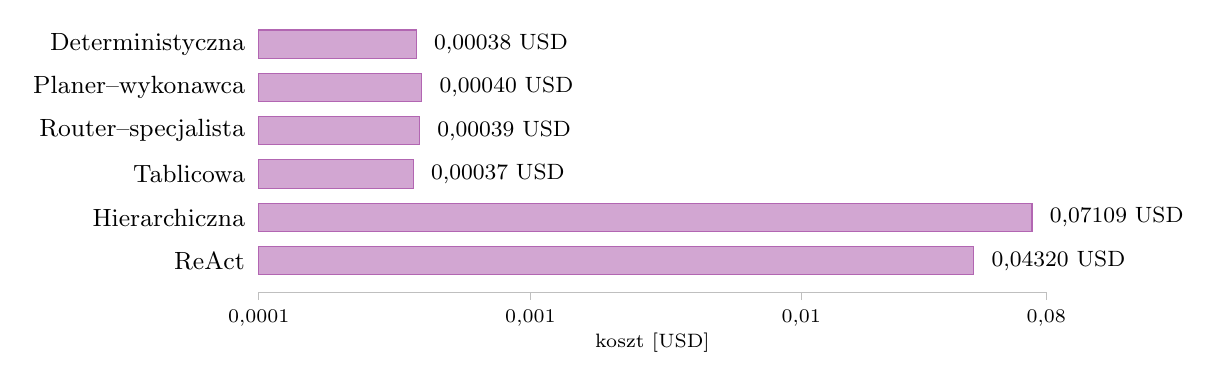
\begin{tikzpicture}[
        archlbl/.style={font=\small, anchor=east, inner sep=2pt},
        valuelbl/.style={font=\footnotesize, anchor=west, inner sep=2pt},
        ticklbl/.style={font=\scriptsize, anchor=north},
        baraxis/.style={draw=gray!50, line width=0.3pt}
      ]
      \def\bw{10}
      \def\bh{0.18}
      \foreach \name/\barlen/\lbl/\y in {%
        Deterministyczna/2.00/0{,}00038~USD/0,
        Planer--wykonawca/2.07/0{,}00040~USD/-0.55,
        Router--specjalista/2.04/0{,}00039~USD/-1.10,
        Tablicowa/1.96/0{,}00037~USD/-1.65,
        Hierarchiczna/9.82/0{,}07109~USD/-2.20,
        ReAct/9.08/0{,}04320~USD/-2.75%
      }{
        \node[archlbl] at (-0.1,\y) {\name};
        \fill[violet!35, draw=violet!60]
        (0,\y-\bh) rectangle (\barlen,\y+\bh);
        \node[valuelbl] at ({\barlen+0.15},\y) {\lbl};
      }
      \draw[baraxis] (0,-3.15) -- (\bw,-3.15);
      \foreach \v/\lbl in {
      0/0{,}0001, 3.45/0{,}001, 6.89/0{,}01, 10/0{,}08} {
        \draw[baraxis] (\v,-3.15) -- (\v,-3.25);
        \node[ticklbl] at (\v,-3.25) {\lbl};
      }
      \node[font=\scriptsize, anchor=north] at (5,-3.55) {koszt [USD]};
    \end{tikzpicture}
  \end{adjustbox}
  \zrodlo{opracowanie własne}
\end{wykres}

Dla architektury hierarchicznej koszt jest funkcją rekurencyjnego rozkładu
pytań. Każde podpytanie generuje własny pełny przebieg pobierania, syntezy
i~oceny, a~łączna liczba wywołań narzędzi osiąga średnio 1\,066 na uruchomienie
-- przy odchyleniu standardowym 2\,568, co wskazuje na wysoką wariancję
kosztową tej architektury. Zarejestrowane ścieżki wykonania wskazują, że dla
części pytań długość kontekstu zbliżała się do progu okna modelu, co dodatkowo
obniżało jakość syntezy.

W~architekturze ReAct koszt rośnie wraz z~liczbą iteracji kontrolera. Ustalony
limit 15~iteracji nie został osiągnięty w~żadnym z~przebiegów -- maksymalna
odnotowana liczba iteracji wyniosła~11, a~6~przebiegów osiągnęło 10~lub więcej
iteracji. Każda iteracja uruchamiała odrębne wywołanie narzędzia pobierającego
fragmenty -- stąd średnio 295{,}7 wywołań na pytanie wobec 7{,}2 dla
planera--wykonawcy. Architektura ta charakteryzuje się jednocześnie największą
wariancją opóźnienia, co w~środowisku produkcyjnym stwarza ryzyko przekroczenia
limitów czasowych interfejsu użytkownika. Podobnie jak w~przypadku architektury
hierarchicznej, wariancja zużycia tokenów w~architekturze ReAct przekracza
wartość jej średniej (odchylenie standardowe 419\,373 przy średniej 391\,935
tokenów wejściowych). Stan ten jednoznacznie wskazuje na prawostronnie skośny
rozkład kosztu operacyjnego -- znaczna większość pytań jest rozwiązywana bez
trudu, jednak sporadyczne wpadnięcie agenta w~wielokrotne pętle lub powielane
halucynacje pochłania skrajne zasoby obliczeniowe i~staje się źródłem potężnego
zawyżenia średnich wydatków na utrzymanie aplikacji.

Nie stwierdzono korelacji między kosztem a~jakością. Warianty iteracyjne,
wymagające przetworzenia ponad stukrotnie większej liczby tokenów, osiągają
niższe wyniki w~każdej z~czterech miar jakości niż najtańszy wariant
z~pierwszej grupy.

\section{Wnioski jakościowe}\label{sec:wnioski-jakosciowe}

Analiza jakościowa rozszerza pomiary statystyczne o~identyfikację powtarzalnych
wzorców błędów wynikających ze struktury dokumentów i~specyfiki działania
poszczególnych architektur. Badaniu poddano przebiegi o~najniższych wynikach
wierności i~poprawności, wyodrębnione na podstawie plików wynikowych opisanych
w~sekcji~\ref{subsec:artefakty-wynikowe}.

\subsection{Charakterystyka niepowodzeń}\label{subsec:charakterystyka-niepowodzen}

Analiza odpowiedzi o~najniższej wierności i~poprawności pozwala wyodrębnić
powtarzalne mechanizmy błędów. Część odpowiedzi poprawnie przytacza dany fakt,
lecz omija klauzulę wyłączenia lub warunek ograniczający ochronę -- ich treść
pozostaje zgodna z~kontekstem, lecz niekompletna wobec odpowiedzi
referencyjnej. W~pozostałych przebiegach zasadnicza treść odpowiedzi jest
poprawna, jednak dołączony szczegół -- na przykład wartość liczbowa lub nazwa
wariantu produktu -- nie posiada pokrycia w~pobranych fragmentach. Trzecią
grupę stanowią odpowiedzi, w~których pojedyncze stwierdzenia wynikają
z~pobranych fragmentów, lecz ich kombinacja odnosi się do różnych produktów lub
ubezpieczycieli, co prowadzi do błędnego przedstawienia zakresu ochrony.

Zidentyfikowane profile błędów są zróżnicowane w~zależności od architektury.
W~przebiegach wariantów deterministycznego i~tablicowego dominują odpowiedzi
niepełne -- klauzule wyłączeń są omijane przy jednoczesnej poprawności
pozostałej treści. W~przebiegach routera--specjalisty i~planera--wykonawcy
częściej obserwuje się uzupełnienie poprawnej treści o~niepotwierdzone
szczegóły. Architektury hierarchiczna i~ReAct wykazują oba te zjawiska --
rozbudowują odpowiedź i~jednocześnie łączą fragmenty dotyczące różnych
produktów. Uzyskane wyniki pozwalają zgrupować badane architektury w~trzy pary
na podstawie dominującego typu błędu: deterministyczna i~tablicowa generują
odpowiedzi niepełne, router--specjalista i~planer--wykonawca odpowiedzi
nadbudowane, natomiast hierarchiczna i~ReAct odpowiedzi o~niejednolitym
kontekście produktowym.

Z~perspektywy regulacyjnej rodzaj generowanych błędów posiada istotne
implikacje praktyczne. Odpowiedź niepełna sygnalizuje niedobór informacji, co
umożliwia użytkownikowi sformułowanie pytań doprecyzujących. Odpowiedzi
z~nadbudowaną treścią lub połączonymi fragmentami stwarzają pozory
kompletności, mimo że przekazują błędne informacje o~zakresie ochrony. Powyższe
obserwacje uzasadniają wybór architektur o~prostszym i~bardziej
deterministycznym przepływie sterowania w~zastosowaniach, w~których ryzyko
wprowadzenia w~błąd użytkownika stanowi koszt wyższy niż dostarczenie
odpowiedzi niekompletnej.

\subsection{Systematyczne pomijanie klauzul wyłączeń}\label{subsec:systematyczne-pomijanie-klauzul-wylaczen}

Najczęstszym mechanizmem odpowiedzi niepełnych jest pomijanie klauzul wyłączeń
przez warstwę pobierania. Dokumenty OWU charakteryzują się asymetryczną
strukturą językową: klauzule pokrycia zaczynają się od sformułowań
afirmatywnych (,,ubezpieczyciel pokrywa szkody powstałe wskutek...''),
a~klauzule wyłączeń od sformułowań negatywnych (,,ubezpieczyciel nie ponosi
odpowiedzialności, jeśli...''). Zapytania użytkowników sformułowane są
przeważnie w~formie twierdzącej, w~wyniku czego podobieństwo kosinusowe między
pytaniem a~klauzulami wyłączeń jest niższe niż podobieństwo względem klauzul
ochrony.

Omawiane zjawisko występuje we~wszystkich badanych architekturach. Ograniczenie
to wynika z~metody reprezentacji wektorowej i~nie zależy od przyjętej topologii
sterowania. Warianty iteracyjne, mimo większej liczby wywołań narzędzi, nie
redukują tego zjawiska -- dryf semantyczny powoduje, że kolejne zapytania
pozostają w~afirmatywnym rejestrze i~jedynie poszerzają jego zakres.

\subsection{Niedobór kontekstu definicyjnego}\label{subsec:niedobor-kontekstu-definicyjnego}

Drugim mechanizmem jest pominięcie przez moduł wyszukiwania sekcji definiującej
termin użyty w~klauzuli docelowej. W~polskich dokumentach OWU definicje
znajdują się w~sekcjach wstępnych, natomiast zdefiniowane terminy występują
w~klauzulach umieszczonych w~dalszych częściach tekstu. Zapytanie użytkownika
jest semantycznie bliższe klauzuli użycia, wobec czego wyszukiwanie zwraca tę
klauzulę i~pomija sekcję definicyjną. Odpowiedź pozostaje wierna wobec
pobranego fragmentu, jednak brak kontekstu pojęciowego skutkuje odpowiedzią
niepełną z~perspektywy użytkownika.

Wzorzec ten odpowiada za znaczną część rozbieżności między wiernością
a~poprawnością -- architektura uzyskuje wysoką wierność przy jednocześnie
niskiej poprawności, ponieważ pobrany kontekst jest niekompletny względem
odpowiedzi referencyjnej.

\subsection{Bezwarunkowa dekompozycja w~architekturze hierarchicznej}\label{subsec:bezwarunkowa-dekompozycja-w-architekturze-hierarchicznej}

W~architekturze hierarchicznej zaobserwowano powtarzalny wzorzec bezwarunkowej
dekompozycji pytań jednoaspektowych. Węzeł dekompozytora uruchamiany jest
niezależnie od charakteru pytania, przez co nawet proste pytania są rozkładane
na podpytania. Każde podpytanie inicjuje osobny przebieg pobierania, a~węzeł
scalający uzupełnia wynikową odpowiedź elementami z~wiedzy parametrycznej
modelu tam, gdzie wśród pobranych fragmentów brakuje bezpośredniej odpowiedzi.

Skutkuje to najniższą wiernością dla pytań bardzo prostych: 0{,}556 wobec
0{,}889 architektury deterministycznej. Węzeł dekompozytora powinien działać
warunkowo, po uprzedniej klasyfikacji pytania według stopnia złożoności --
w~zbadanej implementacji warunek ten nie był spełniony.

\subsection{Rozszerzanie zakresu wyszukiwania w~architekturze ReAct}\label{subsec:rozszerzanie-zakresu-wyszukiwania-w-architekturze-react}

W~architekturze ReAct zaobserwowano zjawisko narastającego rozszerzania zakresu
wyszukiwania w~kolejnych iteracjach pętli. W~przypadku otrzymania
niejednoznacznej obserwacji kontroler generuje zapytanie ogólniejsze niż
poprzednie. W~efekcie zapytania o~konkretny produkt zaczynają obejmować
produkty powiązanych ubezpieczycieli, zwracając fragmenty tematycznie zbliżone,
lecz produktowo odmienne. Wygenerowane odpowiedzi zawierają stwierdzenia
poparte poszczególnymi fragmentami, lecz ich kombinacja łączy postanowienia
różnych polis. Wyjątkową podatność na ten błąd zaobserwowano dla pytań z~kategorii
ubezpieczeń mieszkaniowych, w~której wierność ReAct drastycznie spadła do
zaledwie 0{,}433 -- zjawisko dryfu uderza najsilniej tam, gdzie pojęcia
dziedzinowe posiadają najszerszy i~podatny na wieloznaczność kontekst.

Zjawisko to jest trudne do wykrycia przez automatyczną ocenę opartą na
weryfikacji obecności twierdzeń w~kontekście -- odpowiedź nie wykracza
formalnie poza pobrany zbiór, jednakże pozostaje niepoprawna z~perspektywy
zapytania.

\subsection{Niespójność autorytetu między OWU a~IPID}\label{subsec:niespojnosc-autorytetu-miedzy-owu-a-ipid}

W~kilku zarejestrowanych przypadkach wyszukiwanie zwróciło jednocześnie
fragment IPID z~zaokrągloną wartością sumy ubezpieczenia oraz fragment OWU
z~dokładną wartością umowną. Selektor dowodów, działający na podobieństwie
kosinusowym, ocenił fragment IPID jako bliższy pytaniu -- formularz IPID jest
zwięzły i~osiąga wyższe podobieństwo do prostych zapytań użytkowników. Synteza
odtworzyła wartość zaokrągloną. Odpowiedź była wierna wobec pobranego
kontekstu, lecz niezgodna z~wiążącym dokumentem umownym.

Mechanizm ten jest niezależny od architektury sterowania -- wystąpił we
wszystkich sześciu wariantach. Wynika on z~umieszczenia obu typów dokumentów
w~jednej kolekcji wektorowej bez metadanowego oznaczenia hierarchii autorytetu.

\subsection{Samokorekta w~architekturze tablicowej}\label{subsec:samokorekta-w-architekturze-tablicowej}

W~architekturze tablicowej zaobserwowano mechanizm samokorekty. W~pojedynczych
przypadkach moduł przepisywania zapytań zwrócił ucięty wynik (odpowiedź modelu
osiągnęła limit tokenów przed zamknięciem formatu \texttt{JSON}), pozostawiając
pole \texttt{rewritten\_queries} stanu grafu puste. W~architekturze
deterministycznej taka sytuacja propagowała się bez korekty. W~architekturze
tablicowej dyspozytor wykrył puste pole i~ponownie wywołał moduł przepisywania.

Mechanizm ten wynika z~ogólnej reguły dyspozytora: w~przypadku pustego pola,
należy uruchomić odpowiedniego agenta. Jest to przykład samokorekty wynikającej
z~topologii, a~nie z~jawnej obsługi błędów. W~środowisku produkcyjnym taka
odporność na awarie narzędzi posiada znaczną wartość operacyjną,
nieproporcjonalną do kosztu jej zaimplementowania.

\section{Rozstrzygnięcie problemu badawczego i~realizacja celów}\label{sec:odpowiedz-na-pytania-badawcze-i-realizacja-celow}

Sekcja zestawia sformułowane wnioski najpierw z~głównym problemem badawczym,
a~następnie z~pytaniami badawczymi PB1--PB4 i~celami CB1--CB4
z~\cref{chap:wprowadzenie}.

\subsection{Rozstrzygnięcie głównego problemu badawczego}\label{subsec:glowny-problem-badawczy}

Główny problem badawczy pracy wynikał z~braku kontrolowanego porównania
topologii agentowych oraz pytania, czy bardziej złożone systemy wieloagentowe
oferują lepszą jakość odpowiedzi niż prostsze układy jednoagentowe
w~identycznym środowisku testowym. Uzyskane wyniki nie pozwalają na
sformułowanie jednoznacznej odpowiedzi. Wskazują one natomiast, że sama
opozycja jednoagentowe--wieloagentowe nie stanowi wystarczającego kryterium
oceny jakości: złożoność topologii przynosi korzyść tylko wtedy, gdy poprawia
dobór kontekstu lub sterowanie przebiegiem bez wprowadzania nadmiernego narzutu
iteracyjnego.

Najwyższą wierność uzyskał router--specjalista, co wskazuje, że dodatkowy
mechanizm trasowania może poprawić jakość odpowiedzi w~najtrudniejszych
przypadkach. Jednocześnie najwyższą poprawność osiągnęła architektura
deterministyczna, a~najbardziej kosztowne warianty iteracyjne -- hierarchiczna
i~ReAct -- nie uzyskały lepszych wyników pomimo większej liczby kroków
rozumowania. Rozstrzygnięcie głównego problemu badawczego ma zatem charakter
warunkowy: większa złożoność architektury nie gwarantuje automatycznej przewagi
jakościowej, lecz wybrane mechanizmy sterowania, w~tym szczególnie trasowanie
zapytań, mogą być użyteczne, jeśli pozostają ściśle powiązane z~warstwą
pobierania dokumentów.

\subsection{Wpływ topologii na jakość odpowiedzi}\label{subsec:wplyw-topologii-na-jakosc-odpowiedzi}

Wartości wierności dla poszczególnych architektur zawierają się w~przedziale
0{,}611--0{,}811, a~wartości poprawności w~przedziale 0{,}588--0{,}716.
Najwyższą wierność osiąga router--specjalista (0{,}811), najwyższą poprawność
architektura deterministyczna (0{,}716). Żadna architektura nie dominuje
jednocześnie we~wszystkich czterech miarach; przewagi są specyficzne dla miary
i~poziomu trudności pytania.

Hipoteza PB1, zakładająca przewagę bardziej złożonych topologii, znajduje tylko
częściowe potwierdzenie. Najwyższą wierność osiąga router--specjalista, a~trzy
z~pięciu topologii bardziej złożonych niż deterministyczna uzyskują wierność
nie niższą od wariantu bazowego. Jednocześnie hierarchiczna i~ReAct pokazują,
że sama złożoność orkiestracji nie gwarantuje wzrostu jakości: ich wyniki są
niższe mimo większej liczby kroków i~wywołań narzędzi.

\subsection{Kompromis między jakością a~kosztem}\label{subsec:kompromis-miedzy-jakoscia-a-kosztem}

W~ramach analizowanego zadania nie zaobserwowano kompromisu między jakością
odpowiedzi a~kosztem operacyjnym. Cztery architektury o~stałym lub płytko
sterowanym przebiegu uzyskują wyższe wyniki w~większości miar jakości przy
koszcie 0{,}00037--0{,}00040~USD na pytanie. Koszty wariantów iteracyjnych
wynoszą odpowiednio 0{,}04320~USD i~0{,}07109~USD na uruchomienie, co wiąże się
jednocześnie z~niższą wiernością i~poprawnością. Stosunek kosztu architektury
hierarchicznej do deterministycznej wynosi 187, ReAct do deterministycznej --
114.

Na poziomie pytań bardzo złożonych router--specjalista i~tablicowa uzyskują po
0{,}815 wierności, natomiast wynik architektury hierarchicznej spada do
0{,}593. Hipoteza PB2 o~braku proporcjonalnego wzrostu jakości wraz z~kosztem
orkiestracji znajduje potwierdzenie, przy czym wyniki doprecyzowują ją:
największy narzut kosztowy wynika z~iteracyjnej kontroli przebiegu, a~nie
z~samego wprowadzenia dodatkowej roli lub klasyfikatora.

\subsection{Wpływ planowania, trasowania i~dekompozycji}\label{subsec:wplyw-planowania-trasowania-i-dekompozycji}

Dodanie warstwy planowania przyniosło nieoczekiwany paradoks
wydajnościowy -- architektura planera--wykonawcy okazała się najszybsza
czasowo dzięki trafnej redukcji wywołań narzędzi (7{,}2 wobec 10,0 w~wariancie
deterministycznym). Sukces ten jest jednak obarczony anomalią iluzji filtrowania
dowodów: po ocenie trafności w~stanie pozostaje zaledwie 0{,}31 fragmentu na
zapytanie, podczas gdy węzeł syntezy wciąż generuje 3{,}38 cytowania, jawnie
ignorując wyniki sędziego.

Z~kolei mechanizmy planowania i~bezwarunkowej dekompozycji nie zapewniają
systematycznej poprawy wyników dla pytań złożonych ani bardzo złożonych.
Najwyższe wyniki dla pytań bardzo złożonych osiągają architektury bez
iteracyjnej kontroli (router--specjalista i~tablicowa, po~0{,}815 wierności).
Spośród mechanizmów analizowanych w~PB3 jedynie trasowanie wykazuje ograniczoną
przewagę -- na poziomie pytań bardzo złożonych router--specjalista osiąga
0{,}815 wobec 0{,}704 w~architekturze deterministycznej (różnica 0{,}111
punktu).

Dekompozycja hierarchiczna pogarsza wynik na każdym poziomie trudności,
najwyraźniej dla pytań prostych, z~przyczyny opisanej
w~sekcji~\ref{subsec:bezwarunkowa-dekompozycja-w-architekturze-hierarchicznej}.

\subsection{Wzorce niepowodzeń}\label{subsec:wzorce-niepowodzen}

Architektury wykazują odmienne profile niepowodzeń, opisane
w~sekcji~\ref{subsec:charakterystyka-niepowodzen}. Architektury
deterministyczna i~tablicowa generują błędy polegające na pomijaniu klauzul
wyłączeń, router--specjalista i~planer--wykonawca -- na uzupełnianiu poprawnego
rdzenia o~niepotwierdzony szczegół, natomiast hierarchiczna i~ReAct -- łączą
oba zjawiska, dodatkowo mieszając fragmenty z~różnych produktów. Hipoteza
o~zróżnicowanych profilach błędów znajduje pełne potwierdzenie.

\subsection{Odpowiedzi na pytania badawcze}\label{subsec:odpowiedzi-na-pytania-badawcze}

Wszystkie cztery pytania badawcze sformułowane w~\cref{chap:wprowadzenie}
zostały empirycznie rozstrzygnięte. Pytanie PB1 rozstrzygnięto częściowo
względem hipotezy o~przewadze bardziej złożonych topologii: najwyższą wierność
uzyskał router--specjalista, lecz rozkład wyników wskazuje, że przewaga nie
wynika z~samej złożoności, lecz z~konkretnego mechanizmu sterowania
pobieraniem. Rozstrzygnięcie PB2 oparto na obserwacji, że warianty iteracyjne
generują koszt rzędu 100--187 razy wyższy niż architektury o~stałym lub płytko
sterowanym przebiegu, przy jednocześnie niższych wynikach w~każdej z~miar
jakości -- w~zbadanym zadaniu zwiększanie nakładu obliczeniowego nie przekłada
się proporcjonalnie na jakość. Pytanie PB3 rozstrzygnięto częściowo: trasowanie
wnosi mierzalną, choć ograniczoną przewagę na pytaniach bardzo złożonych,
podczas gdy bezwarunkowa dekompozycja i~iteracyjne planowanie konsekwentnie
pogarszają wynik. Pytanie PB4 rozstrzygnięto twierdząco -- architektury
rozdzielają się na trzy odrębne profile niepowodzeń sparowane po dwie
konfiguracje, co potwierdza, że topologia sterowania determinuje charakter
typowego błędu w~większym stopniu niż jego częstość.
Tabela~\ref{tab:odpowiedzi-na-pytania-badawcze} podsumowuje wnioski płynące
z~rozstrzygnięcia poszczególnych pytań.

\begin{table}[H]
  \caption{Odpowiedzi na pytania badawcze}\label{tab:odpowiedzi-na-pytania-badawcze}
  \centering
  \small
  \renewcommand{\arraystretch}{1.3}
  \begin{tabularx}{\textwidth}{@{} l X @{}}
    \toprule
    \textbf{Pytanie} & \textbf{Wniosek}                                                         \\
    \midrule
    PB1
    & Najwyższa wierność routera--specjalisty; przewaga złożoności częściowa
    i~zależna od konkretnego mechanizmu sterowania.                                             \\
    PB2
    & Brak proporcjonalnego związku jakość--koszt; warianty iteracyjne droższe
    i~gorsze jakościowo.                                                                        \\
    PB3
    & Trasowanie daje ograniczoną przewagę na pytaniach bardzo złożonych;
    dekompozycja pogarsza wynik.                                                                \\
    PB4
    & Trzy odrębne profile niepowodzeń; architektury grupują się parami
    według dominującego mechanizmu.                                                             \\
    \bottomrule
  \end{tabularx}
  \zrodlo{opracowanie własne}
\end{table}

\subsection{Realizacja celów badawczych}\label{subsec:realizacja-celow-badawczych}

Wszystkie cztery cele badawcze zostały zrealizowane. Środowisko orkiestracji
oparte na \texttt{LangGraph} i~\texttt{Arize Phoenix} umożliwiło uruchomienie
sześciu architektur w~jednym przebiegu na identycznym indeksie wektorowym
i~przy wspólnej warstwie narzędzi (CB1). Dedykowany zestaw 90~pytań testowych
związanych z~polskojęzycznymi dokumentami OWU i~IPID powstał na potrzeby
eksperymentu (CB2). Ewaluacja wszystkich sześciu architektur z~wykorzystaniem
czterech miar jakości i~zestawu miar operacyjnych stanowi realizację celu CB3.
Analiza zebranych danych z~rozróżnieniem profili niepowodzeń każdej
architektury oraz rekomendacje praktyczne dla zespołów wdrożeniowych realizują
CB4, którego konkluzja stanowi rozstrzygnięcie głównego problemu badawczego:
złożoność architektury przynosi korzyść wtedy, gdy służy precyzyjnemu
sterowaniu pobieraniem, lecz iteracyjna dekompozycja i~ReAct nie zapewniają
wyższej jakości pomimo większego nakładu.

\section{Kierunki dalszych badań}\label{sec:kierunki-dalszych-badan}

Wyniki eksperymentu wskazują kilka potencjalnych kierunków kontynuacji badań,
wynikających z~ograniczeń zaobserwowanych w~zbadanym układzie.

Pierwszym kierunkiem jest rozszerzenie zestawu testowego do co najmniej
220~pytań przy udziale co najmniej dwóch modeli bazowych od różnych dostawców.
Obecna próba 90~pytań nie pozwala statystycznie rozróżnić różnic między
czterema najtańszymi architekturami (rozpiętość 0{,}033 punktu wierności).
Drugi model bazowy pozwoliłby ocenić, w~jakim stopniu obserwowane wzorce są
specyficzne dla \texttt{gpt-5}, a~w~jakim wynikają z~samej topologii.

Drugim kierunkiem jest opracowanie strategii wyszukiwania uwzględniających
asymetrię polaryzacji semantycznej między klauzulami pokrycia a~klauzulami
wyłączeń. Jednym z~możliwych rozwiązań jest wyszukiwanie hybrydowe łączące
podobieństwo gęste z~indeksem leksykalnym \texttt{BM25} oraz osadzenia
asymetryczne trenowane na parach pytanie--klauzula z~odwróconą polaryzacją.
Niezależną ścieżką jest metadanowe oznaczenie roli klauzuli w~indeksie
i~wymuszenie pobierania zarówno klauzul pokrycia, jak i~wyłączeń dla każdego
pytania o~zakres ochrony.

Trzecim kierunkiem jest segmentacja dokumentów oparta na strukturze prawnej,
a~nie na progu liczby tokenów. W~roli granic fragmentów należy wykorzystać
granice ustępów, podpunktów lub klauzul, co zmniejsza ryzyko łączenia
merytorycznie niezwiązanych zapisów w~jednym fragmencie. Wstępna analiza
indeksu wskazuje, że fragmenty o~rozmiarze 256~tokenów z~podziałem klauzulowym
mogą podnieść trafność dokumentów niezależnie od architektury.

Czwartym kierunkiem jest weryfikacja automatycznej ewaluacji przez ekspertów
dziedzinowych. Próba 200--300~ocen przeprowadzonych przez prawnika lub
specjalistę do spraw oceny ryzyka pozwoliłaby zmierzyć korelację między oceną
sędziego opartego na modelu a~oceną merytoryczną oraz oszacować systematyczne
obciążenia tej formy ewaluacji w~kontekście prawno-umownym.

Piątym kierunkiem jest ocena mechanizmów planowania, trasowania i~dekompozycji
w~zadaniach wymagających rzeczywistego wnioskowania wieloskokowego -- takich,
w~których odpowiedź wymaga zestawienia klauzul z~dokumentów różnych
ubezpieczycieli. W~obecnym zestawie każde pytanie dotyczyło jednego produktu,
co uniemożliwiło ujawnienie ewentualnej przewagi mechanizmów dekompozycji.
Zadania wielodokumentowe stanowią środowisko, w~którym hipoteza o~przewadze
bardziej złożonych topologii mogłaby zostać zweryfikowana w~środowisku
o~wyższym stopniu złożoności.

\section{Rekomendacje dla praktyków}\label{sec:rekomendacje-dla-praktykow}

Niniejsza sekcja skierowana jest do inżynierów projektujących produkcyjne
systemy odpowiadania na pytania na podstawie dokumentów regulacyjnych.
Zalecenia zostały uporządkowane według hierarchii priorytetów, a~ich
szczegółowy zestaw zebrano
w~tabeli~\ref{tab:rekomendacje-dla-wdrozen-produkcyjnych}.

Najwyższy wpływ na poprawę wyników wykazuje optymalizacja indeksu --
segmentacja klauzulowa, oddzielne kolekcje OWU i~IPID oraz metadanowe
oznaczenie roli klauzuli (pokrycie, wyłączenie, definicja) eliminują źródła
błędów wspólne dla wszystkich badanych architektur. Drugą warstwą jest
strategia pobierania (wyszukiwanie hybrydowe, osadzenia asymetryczne, wymuszone
pobieranie wyłączeń). Wybór topologii agentowej stanowi trzeci poziom
priorytetu -- w~zbadanym zadaniu różnice między czterema najtańszymi
architekturami mieszczą się w~granicach niepewności pomiarowej. Wybór modelu
bazowego ma marginalne znaczenie, pod warunkiem że model spełnia minimalne
wymagania jakości syntezy w~języku polskim.

\begin{table}[H]
  \caption{Rekomendacje dla wdrożeń produkcyjnych}\label{tab:rekomendacje-dla-wdrozen-produkcyjnych}
  \centering
  \small
  \renewcommand{\arraystretch}{1.3}
  \begin{tabularx}{\textwidth}{@{} l X @{}}
    \toprule
    \textbf{Rekomendacja} & \textbf{Uzasadnienie}                                                                           \\
    \midrule
    Wariant bazowy
    & Architektura deterministyczna: najprostsza analiza niepowodzeń; najwyższa poprawność (0{,}716);
    profil błędów ukierunkowany na odpowiedzi niepełne zamiast
    halucynacji, wiążący się z~niższym ryzykiem w~kontekście regulacyjnym.                                                  \\
    Trasowanie warunkowo
    & Przewaga 0{,}111 punktu wierności na pytaniach bardzo złożonych;
    koszt dodatkowego wywołania klasyfikatora pomijalny.                                                                    \\
    Oddzielne kolekcje OWU i~IPID
    & Eliminuje niespójność autorytetu między wartością umowną
    a~zaokrągloną, opisaną w~sekcji~\ref{subsec:niespojnosc-autorytetu-miedzy-owu-a-ipid}.                                  \\
    Segmentacja klauzulowa
    & Granice fragmentów na poziomie ustępów i~klauzul;
    docelowy rozmiar 256~tokenów.                                                                                           \\
    Indeksowanie wyłączeń
    & Metadanowe oznaczenie roli klauzuli i~wymuszenie pobierania
    zarówno klauzul pokrycia, jak i~wyłączeń.                                                                               \\
    Pominięcie wariantów iteracyjnych
    & Brak wnioskowania wieloskokowego w~zadaniu;
    koszt 100--187-krotnie wyższy przy jednoczesnym braku wzrostu jakości.                                                  \\
    Regresyjny zestaw kontrolny
    & Zmiana modelu po stronie dostawcy może zmienić wyniki bez
    modyfikacji kodu; zalecane cykliczne uruchamianie 30--50~pytań.                                                         \\
    Przegląd ekspercki
    & 20--30~odpowiedzi miesięcznie weryfikowanych przez prawnika
    lub specjalistę; sygnał o~dryfcie jakości niewidocznym dla
    sędziego opartego na modelu językowym.                                                                                  \\
    \bottomrule
  \end{tabularx}
  \zrodlo{opracowanie własne}
\end{table}

\section{Zakończenie}\label{sec:zakonczenie}

Praca dotyczyła empirycznej weryfikacji wpływu topologii systemu agentowego
i~jej złożoności na jakość odpowiedzi generowanych na podstawie obszernych
dokumentów regulacyjnych. Uzyskane wyniki pozwalają na doprecyzowanie hipotezy
wyjściowej: przewagę uzyskują topologie, w~których pojedynczy przebieg
pobierania jest precyzyjnie ukierunkowany, a~nie te, które wykonują największą
liczbę kroków rozumowania.

Cztery architektury bez rozbudowanej pętli iteracyjnej osiągają wierność
w~przedziale 0{,}778--0{,}811 przy koszcie 0{,}00037--0{,}00040~USD na pytanie.
Dwa warianty iteracyjne generują ponad stukrotnie wyższe koszty i~jednocześnie
uzyskują niższe wyniki w~każdej z~czterech miar jakości. Zależność ta nie
potwierdza hipotezy o~bezpośredniej przewadze jakościowej wynikającej ze
złożoności orkiestracji, ale wskazuje na warunkową przydatność wybranych
mechanizmów złożoności, zwłaszcza trasowania.

W~ramach niniejszej pracy zrealizowano cztery główne wkłady badawcze. Pierwszym
z~nich jest odtwarzalna platforma porównawcza sześciu architektur agentowych
działających w~identycznym środowisku, na tych samych danych i~przy tej samej
infrastrukturze ewaluacyjnej. Drugim jest oryginalny zestaw testowy 90~pytań do
polskojęzycznych dokumentów ubezpieczeniowych. Trzecim jest opis powtarzalnych
wzorców błędów z~rozróżnieniem profili ryzyka -- odpowiedź niepełna wiąże się
z~niższym ryzykiem niż odpowiedź halucynacyjna wykazująca pozorną kompletność
w~kontekście regulacyjnym. Czwartym jest empiryczne doprecyzowanie problemu
złożoności topologii: sama liczba ról, kroków lub iteracji nie determinuje
o~jakości, natomiast ukierunkowane sterowanie pobieraniem może poprawiać wynik
w~najtrudniejszych pytaniach.

W~środowisku regulacyjnym błędy w~odpowiedziach systemu niosą za sobą istotne
implikacje praktyczne. Wyniki niniejszej pracy wskazują, że budowa wiarygodnych
systemów odpowiadania na pytania w~tej domenie jest możliwa przy stosunkowo
prostej, precyzyjnie sterowanej architekturze -- pod warunkiem, że priorytetem
jest jakość warstwy pobierania, indeksowanie klauzul wyłączeń i~hierarchia
autorytetu między typami dokumentów, a~nie liczba kroków rozumowania.

\listoftables
\addcontentsline{toc}{chapter}{Wykaz tabel}

\listoffigures
\addcontentsline{toc}{chapter}{Wykaz rysunk\'ow}

\listof{wykres}{Wykaz wykres\'ow}
\addcontentsline{toc}{chapter}{Wykaz wykres\'ow}

\printbibliography[title={Bibliografia}, heading=bibintoc]

\appendix
\chapter{Prompty systemu}\label{app:prompty}

Dodatek zawiera moduł \texttt{sources/config/prompts.py} z~promptami
wykorzystywanymi w~systemie. Ich wydzielenie zwiększa czytelność opisu
implementacji w~rozdziale~\ref{chap:implementacja} i~umożliwia weryfikację
treści instrukcji przekazywanych modelom.

\lstdefinestyle{promptlisting}{
  language=Python,
  basicstyle=\ttfamily\tiny,
  breaklines=true,
  breakatwhitespace=true,
  columns=fullflexible,
  keepspaces=true,
  showstringspaces=false,
  literate=
  {ą}{{\k{a}}}1 {ę}{{\k{e}}}1 {ó}{{\'o}}1 {ś}{{\'s}}1
  {ł}{{\l{}}}1 {ż}{{\.z}}1 {ź}{{\'z}}1 {ć}{{\'c}}1 {ń}{{\'n}}1
  {Ą}{{\k{A}}}1 {Ę}{{\k{E}}}1 {Ó}{{\'O}}1 {Ś}{{\'S}}1
  {Ł}{{\L{}}}1 {Ż}{{\.Z}}1 {Ź}{{\'Z}}1 {Ć}{{\'C}}1 {Ń}{{\'N}}1
  {§}{{\S{}}}1 {—}{{--}}1
  {✓}{{\checkmark}}1 {✗}{{\(\times\)}}1,
}

Prompt \texttt{EXTRACTION\_PROMPT} służy jako instrukcja systemowa dla modelu
multimodalnego podczas ekstrakcji tekstu ze stron dokumentów ubezpieczeniowych
metodą OCR.

\lstinputlisting[
  style=promptlisting,
  firstline=13,
  lastline=45,
  caption={Prompt ekstrakcji tekstu OCR (\texttt{EXTRACTION\_PROMPT})},
  label={lst:app-extraction-prompt}
]{../code/sources/config/prompts.py}

Prompt \texttt{QUESTION\_PARSER\_SYSTEM\_PROMPT} definiuje proces wyodrębniania
strukturalnych metadanych z~pytania użytkownika na potrzeby filtrowania w~bazie
wektorowej Qdrant.

\lstinputlisting[
  style=promptlisting,
  firstline=47,
  lastline=96,
  caption={Prompt parsera pytań (\texttt{QUESTION\_PARSER\_SYSTEM\_PROMPT})},
  label={lst:app-question-parser-prompt}
]{../code/sources/config/prompts.py}

Prompt \texttt{QUERY\_REWRITER\_SYSTEM\_PROMPT} służy do generowania trzech
zróżnicowanych leksykalnie wariantów zapytania na potrzeby wyszukiwania
wektorowego.

\lstinputlisting[
  style=promptlisting,
  firstline=98,
  lastline=117,
  caption={Prompt przepisania zapytań (\texttt{QUERY\_REWRITER\_SYSTEM\_PROMPT})},
  label={lst:app-query-rewriter-prompt}
]{../code/sources/config/prompts.py}

Prompt \texttt{RERANKER\_SYSTEM\_PROMPT} definiuje kryteria dla modelu
oceniającego trafność każdego pobranego fragmentu dokumentu względem zadanego
pytania w~skali 0--1.

\lstinputlisting[
  style=promptlisting,
  firstline=119,
  lastline=140,
  caption={Prompt oceny trafności fragmentów (\texttt{RERANKER\_SYSTEM\_PROMPT})},
  label={lst:app-reranker-prompt}
]{../code/sources/config/prompts.py}

Prompt \texttt{REFERENCE\_CORRECTNESS\_PROMPT} jest wykorzystywany przez
ewaluator Phoenix do oceny poprawności wygenerowanej odpowiedzi względem
wzorcowej odpowiedzi referencyjnej.

\lstinputlisting[
  style=promptlisting,
  firstline=142,
  lastline=175,
  caption={Prompt oceny poprawności odpowiedzi (\texttt{REFERENCE\_CORRECTNESS\_PROMPT})},
  label={lst:app-reference-correctness-prompt}
]{../code/sources/config/prompts.py}

Prompt \texttt{CONCISENESS\_PROMPT} jest używany przez ewaluator Phoenix do
oceny zwięzłości odpowiedzi generowanej przez system.

\lstinputlisting[
  style=promptlisting,
  firstline=177,
  lastline=210,
  caption={Prompt oceny zwięzłości odpowiedzi (\texttt{CONCISENESS\_PROMPT})},
  label={lst:app-conciseness-prompt}
]{../code/sources/config/prompts.py}

Prompt \texttt{PLANNER\_SYSTEM\_PROMPT} definiuje zadanie agenta planisty
polegające na opracowaniu optymalnego planu wywołań narzędzi dla danego pytania
użytkownika.

\lstinputlisting[
  style=promptlisting,
  firstline=212,
  lastline=235,
  caption={Prompt agenta planisty (\texttt{PLANNER\_SYSTEM\_PROMPT})},
  label={lst:app-planner-prompt}
]{../code/sources/config/prompts.py}

Prompt \texttt{REACT\_SYSTEM\_PROMPT} definiuje pętlę rozumowania i~działania
agenta ReAct, określając format kroków myślenia oraz reguły korzystania
z~narzędzi.

\lstinputlisting[
  style=promptlisting,
  firstline=237,
  lastline=270,
  caption={Prompt agenta ReAct (\texttt{REACT\_SYSTEM\_PROMPT})},
  label={lst:app-react-prompt}
]{../code/sources/config/prompts.py}

Prompt \texttt{ROUTER\_SYSTEM\_PROMPT} służy do klasyfikacji pytania
użytkownika do jednej z~ośmiu zdefiniowanych kategorii tematycznych.

\lstinputlisting[
  style=promptlisting,
  firstline=272,
  lastline=294,
  caption={Prompt klasyfikatora kategorii pytań (\texttt{ROUTER\_SYSTEM\_PROMPT})},
  label={lst:app-router-prompt}
]{../code/sources/config/prompts.py}

Prompt \texttt{DECOMPOSER\_SYSTEM\_PROMPT} określa zasady podziału złożonego
pytania użytkownika na maksymalnie trzy niezależne podpytania.

\lstinputlisting[
  style=promptlisting,
  firstline=296,
  lastline=307,
  caption={Prompt dekompozycji pytań (\texttt{DECOMPOSER\_SYSTEM\_PROMPT})},
  label={lst:app-decomposer-prompt}
]{../code/sources/config/prompts.py}

Prompt \texttt{MERGE\_ANSWERS\_SYSTEM\_PROMPT} definiuje zasady scalania
odpowiedzi cząstkowych na poszczególne podpytania w~jedną spójną odpowiedź
w~języku polskim.

\lstinputlisting[
  style=promptlisting,
  firstline=309,
  lastline=337,
  caption={Prompt scalania odpowiedzi cząstkowych (\texttt{MERGE\_ANSWERS\_SYSTEM\_PROMPT})},
  label={lst:app-merge-answers-prompt}
]{../code/sources/config/prompts.py}

Szablon \texttt{\_ANSWER\_FORMAT} definiuje obligatoryjną strukturę wyjścia
(sekcje \textbf{Odpowiedź} i~\textbf{Szczegóły}) oraz zbiór reguł dla
wszystkich promptów odpowiedzi domenowych.

\lstinputlisting[
  style=promptlisting,
  firstline=339,
  lastline=372,
  caption={Szablon formatu odpowiedzi (\texttt{\_ANSWER\_FORMAT})},
  label={lst:app-answer-format}
]{../code/sources/config/prompts.py}

Prompt \texttt{FAQ\_PROMPT} formułuje zasady udzielania zwięzłych
i~precyzyjnych odpowiedzi na pytania faktograficzne dotyczące dokumentów
ubezpieczeniowych.

\lstinputlisting[
  style=promptlisting,
  firstline=374,
  lastline=384,
  caption={Prompt odpowiedzi FAQ (\texttt{FAQ\_PROMPT})},
  label={lst:app-faq-prompt}
]{../code/sources/config/prompts.py}

Prompt \texttt{DESCRIPTION\_PROMPT} służy do generowania zwięzłego opisu
produktu lub zakresu ochrony na podstawie pobranych fragmentów kontekstu.

\lstinputlisting[
  style=promptlisting,
  firstline=386,
  lastline=395,
  caption={Prompt opisu produktu (\texttt{DESCRIPTION\_PROMPT})},
  label={lst:app-description-prompt}
]{../code/sources/config/prompts.py}

Prompt \texttt{CLAIMS\_PROMPT} definiuje wytyczne do opisu procedury zgłaszania
i~obsługi szkody, w~tym kroków, terminów i~wymaganych dokumentów.

\lstinputlisting[
  style=promptlisting,
  firstline=397,
  lastline=405,
  caption={Prompt obsługi szkód (\texttt{CLAIMS\_PROMPT})},
  label={lst:app-claims-prompt}
]{../code/sources/config/prompts.py}

Prompt \texttt{COMPARISON\_PROMPT} określa format zestawienia produktów,
wariantów lub firm ubezpieczeniowych w~postaci tabeli Markdown.

\lstinputlisting[
  style=promptlisting,
  firstline=407,
  lastline=418,
  caption={Prompt porównania produktów (\texttt{COMPARISON\_PROMPT})},
  label={lst:app-comparison-prompt}
]{../code/sources/config/prompts.py}

Prompt \texttt{ELIGIBILITY\_PROMPT} ustala zasady wyjaśniania kryteriów
uprawnienia do ochrony, rozróżniając warunki obowiązkowe, opcjonalne
i~wyłączenia podmiotowe.

\lstinputlisting[
  style=promptlisting,
  firstline=420,
  lastline=431,
  caption={Prompt warunków uprawnienia do ochrony (\texttt{ELIGIBILITY\_PROMPT})},
  label={lst:app-eligibility-prompt}
]{../code/sources/config/prompts.py}

Prompt \texttt{PRICING\_PROMPT} określa sposób prezentacji informacji cenowych
i~finansowych z~dokumentów polisowych, takich jak sumy ubezpieczenia czy
składki.

\lstinputlisting[
  style=promptlisting,
  firstline=433,
  lastline=445,
  caption={Prompt informacji cenowych (\texttt{PRICING\_PROMPT})},
  label={lst:app-pricing-prompt}
]{../code/sources/config/prompts.py}

Prompt \texttt{COVERAGE\_PROMPT} wymusza sformułowanie jednoznacznego werdyktu
(Tak/Nie/Warunkowo) w~kwestii objęcia danego zdarzenia ochroną ubezpieczeniową.

\lstinputlisting[
  style=promptlisting,
  firstline=447,
  lastline=464,
  caption={Prompt zakresu ochrony (\texttt{COVERAGE\_PROMPT})},
  label={lst:app-coverage-prompt}
]{../code/sources/config/prompts.py}

Prompt \texttt{CONDITIONS\_PROMPT} określa wytyczne do wyjaśniania warunków
umownych, obowiązków ubezpieczonego i~wymagań formalnych wynikających
z~dokumentów OWU.

\lstinputlisting[
  style=promptlisting,
  firstline=466,
  lastline=479,
  caption={Prompt warunków umowy (\texttt{CONDITIONS\_PROMPT})},
  label={lst:app-conditions-prompt}
]{../code/sources/config/prompts.py}

Prompt \texttt{LIMITS\_PROMPT} definiuje zasady precyzyjnego przytaczania
limitów świadczeń, sum ubezpieczenia i~franszyz z~podaniem odniesień do
konkretnych klauzul OWU.

\lstinputlisting[
  style=promptlisting,
  firstline=481,
  lastline=498,
  caption={Prompt limitów i sum ubezpieczenia (\texttt{LIMITS\_PROMPT})},
  label={lst:app-limits-prompt}
]{../code/sources/config/prompts.py}

Prompt \texttt{EXCLUSIONS\_PROMPT} definiuje schemat kategoryzacji i~wyliczania
wyłączeń odpowiedzialności, grupując je na ogólne, przedmiotowe, podmiotowe
i~warunkowe.

\lstinputlisting[
  style=promptlisting,
  firstline=500,
  lastline=517,
  caption={Prompt wyłączeń ubezpieczenia (\texttt{EXCLUSIONS\_PROMPT})},
  label={lst:app-exclusions-prompt}
]{../code/sources/config/prompts.py}

Stała \texttt{CONTEXT\_INSTRUCTION} jest dołączana do każdego zapytania
syntezatora odpowiedzi jako przypomnienie reguł formatowania i~korzystania
wyłącznie z~pobranego kontekstu.

\lstinputlisting[
  style=promptlisting,
  firstline=519,
  lastline=533,
  caption={Instrukcja kontekstu dla syntezatora (\texttt{CONTEXT\_INSTRUCTION})},
  label={lst:app-context-instruction}
]{../code/sources/config/prompts.py}

\chapter{Diagramy architektur agentowych}\label{app:diagramy}

Dodatek zawiera diagramy sześciu architektur agentowych zaimplementowanych
w~module \texttt{sources/agents}. Diagramy zostały wygenerowane automatycznie
z~definicji \texttt{Mermaid} przez \texttt{utilities/drawer.py} i~zrenderowane
do plików PDF poleceniem \texttt{mmdc} z~opcją \texttt{-{}-pdfFit}.

\begin{figure}[H]
  \caption{Architektura deterministyczna}\label{fig:graf-architektury-deterministycznej}
  \centering
  \begin{adjustbox}{max width=0.85\textwidth,
    max totalheight=0.82\textheight, keepaspectratio}
    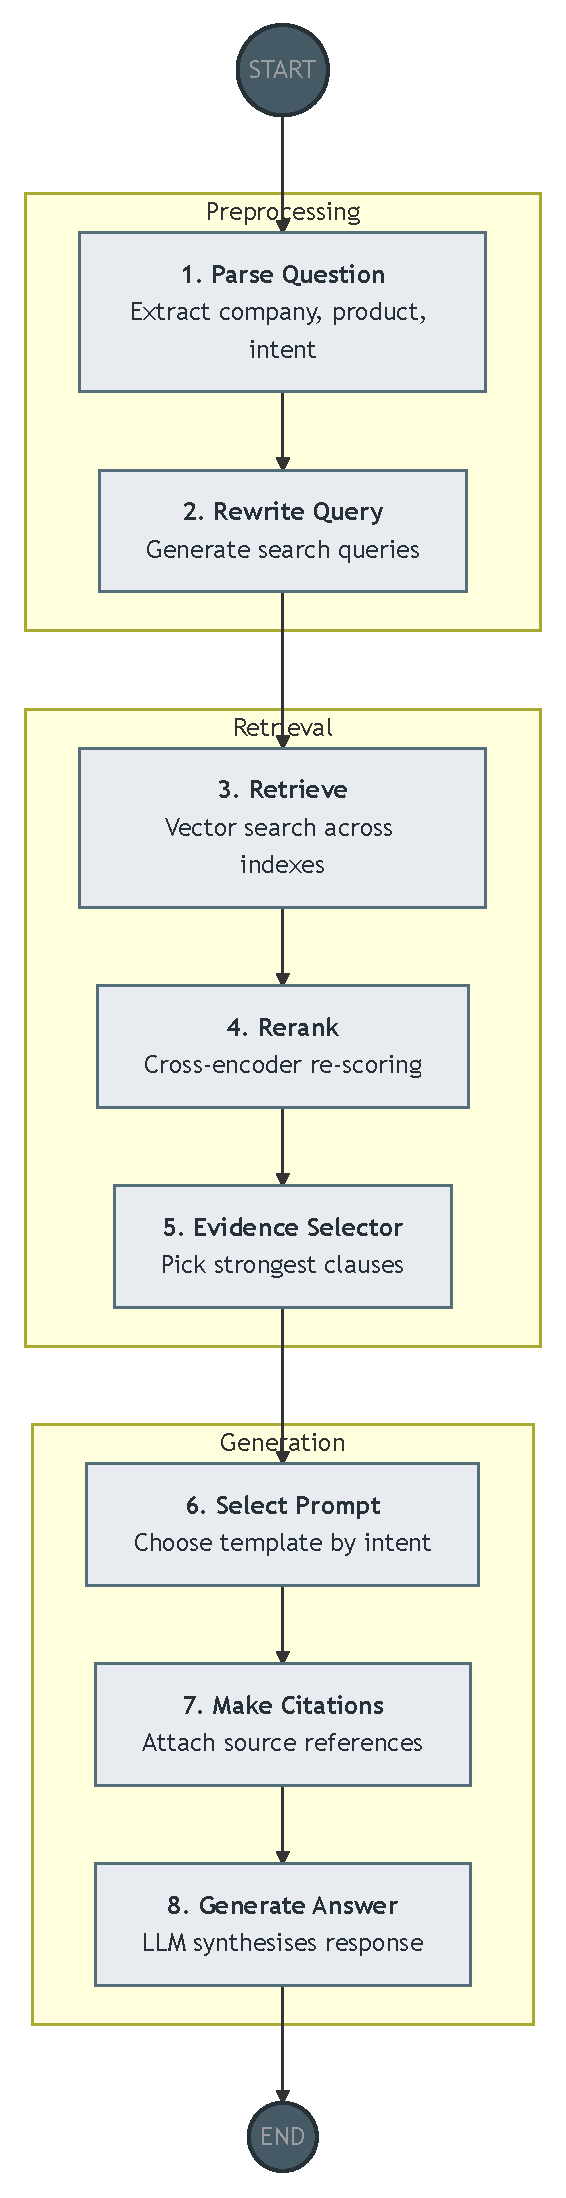
\includegraphics{../code/data/diagrams/deterministic.pdf}
  \end{adjustbox}
  \zrodlo{opracowanie własne}
\end{figure}

\begin{figure}[H]
  \caption{Architektura planer--wykonawca}\label{fig:graf-architektury-planer-wykonawca}
  \centering
  \begin{adjustbox}{max width=0.85\textwidth,
    max totalheight=0.82\textheight, keepaspectratio}
    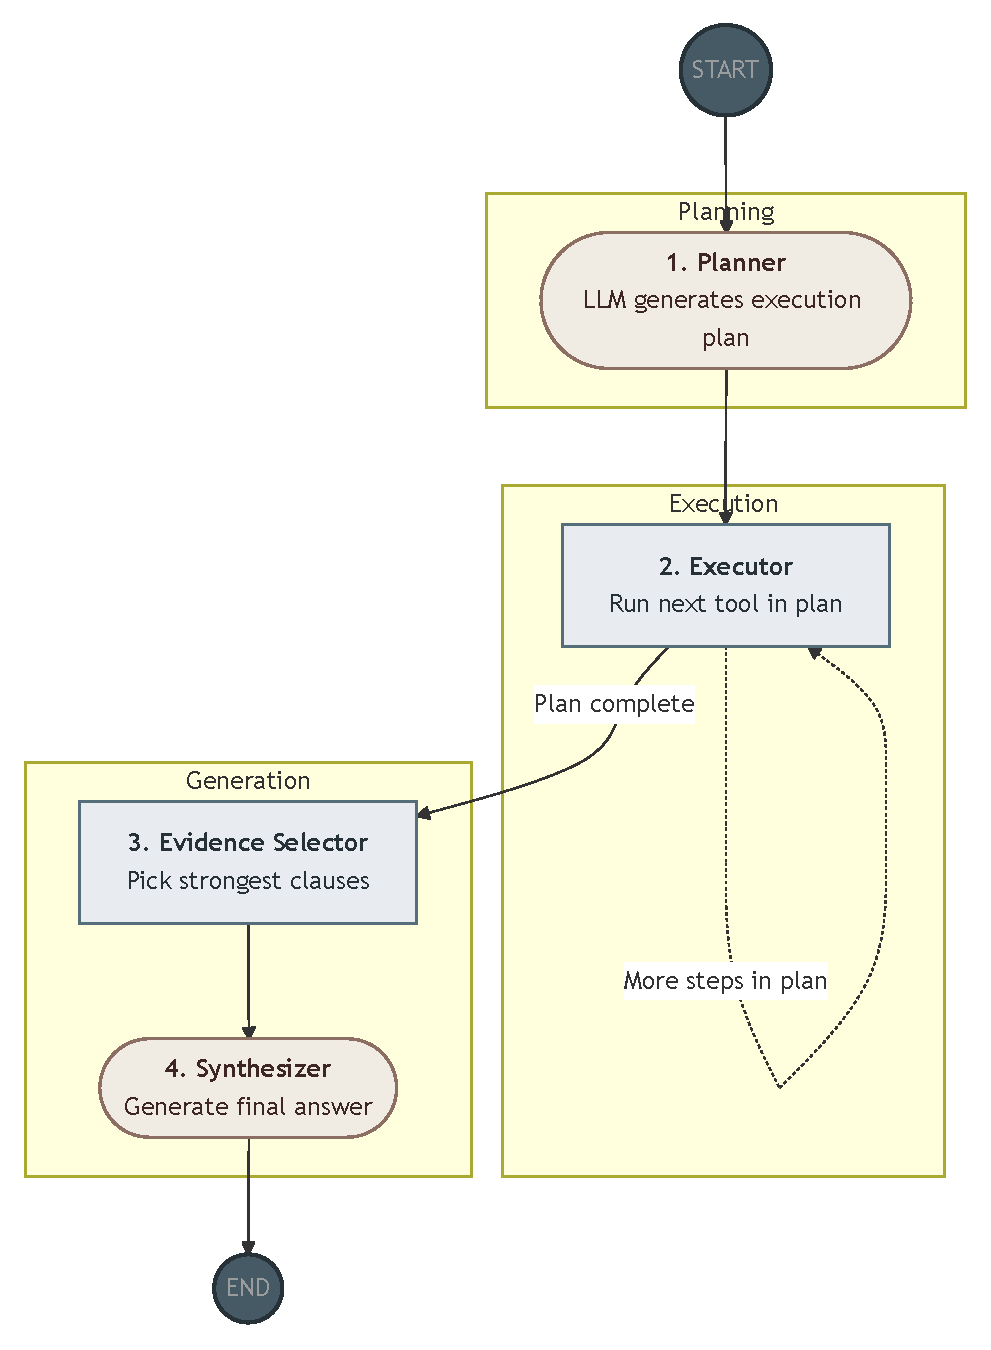
\includegraphics{../code/data/diagrams/planner_executor.pdf}
  \end{adjustbox}
  \zrodlo{opracowanie własne}
\end{figure}

\begin{figure}[H]
  \caption{Architektura router--specjalista}\label{fig:graf-architektury-router-specjalista}
  \centering
  \begin{adjustbox}{max width=0.85\textwidth,
    max totalheight=0.82\textheight, keepaspectratio}
    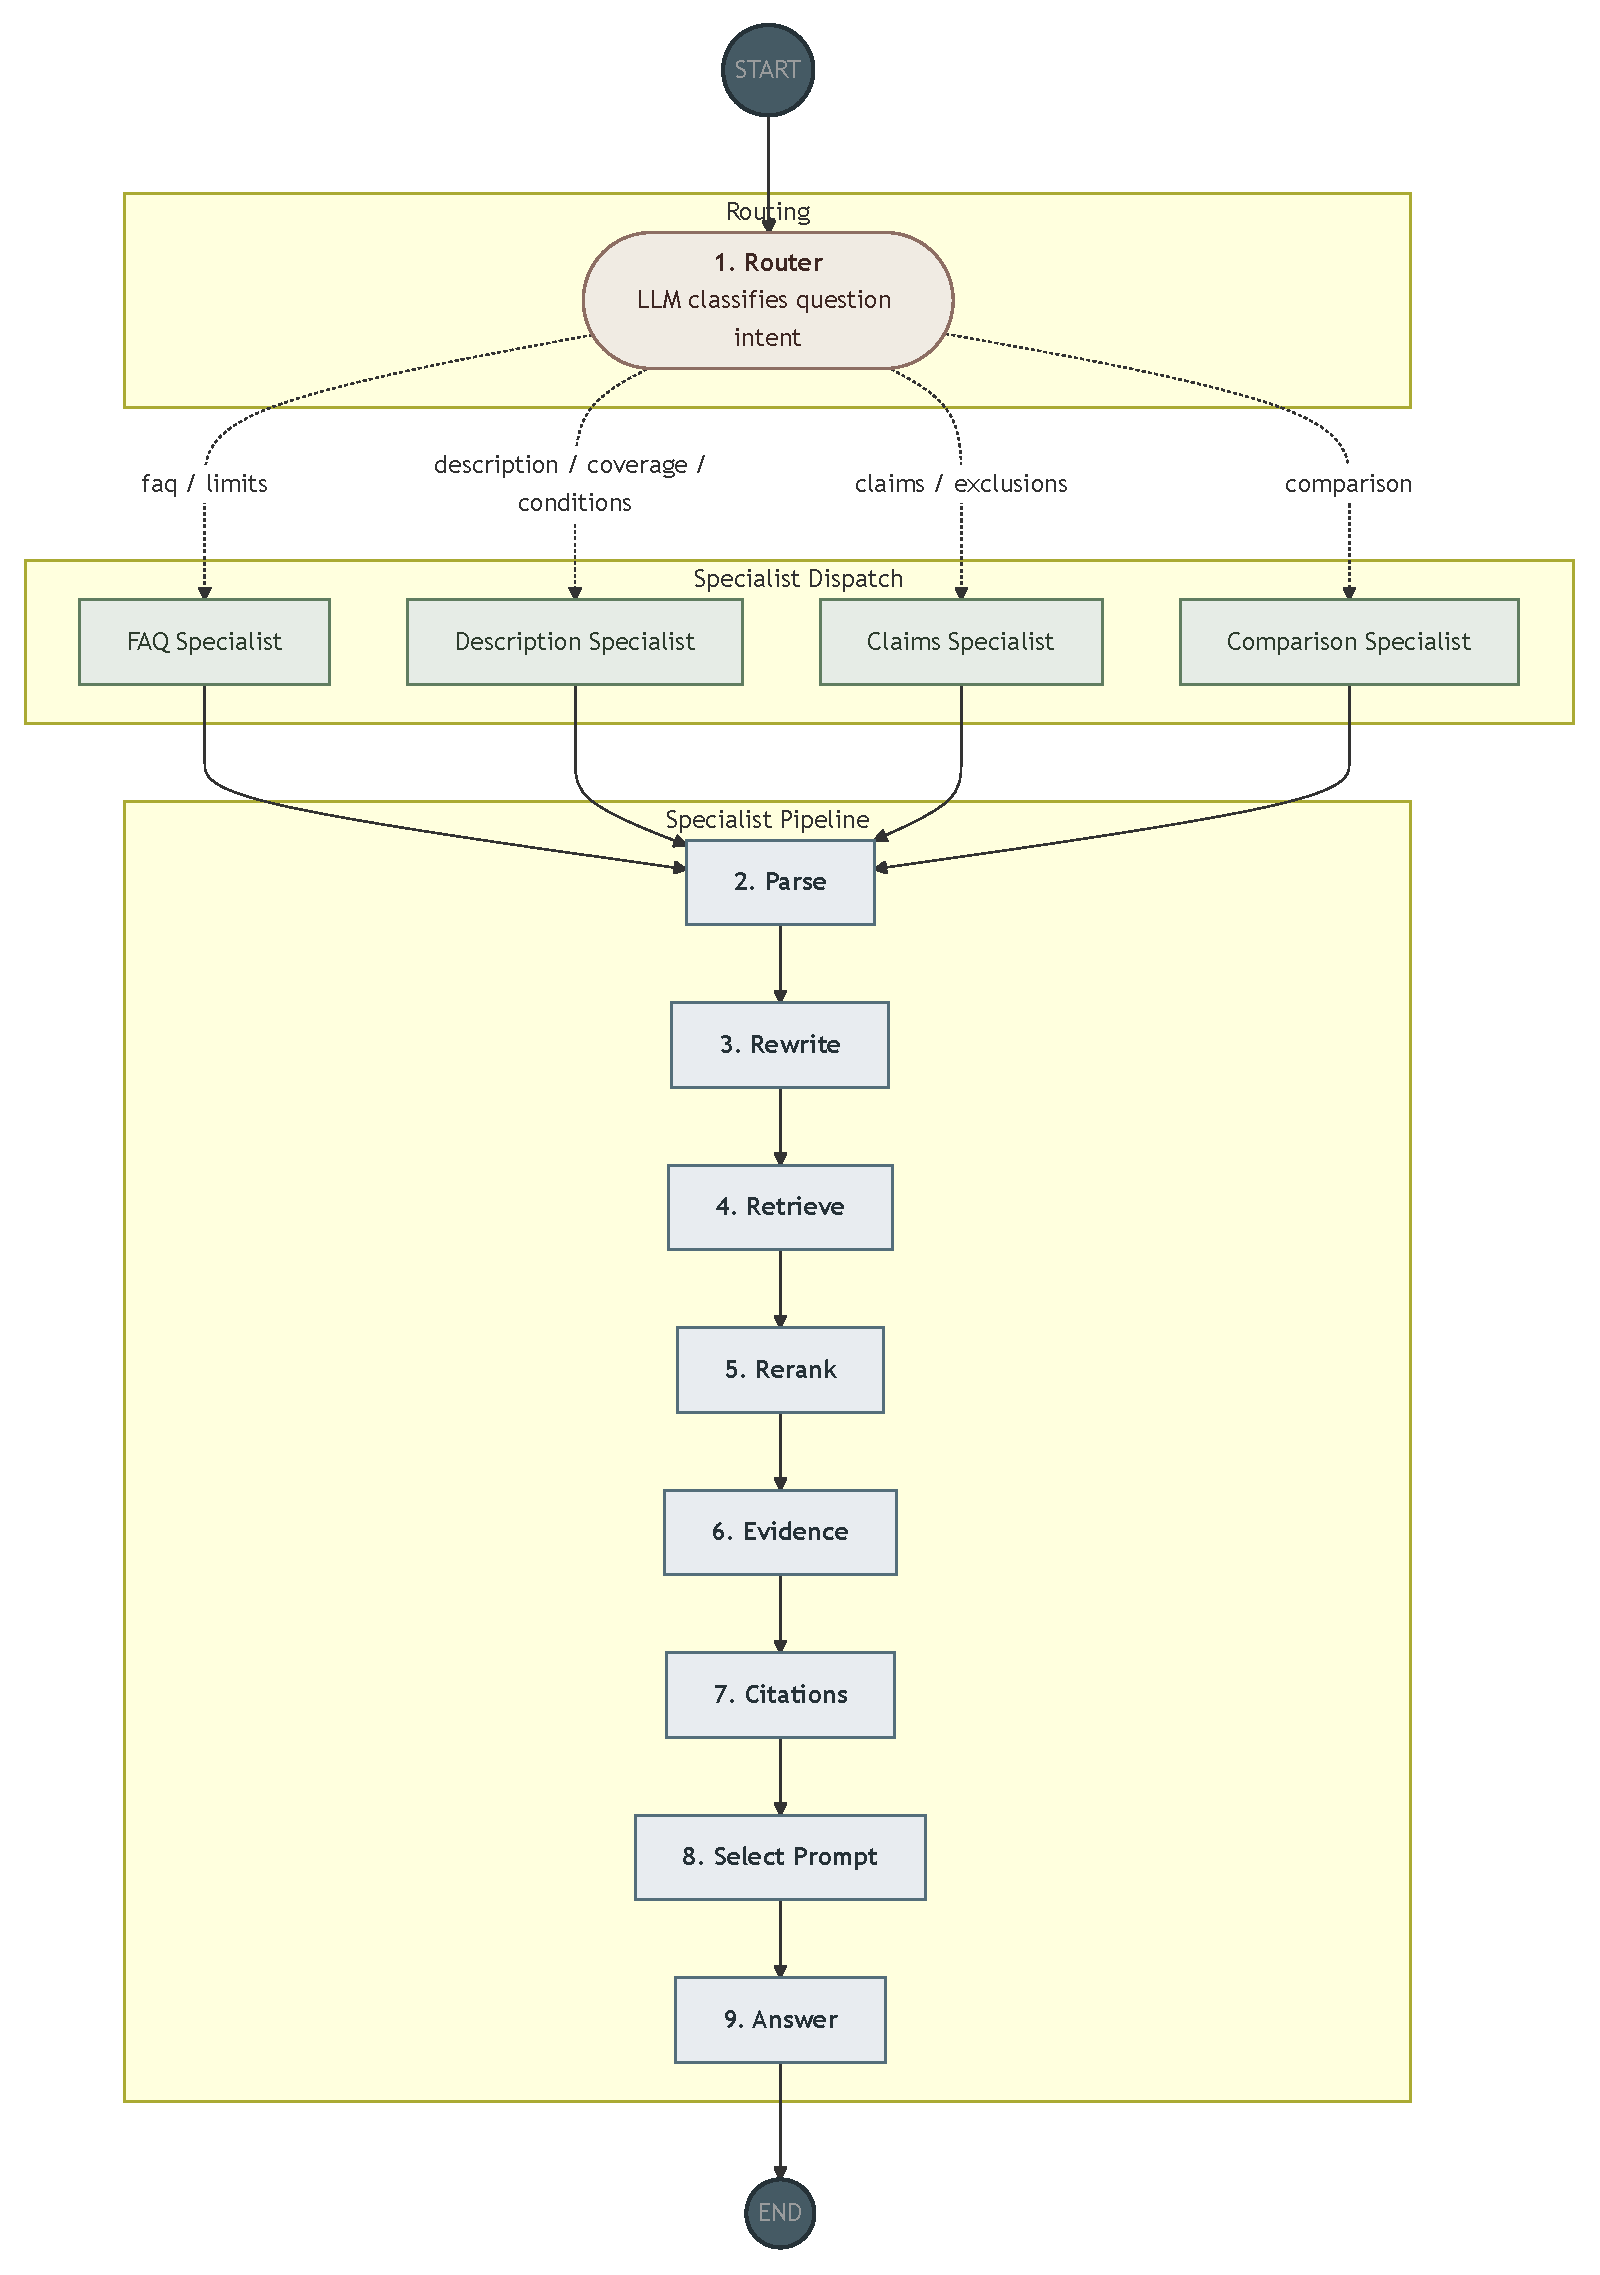
\includegraphics{../code/data/diagrams/router_specialist.pdf}
  \end{adjustbox}
  \zrodlo{opracowanie własne}
\end{figure}

\begin{figure}[H]
  \caption{Architektura tablicowa}\label{fig:graf-architektury-tablicowej}
  \centering
  \begin{adjustbox}{max width=0.85\textwidth,
    max totalheight=0.82\textheight, keepaspectratio}
    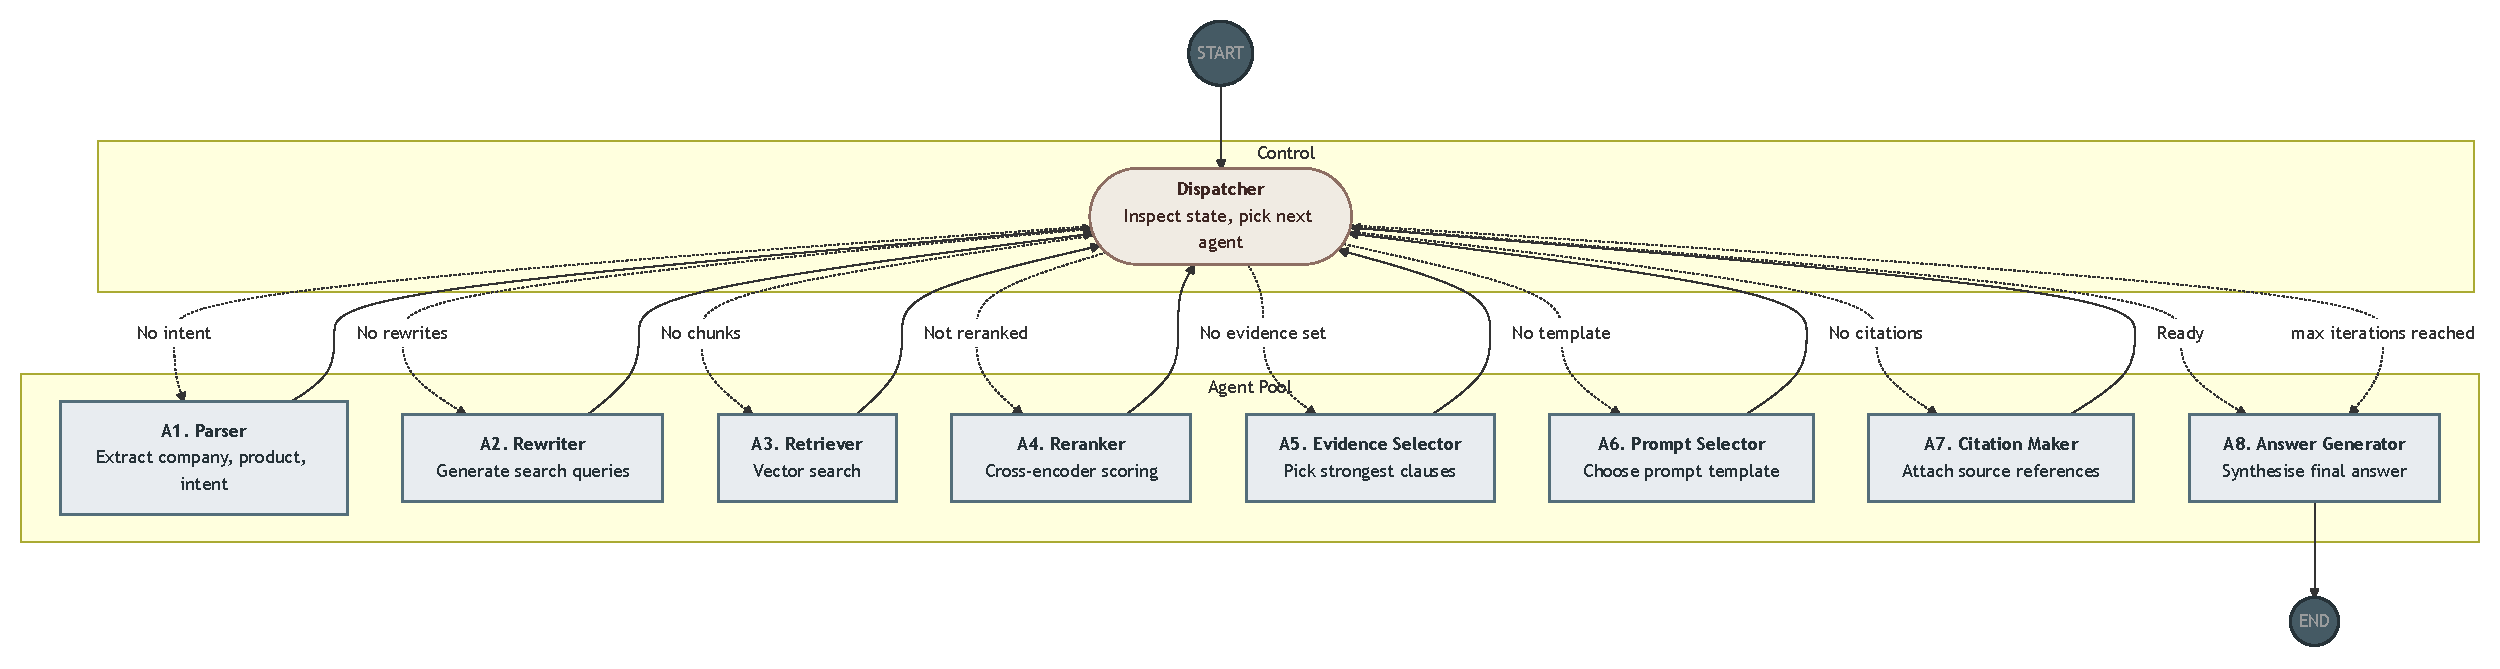
\includegraphics{../code/data/diagrams/blackboard.pdf}
  \end{adjustbox}
  \zrodlo{opracowanie własne}
\end{figure}

\begin{figure}[H]
  \caption{Architektura hierarchiczna}\label{fig:graf-architektury-hierarchicznej}
  \centering
  \begin{adjustbox}{max width=0.85\textwidth,
    max totalheight=0.82\textheight, keepaspectratio}
    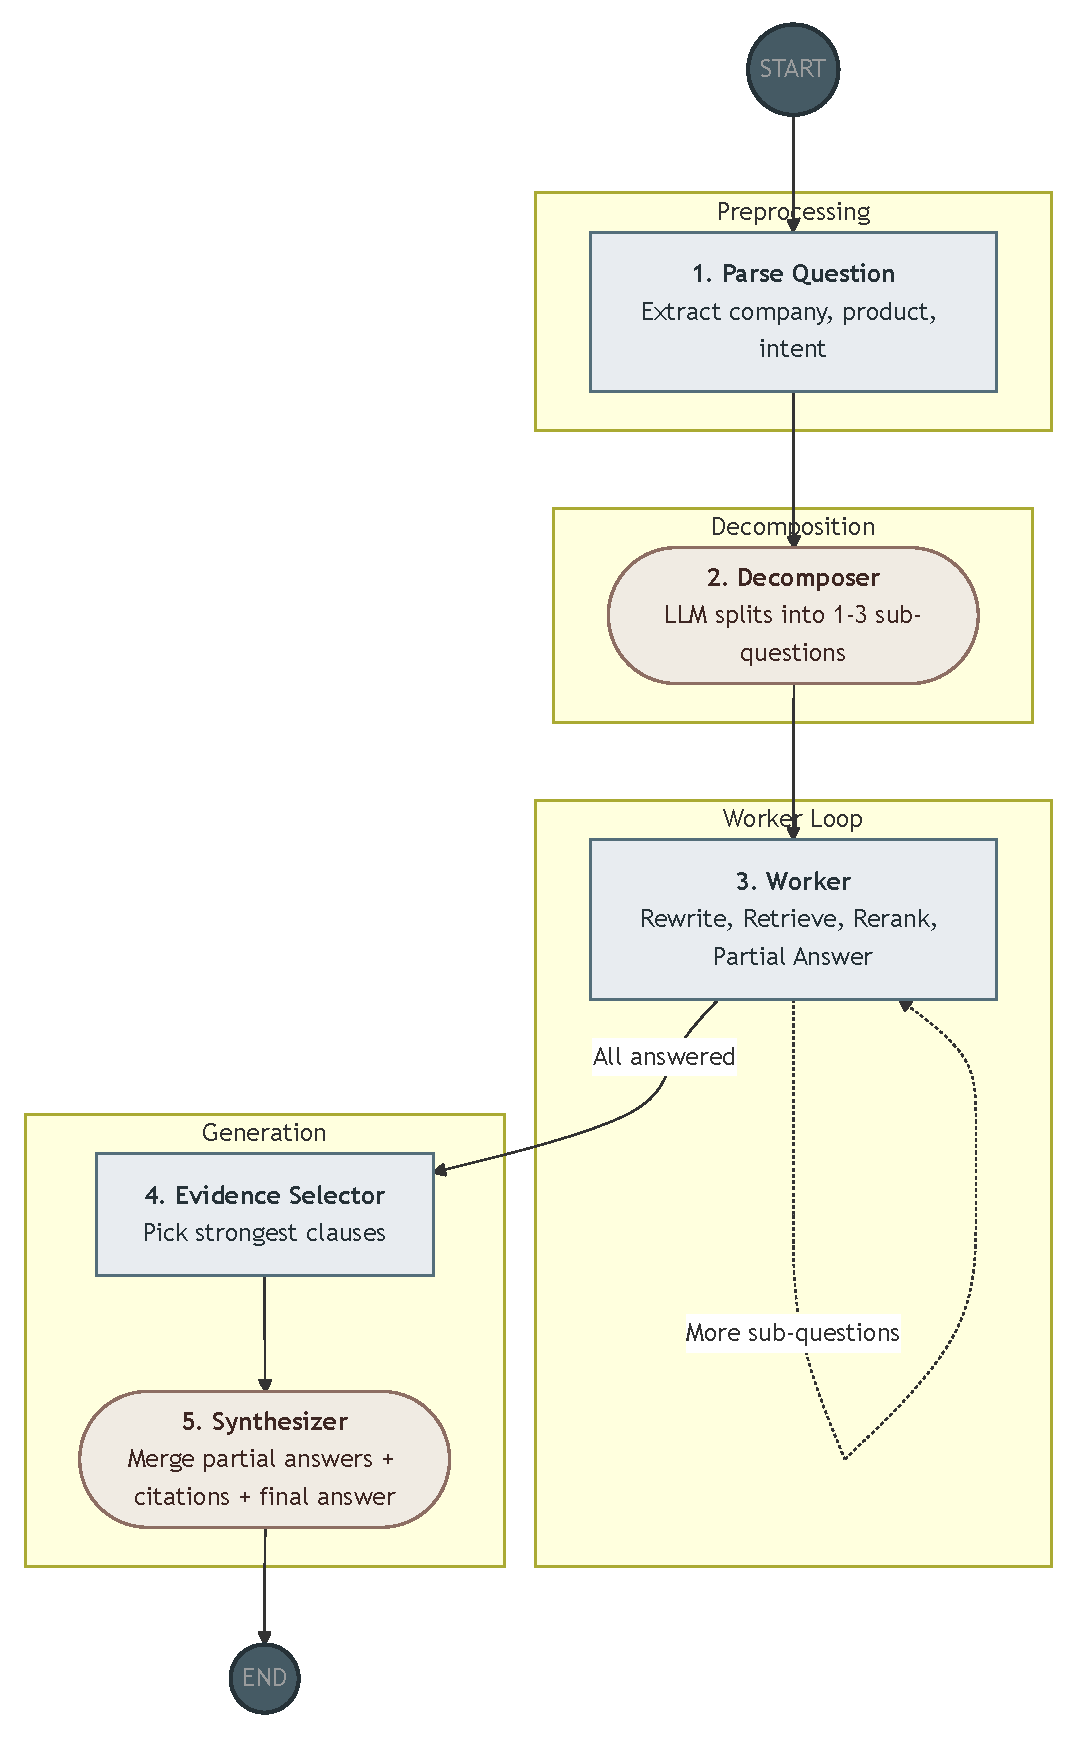
\includegraphics{../code/data/diagrams/hierarchical.pdf}
  \end{adjustbox}
  \zrodlo{opracowanie własne}
\end{figure}

\begin{figure}[H]
  \caption{Architektura ReAct}\label{fig:graf-architektury-react}
  \centering
  \begin{adjustbox}{max width=0.85\textwidth,
    max totalheight=0.82\textheight, keepaspectratio}
    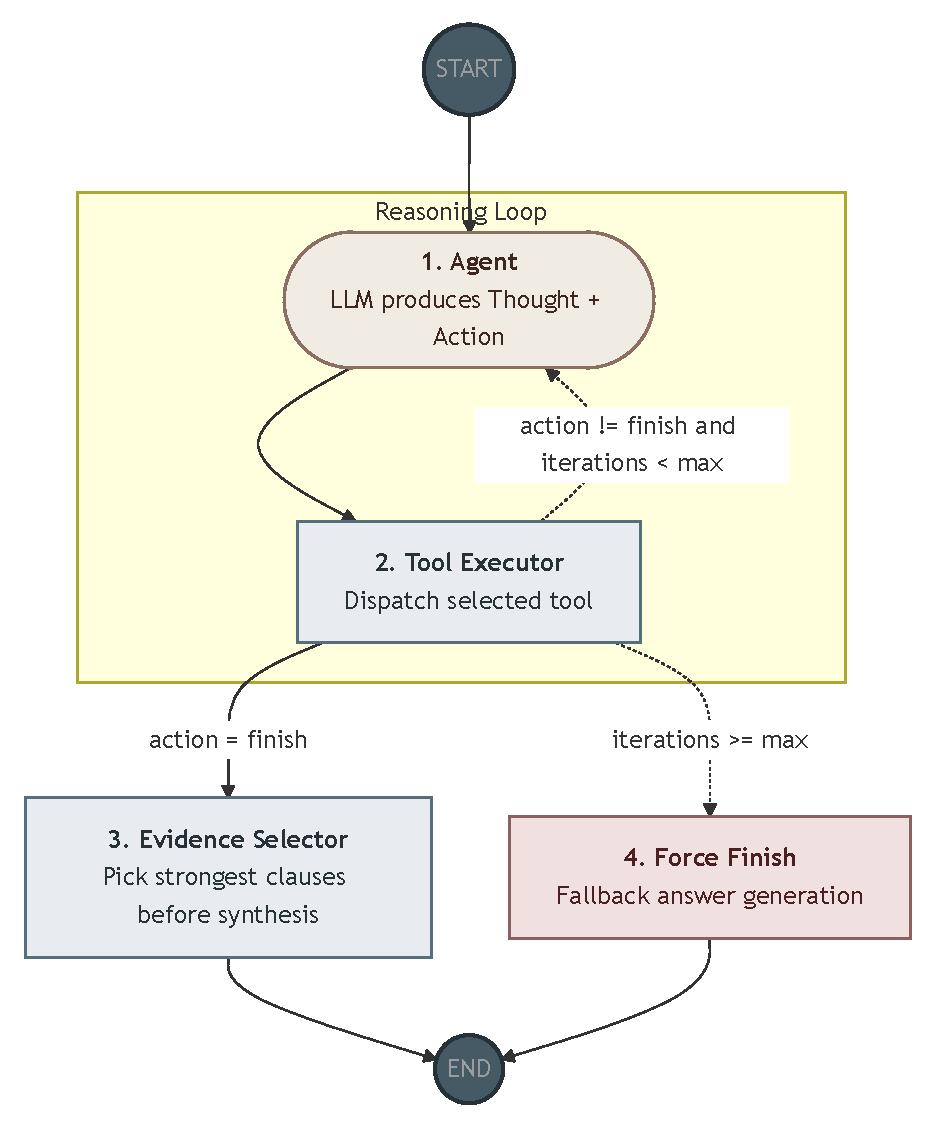
\includegraphics{../code/data/diagrams/react.pdf}
  \end{adjustbox}
  \zrodlo{opracowanie własne}
\end{figure}

\end{document}